% -*- Mode:TeX -*-

%% IMPORTANT: The official thesis specifications are available at:
%%
%%            Please verify your thesis' formatting and copyright
%%            assignment before submission.  If you notice any
%%            discrepancies between these templates and the
%%            MIT Libraries' specs, please let us know
%%            by e-mailing thesis@mit.edu

%% The documentclass options along with the pagestyle can be used to generate
%% a technical report, a draft copy, or a regular thesis.  You may need to
%% re-specify the pagestyle after you \include  cover.tex.  For more
%% information, see the first few lines of mitthesis.cls. 

%\documentclass[12pt,vi,twoside]{mitthesis}
%%
%%  If you want your thesis copyright to you instead of MIT, use the
%%  ``vi'' option, as above.
%%
%\documentclass[12pt,twoside,leftblank]{mitthesis}
%%
%% If you want blank pages before new chapters to be labelled ``This
%% Page Intentionally Left Blank'', use the ``leftblank'' option, as
%% above. 
% Add all your packages here


\documentclass[12pt,twoside]{mitthesis}
\usepackage[subpreambles=true]{standalone}
\usepackage{enumerate}
\usepackage{graphicx}
\usepackage{booktabs}
%\def\spanishoptions{mexico}
%\usepackage[spanish]{babel}
%\usepackage[T1]{fontenc}
%\usepackage[utf8]{inputenc}
\usepackage{amsmath}
\usepackage{bm}
%\usepackage{subcaption}
\usepackage{subfigure}
\usepackage{lgrind}
\usepackage{listings}
\usepackage{color}
\usepackage{float}
\usepackage{placeins}
\usepackage{times}

\usepackage{algorithm}
\usepackage{algorithmicx}
\usepackage{algpseudocode}

\usepackage{ifxetex}
\usepackage{tikz}

%For code Highlight
\usepackage[utf8]{inputenc}
\usepackage[english]{babel}
\usepackage{minted}
\usepackage{url}

\usepackage{lipsum}

%\usepackage[a4paper,margin=1cm,landscape]{geometry}
\usetikzlibrary{positioning,shapes,shadows,arrows}
 
%%%<
\usepackage{verbatim}
%\usepackage[active,tightpage]{preview}

\ifxetex
  \usepackage{fontspec}
\else
  \usepackage[T1]{fontenc}
  \usepackage[utf8]{inputenc}
  \usepackage{lmodern}
\fi

\usepackage{caption}
%\DeclareCaptionFormat{myformat}{#1#2#3}
\newlength\myindention
\DeclareCaptionFormat{myformat}%
{#1#2#3 \hspace*{\myindention}}
\captionsetup{format=myformat}
% \captionsetup[lstlisting]{position=bottom,format=myformat}
\renewcommand{\lstlistingname}{Algoritmo}

%\bibliographystyle{named}

% Include the subfolders

%\newcommand*{\Exp2}{../extras/experimentos/exp_02}
%\newcommand*{\Exp3}{../extras/experimentos/exp_03}
\usepackage{import}

\usepackage{fancyhdr}
\pagestyle{fancy}

\fancyhead{}
\fancyfoot{}

%\fancyhead[RO,RE]{\fontsize{10}{12} \selectfont \thepage}
\fancyhead[LO]{\fontsize{10}{12} \selectfont \leftmark}
\fancyhead[LE]{\fontsize{10}{12} \selectfont \leftmark}

\renewcommand{\headrulewidth}{0.0pt}
\renewcommand{\footrulewidth}{0.0pt}

%\addto\captionsspanish{%
%  \renewcommand{\appendixname}%
%    {Anexos}%
%}

\PassOptionsToPackage{hyphens}{url}\usepackage{hyperref}

\usepackage{blindtext}
\usepackage{etoolbox}
\patchcmd{\chapter}{plain}{fancy}{}{}

% For list caption

\renewcommand{\lstlistingname}{Codigo}% Listing -> Codigo
\renewcommand{\lstlistlistingname}{Índice de \lstlistingname s}

\addto\captionsenglish{
   \renewcommand\listfigurename{Índice de Figuras}}

\addto\captionsenglish{
  \renewcommand\figurename{Fig}
}

\addto\captionsenglish{
  \renewcommand\contentsname{Índice general}
}

\captionsetup[table]{name=Tabla}

\AtBeginDocument{%
  \renewcommand{\lstlistingname}{Codigo}
}

\addto\captionsenglish{%
  \renewcommand{\lstlistingname}{Codigo}
}

\addto\captionsenglish{\renewcommand{\chaptername}{Capitulo}}

\renewcommand{\chaptername}{Capítulo}

\renewcommand{\listingscaption}{Codigo}
%\addto\captionsenglish{
%  \renewcommand
%}

% List of equations
\usepackage{tocbibind}
\usepackage{tocloft}
\usepackage{xpatch}
\newcommand{\listequationsname}{List of Equations}
\newlistof{myequations}{equ}{\listequationsname}
\newcommand{\myequations}[1]{%
\addcontentsline{equ}{myequations}{\protect\numberline{\theequation}#1}\par}
\xpretocmd{\listofmyequations}{\addcontentsline{toc}{chapter}{\listequationsname}}{}{}

\def\all{all}
% \ifx\files\all \typeout{Including all files.} \else \typeout{Including only \files.} \includeonly{\files} \fi

\usepackage[most]{tcolorbox}
\newtcblisting{Heardlisting}[2][]{%
empty,
boxsep=0pt,left=0pt,right=0pt,boxrule=2pt,leftrule=0pt,rightrule=0pt,
lefthand width=.4\linewidth,
segmentation engine=path,
segmentation style={solid,line width=1pt},
comment side listing,
fontupper=\itshape\sffamily,
listing options={% put any listing options here
    language={Haskell},
    aboveskip=0pt, belowskip=0pt,
    basicstyle=\ttfamily,columns=fullflexible},
comment={#2},#1
} 
 
\begin{document}
%\subimport{extras/experimentos/exp_01/}{test.tex}
% -*-latex-*-
% 
% For questions, comments, concerns or complaints:
% thesis@mit.edu
% 
%
% $Log: cover.tex,v $
% Revision 1.8  2008/05/13 15:02:15  jdreed
% Degree month is June, not May.  Added note about prevdegrees.
% Arthur Smith's title updated
%
% Revision 1.7  2001/02/08 18:53:16  boojum
% changed some \newpages to \cleardoublepages
%
% Revision 1.6  1999/10/21 14:49:31  boojum
% changed comment referring to documentstyle
%
% Revision 1.5  1999/10/21 14:39:04  boojum
% *** empty log message ***
%
% Revision 1.4  1997/04/18  17:54:10  othomas
% added page numbers on abstract and cover, and made 1 abstract
% page the default rather than 2.  (anne hunter tells me this
% is the new institute standard.)
%
% Revision 1.4  1997/04/18  17:54:10  othomas
% added page numbers on abstract and cover, and made 1 abstract
% page the default rather than 2.  (anne hunter tells me this
% is the new institute standard.)
%
% Revision 1.3  93/05/17  17:06:29  starflt
% Added acknowledgements section (suggested by tompalka)
% 
% Revision 1.2  92/04/22  13:13:13  epeisach
% Fixes for 1991 course 6 requirements
% Phrase "and to grant others the right to do so" has been added to 
% permission clause
% Second copy of abstract is not counted as separate pages so numbering works
% out
% 
% Revision 1.1  92/04/22  13:08:20  epeisach

% NOTE:
% These templates make an effort to conform to the MIT Thesis specifications,
% however the specifications can change.  We recommend that you verify the
% layout of your title page with your thesis advisor and/or the MIT 
% Libraries before printing your final copy.

%% \title{Clasificaci??n de Estados Afectivos usando Din??mica de Tecleo yde Rat??n en Programaci??n de Software}

%% \author{Amaury Hern??ndez ??guila}
%% % If you wish to list your previous degrees on the cover page, use the 
%% % previous degrees command:
%% %       \prevdegrees{A.A., Harvard University (1985)}
%% % You can use the \\ command to list multiple previous degrees
%% %       \prevdegrees{B.S., University of California (1978) \\
%% %                    S.M., Massachusetts Institute of Technology (1981)}
%% \department{Divisi??n de Estudios de Posgrado e Investigaci??n}

%% % If the thesis is for two degrees simultaneously, list them both
%% % separated by \and like this:
%% % \degree{Doctor of Philosophy \and Master of Science}
%% \degree{Maestro en Ciencias Computacionales}

%% % As of the 2007-08 academic year, valid degree months are September, 
%% % February, or June.  The default is June.
%% \degreemonth{Julio}
%% \degreeyear{2014}
%% \thesisdate{8 de septiembre, 2014}
%% \copyrightnoticetext{Tijuana, Baja California, M??xico}

%% %% By default, the thesis will be copyrighted to MIT.  If you need to copyright
%% %% the thesis to yourself, just specify the `vi' documentclass option.  If for
%% %% some reason you want to exactly specify the copyright notice text, you can
%% %% use the \copyrightnoticetext command.  
%% %\copyrightnoticetext{\copyright IBM, 1990.  Do not open till Xmas.}

%% % If there is more than one supervisor, use the \supervisor command
%% % once for each.
%% %\supervisor{Dr. Jos?? Mario Garc??a Valdez}{.}

%% % This is the department committee chairman, not the thesis committee
%% % chairman.  You should replace this with your Department's Committee
%% % Chairman.
%% \chairman{M.C. Alejandra Mancilla Soto}{.}

% Make the titlepage based on the above information.  If you need
% something special and can't use the standard form, you can specify
% the exact text of the titlepage yourself.  Put it in a titlepage
% environment and leave blank lines where you want vertical space.
% The spaces will be adjusted to fill the entire page.  The dotted
% lines for the signatures are made with the \signature command.
%\maketitle

\begin{titlepage}
  \begin{center}
  \textsc{\Large SEP}
  \:\:\:\:\:\:\:\:\:\:\:\:\:\:\:\:\:\:\:\:\:\:\:\:\:\:\:\:\:\:\:\:\:\:\:\:
\:\:\:\:\:\:\:\:\:\:\:\:\:\:\:\:\:\:\:\:\:\:\:\:\:\:\:\:\:\:\:\:\:\:\:\:
\:\:\:\:\:\:\:\:\:\:\:\:\:\:\:\:
  \textsc{\Large TNM}~\\[1cm]
  \textsc{\Large INSTITUTO TECNÓLOGICO DE TIJUANA}~\\[1cm]
  \textsc{\Large División de Estudios de Posgrado e
    Investigación}~\\[0.5cm]

    
\includegraphics[width=0.25\textwidth]{./logos.png}~\\[1cm]

    %% \textsc{\LARGE Trading Strategy for Foreign Exchange Markets based on Computational Intelligence, Multi-Agent Systems and Logarithmic Spirals}~\\[1.5cm]
    
    \textsc{\LARGE Generación procedural de niveles para el videojuego de angry birds utilizando computo evolutivo}~\\[1.5cm]

%% \textsc{por}~\\[0.5cm]
%% \textsc{\Large Amaury Hernández Águila}~\\[1.0cm]

%% \textsc{Tesis para obtener el grado de}~\\[0.5cm]
%% \textsc{\Large Doctor en Ciencias Computacionales}~\\[0.5cm]
%% \textsc{}~\\[0.5cm]

%% \textsc{Febrero 2019}~\\[0.2cm]
%% \textsc{Tijuana, Baja California, México}~\\[1cm]

\begin{minipage}{1\textwidth}
  \begin{flushright} \large
    TRABAJO DE TESIS~\\[0.5cm]
    \small
    PRESENTADO POR~\\[0.5cm]
    \large
    JAIME SALINAS HERNÁNDEZ ~\\[0.5cm]
    \small
    PARA OBTENER EL GRADO DE~\\[0.5cm]
    \large
    MAESTRO EN CIENCIAS~\\
    EN COMPUTACIÓN~\\[0.5cm]
    \small
    DIRECTOR DE TESIS~\\
    \large
    DR. JOSÉ MARIO GARCÍA VALDEZ~\\[0.5cm]
    \small
    Tijuana, B.C., México. Noviembre 2019
  \end{flushright}
\end{minipage}

%% \begin{minipage}{1.5\textwidth}
%%   \begin{flushleft} \large
%%     \emph{Director:}\\
%%     Dr. Jos?? Mario \textsc{Garc??a Valdez}
%%   \end{flushleft}
%% \end{minipage}

%% \begin{minipage}{1.5\textwidth}
%% \begin{flushleft} \large
%% \emph{Co-Directora:} \\
%% M.C. Alejandra \textsc{Mancilla Soto}
%% \end{flushleft}
%% \end{minipage}

\vfill

  \end{center}

\end{titlepage}

% The abstractpage environment sets up everything on the page except
% the text itself.  The title and other header material are put at the
% top of the page, and the supervisors are listed at the bottom.  A
% new page is begun both before and after.  Of course, an abstract may
% be more than one page itself.  If you need more control over the
% format of the page, you can use the abstract environment, which puts
% the word "Abstract" at the beginning and single spaces its text.

%% You can either \input (*not* \include) your abstract file, or you can put
%% the text of the abstract directly between the \begin{abstractpage} and
%% \end{abstractpage} commands.

% First copy: start a new page, and save the page number.
%\cleardoublepage
% Uncomment the next line if you do NOT want a page number on your
% abstract and acknowledgments pages.
\pagestyle{empty}
\setcounter{savepage}{\thepage}
\begin{abstractpage}
% $Log: abstract.tex,v $
% Revision 1.1  93/05/14  14:56:25  starflt
% Initial revision
% 
% Revision 1.1  90/05/04  10:41:01  lwvanels
% Initial revision
% 
%
%% The text of your abstract and nothing else (other than comments) goes here.
%% It will be single-spaced and the rest of the text that is supposed to go on
%% the abstract page will be generated by the abstractpage environment.  This
%% file should be \input (not \include 'd) from cover.tex 

En el documento de tesis presentado se propone un algoritmo evolutivo que
utiliza enfoques de la teoría de open-ended evolution para generar niveles para
el videojuego de Angry Birds. Los niveles utilizados en este juego se componen
de elementos tales como una cierta cantidad de aves que el usuario puede
disparar a manera de resortera, una cantidad determinada de puerquitos que se
requieren eliminar como objetivo para avanzar en los niveles, así como de una
determinada cantidad de piezas que conforman estructuras que sirven como
obstáculos para el usuario. El objetivo del sistema que aquí se propone es el de
generar las diferentes estructuras que se presentan en el juego, teniendo en
cuenta las características que deben de cumplir para poder ser utilizadas, es
decir que sean llamativas y funcionales. Para esto se propone una búsqueda de
múltiples capas, la primera parte se trata de construir estructuras utilizando
piezas básicas del juego, posteriormente utilizar estas estructuras como base y
continuar generando desde ese punto para obtener estructuras más complejas. Se
utilizará un enfoque basado en open-ended evolution el cual será utilizado para
la evolución de las estructuras con el objetivo de crear otras más complejas y
diversas entre sí. La función de aptitud que se utilizara para evaluar los
niveles considera la complejidad de los niveles y que tan diferentes son estos
del resto de la población de niveles generada. Los experimentos realizados
muestran que un enfoque evolutivo permite la generación de niveles que logran
ser novedosos y son interesantes para ser jugados.
 
\clearpage
\section*{Abstract}

In this thesis, we propose an evolutionary algorithm that follows an open-ended
evolution approach to generate levels for the Angry Birds video game. The levels
themselves are composed of a set of birds that the player can throw with a
slingshot, a certain amount of pigs that they must destroy, and a given number
of pieces that conform structures that may or may not protect the pigs from
birds thrown at them. The current goal is the generation of diverse structures
that are playable in the game, having the additional characteristics of being
fun and enjoyable. We propose a multi-layered search, first constructing
composite structures from basic blocks, to then build more complex structures
building from these composites. We follow an open-ended evolution approach in
which the evolution of structures is not guided towards a single objective but
is rather free to evolve and generate novelty or diversity. The fitness function
we use to evaluate the proposed levels considers how complex levels have become
and how different they are from the rest of the population. The experiments
conducted show that an evolutionary approach allows the generation of levels
that are novel and interesting to play.
\end{abstractpage}

% Additional copy: start a new page, and reset the page number.  This way,
% the second copy of the abstract is not counted as separate pages.
% Uncomment the next 6 lines if you need two copies of the abstract
% page.
% \setcounter{page}{\thesavepage}
% \begin{abstractpage}
% % $Log: abstract.tex,v $
% Revision 1.1  93/05/14  14:56:25  starflt
% Initial revision
% 
% Revision 1.1  90/05/04  10:41:01  lwvanels
% Initial revision
% 
%
%% The text of your abstract and nothing else (other than comments) goes here.
%% It will be single-spaced and the rest of the text that is supposed to go on
%% the abstract page will be generated by the abstractpage environment.  This
%% file should be \input (not \include 'd) from cover.tex 

En el documento de tesis presentado se propone un algoritmo evolutivo que
utiliza enfoques de la teoría de open-ended evolution para generar niveles para
el videojuego de Angry Birds. Los niveles utilizados en este juego se componen
de elementos tales como una cierta cantidad de aves que el usuario puede
disparar a manera de resortera, una cantidad determinada de puerquitos que se
requieren eliminar como objetivo para avanzar en los niveles, así como de una
determinada cantidad de piezas que conforman estructuras que sirven como
obstáculos para el usuario. El objetivo del sistema que aquí se propone es el de
generar las diferentes estructuras que se presentan en el juego, teniendo en
cuenta las características que deben de cumplir para poder ser utilizadas, es
decir que sean llamativas y funcionales. Para esto se propone una búsqueda de
múltiples capas, la primera parte se trata de construir estructuras utilizando
piezas básicas del juego, posteriormente utilizar estas estructuras como base y
continuar generando desde ese punto para obtener estructuras más complejas. Se
utilizará un enfoque basado en open-ended evolution el cual será utilizado para
la evolución de las estructuras con el objetivo de crear otras más complejas y
diversas entre sí. La función de aptitud que se utilizara para evaluar los
niveles considera la complejidad de los niveles y que tan diferentes son estos
del resto de la población de niveles generada. Los experimentos realizados
muestran que un enfoque evolutivo permite la generación de niveles que logran
ser novedosos y son interesantes para ser jugados.
 
\clearpage
\section*{Abstract}

In this thesis, we propose an evolutionary algorithm that follows an open-ended
evolution approach to generate levels for the Angry Birds video game. The levels
themselves are composed of a set of birds that the player can throw with a
slingshot, a certain amount of pigs that they must destroy, and a given number
of pieces that conform structures that may or may not protect the pigs from
birds thrown at them. The current goal is the generation of diverse structures
that are playable in the game, having the additional characteristics of being
fun and enjoyable. We propose a multi-layered search, first constructing
composite structures from basic blocks, to then build more complex structures
building from these composites. We follow an open-ended evolution approach in
which the evolution of structures is not guided towards a single objective but
is rather free to evolve and generate novelty or diversity. The fitness function
we use to evaluate the proposed levels considers how complex levels have become
and how different they are from the rest of the population. The experiments
conducted show that an evolutionary approach allows the generation of levels
that are novel and interesting to play.
% \end{abstractpage}

%\cleardoublepage
\clearpage

\section*{Agradecimientos}

Agradezco principalmente a mi familia, quien sin duda alguna me brindó todo el
apoyo y comprensión necesaria para poder continuar con mi desarrollo académico,
su motivación brindada para ayudarme a salir adelante es sin duda lo que me
ayudó a llegar tan lejos.

Agradezco a mis amigos y compañeros de maestría Sergio y Eduardo con quienes me
embarqué en esta aventura de conocimiento, agradezco su compañía, su tiempo y su
apoyo.

Agradezco a los profesores con quienes cursé mis materias, M.C.C. Alejandra
Mancilla, Dr. Fevrier Valdez, Dra Denisse Paulette, Dra. Gabriela Martínez,
Dra. Claudia Gonzalez, Dr. Jose Soria, Dr Oscar Castillo, Dra. Patricia Melin,
gracias al conocimiento adquirido por ustedes es que logré llegar hasta aqui.

Un gran agradecimiento a mi director de tesis el Dr. Mario Garcia Valdez por el
apoyo que me brindó, su paciencia con mis errores, el tiempo que dedicó a
ayudarme con mis dudas y la comprensión brindada.

Finalmente, le agradezco al Institiuto Tecnológico de Tijuana por la educación de
alta calidad recibida, de igual manera agradezco a CONACYT por el apoyo otorgado
a travéz del Programa Nacional de Posgrados de Calidad (número de CVU 797248).


%%%%%%%%%%%%%%%%%%%%%%%%%%%%%%%%%%%%%%%%%%%%%%%%%%%%%%%%%%%%%%%%%%%%%%
% -*-latex-*-

% Some departments (e.g. 5) require an additional signature page.  See
% signature.tex for more information and uncomment the following line if
% applicable.
% % -*- Mode:TeX -*-
%
% Some departments (e.g. Chemistry) require an additional cover page
% with signatures of the thesis committee.  Please check with your
% thesis advisor or other appropriate person to determine if such a 
% page is required for your thesis.  
%
% If you choose not to use the "titlepage" environment, a \newpage
% commands, and several \vspace{\fill} commands may be necessary to
% achieve the required spacing.  The \signature command is defined in
% the "mitthesis" class
%
% The following sample appears courtesy of Ben Kaduk <kaduk@mit.edu> and
% was used in his June 2012 doctoral thesis in Chemistry. 

\begin{titlepage}
\begin{large}
This doctoral thesis has been examined by a Committee of the Department
of Chemistry as follows:

\signature{Professor Jianshu Cao}{Chairman, Thesis Committee \\
   Professor of Chemistry}

\signature{Professor Troy Van Voorhis}{Thesis Supervisor \\
   Associate Professor of Chemistry}

\signature{Professor Robert W. Field}{Member, Thesis Committee \\
   Haslam and Dewey Professor of Chemistry}
\end{large}
\end{titlepage}



%\pagestyle{plain}
\pagestyle{fancy}
\rfoot{\thepage}
%\fancyfoot[R]{\thepage}
\setcounter{page}{1}
\renewcommand{\thepage}{\roman{page}}% Roman numerals for page counter
% -*- Mode:TeX -*-
%% This file simply contains the commands that actually generate the table of
%% contents and lists of figures and tables.  You can omit any or all of
%% these files by simply taking out the appropriate command.  For more
%% information on these files, see appendix C.3.3 of the LaTeX manual. 
\tableofcontents
\newpage
\listoffigures
\newpage
\listoftables
%\newpage
%\listofmyequations
\setcounter{page}{1}
\renewcommand{\thepage}{\arabic{page}}
\chapter{Introduction}
\label{chapter:introduction}

El método de generación de contenido procedural ha sido tomado con
gran interés en el ámbito de desarrollo de videojuegos debido a los beneficios
que brinda a las compañías para poder generar contenido que pueda ser utilizado
en juegos. No es posible asociar la generación procedural de contenido con algún
aspecto especifico de la creación de videojuegos o inclusive únicamente en el
enfoque de videojuegos debido a que el tema puede ser utilizado para 
aspectos diferentes, desde la generación de áreas como en el videojuego Spelunky
\cite{RovioEntertainmentCorporation2009} \cite{Mossmouth2013}
\cite{Mossmouth2013}, la generación de historias, que sean inmersivas como en
Façade \cite{Mateas}, la generación de piezas sonoras como las que se pueden 
escuchar en Audioverdrive \cite{Holtar}, generación de efectos gráficos como
el diseño de pétalos en Petalz \cite{Risi2012}, así como otros en los enfoques
de gameplay y videojuegos completos.

Estas ideas han sido de mutuo interés entre la industria y la comunidad
científica por lo que en 2005 se originó un simposio de la IEEE en el ámbito de
Computación Inteligente y Videojuegos (Computational Intelligence and Games) el
cual posteriormente pasaría a ser una conferencia en el año 2009.

Esta conferencia tiene el fin de unir a ambos grupos de interés en un mismo
lugar con el fin de conocer sobre los avances de la computación inteligente
enfocada en juegos, dentro del marco de la misma conferencia se celebran
competencias de diferentes juegos tales como inteligencia artificial en el juego
de Hearthstone, jugar niveles de Ms. Pac-Man, competencias de agentes para ganar
en juegos de pelea y varios otros.

Dentro de estas mismas competencias se celebra la de generación de niveles para
el videojuego de Angry Birds la cual consiste primordialmente en generar niveles
que sean interesantes visualmente y sean complejos en el sentido de que sean
difíciles de completar por una persona pero que al mismo tiempo no sean
imposibles de completar, este juego fue desarrollado por la compañía Rovio
Entertainment Corporation\cite{RovioEntertainmentCorporation2009} en el año
2009, el objetivo dentro del juego consta de utilizar un número dado de aves con
diferentes efectos para eliminar puercos color verde que se encuentran
protegidos e incluso sobre estructuras de diferentes materiales y formas, en
algunos casos al golpear partes de las estructuras se crea un efecto dominó que
termina por destruir la mayoría de las misma, el juego cuenta con un
sistema de gravedad que permite que las trayectorias de tiro generen diferentes
efectos en las estructuras. En este trabajo el interés principal es que mediante el
uso del sistema de gravedad del juego se puedan crear estructuras
interesantes visualmente y que sean lo suficientemente robustas para soportar
golpes de las mismas aves y logre mantenerse en pie el mayor tiempo posible.

El objetivo principal de este proyecto es el de generar un sistema basado en
computo evolutivo que logre generar las estructuras que conformarán los niveles
del juego de Angry Birds y evaluar estas mismas estructuras mediante los
aspectos propuestos en la competencia para que sean entretenidos, complejos y con 
cierto grado de dificultad.  Los objetivos que se enmarcaran en el proyecto son los siguientes: 

\begin{itemize}
  \item Adaptar un algoritmo genético para que sea capaz de generar secuencias
  de estructuras para generar un nivel cumpliendo los requerimientos.
  \item Modificar y adaptar el software de simulación para poder obtener datos
  específicos de un nivel requeridos para su evaluación.
  \item Adaptar el método de evolución para permitir que se puedan generar
  estructuras complejas.
  \item Explorar las posibilidades de integrar alguna otra técnica de computo
  evolutivo para optimizar la generación de niveles.
\end{itemize} 

El trabajo propuesto tiene como objetivo la generación
de contenido con el cual un jugador podrá interactuar en el videojuego de
Angry Birds, cabe remarcar que el uso de métodos de generación procedural han
sido utilizados con el proposito de realizar competencias en el marco de la
conferencia del Instituto de Ingeniería Eléctrica y Electrónica (IEEE) que lleva
por nombre Conferencia de Juegos (CoG), en dicha competencia se utilizan
algoritmos capaces de generar los niveles que una persona o agente puede jugar.
En nuestro caso la metodología propuesta en este proyecto pretende servir de
base para mostrar que es posible la utilizacion de algoritmos evolutivos libres
de tal manera que el contenido generado será único y entretenido para los
usuarios. En este mismo capítulo se presentan las motivaciones para la
realización del proyecto así como la manera en que la computación evolutiva
sirve de apoyo en la industria del entretenimiento (ver la Sección
\ref{section:justification}).

El método propuesto en este documento consta de tres campos diferentes, estos
campos son Generación de Contenido Procedural y dos áreas de la computación
evolutiva las cuales son algoritmos genéticos y la evolución abierta. El
Capítulo \ref{chapter:preliminaries} está dedicado a explicar los conceptos
de estas áreas, mismos que son necesarios para comprender mejor el contenido de
los capítulos subsecuentes.

Una vez que los conceptos mostrados en el capítulo anterior han sido
vistos en el Capítulo \ref{chapter:related-work} se presentan un
conjuntos de trabajos relacionados con lo que se quiere lograr. Estos trabajos
permiten tener un mejor entendimiento de que es lo que se puede llegar a lograr
con los métodos presentados así como el comprender las técnicas 
existentes para trabajar en el proyecto.

Posteriormente en el Capítulo \ref{chapter:proposed-method} se presenta la
propuesta del proyecto de tesis, y el enfoque elegido para resolver el 
problema de generación de contenido para el
videojuego de Angry Birds. De igual manera se toca el tema de las 
propuestas que previamente se habian presentado para resolver el mismo 
problema y como fue que mediante la modificación y adaptación de conceptos
de estas ideas se logró llegar a la propuesta definitiva.

La implementacion particular del método propuesto se presenta en el Capítulo
\ref{chapter:implementation}, este capitulo cubre todo el aspecto técnico del
proyecto tal como los lenguajes de programación utilizados, las adapataciones
que realizaron a los archivos de ejecución del software que se utiliza para la
simulación así como la manera en la que las ideas propuestas en el Capítulo
\ref{chapter:proposed-method} fueron implementadas en el código, debido a que
los conceptos que se presentaron en el Capítulo \ref{chapter:proposed-method}
son adaptadas en este.

Después de realizar las implementaciones pertinentes de las ideas presentadas en
el Capítulo \ref{chapter:proposed-method} se procede a realizar un conjunto de
experimentos del sistema funcional. Los experimentos permiten comprender la
menera de realizar la generacion de contenido con los métodos
propuestos, además de que los resultados obtenidos sirven de apoyo para analizar
las partes en dónde se pueden realizar mejoras para un mejor desempeño. Estos
experimentos se presentan en el Capítulo \ref{chapter:experiments-and-results},
en este mismo capítulo se analizan los resultados y se dan comparaciones con
diferentes variaciones del método y con otras ideas de los trabajos presentados
en el Capítulo \ref{chapter:related-work}.

Finalmente en el Capítulo \ref{chapter:conclusions-and-future-work} se presentan
la conclusiones a las que se logró llegar después de concluir el trabajo así
como varias propuestas que se pueden agregar o secciones que se pueden optimizar
para mejorar el proyecto en un futuro.

Este proyecto de tesis describe un método innovador para la generación de
estructuras del juego mediante el uso de técnicas evolutivas como la convinación
de un algoritmo genético con un algoritmo de evolución abierta. Este método es
robusto y permite modificaciones rápidas a las características evolutivas y de
evaluación, además de que es flexible para poder establecer restricciones en el
contenido generado. Por ejemplo que no se utilizen ciertas piezas o que se
generen niveles con cierta cantidad de objetivos.

\section{Justificación}
\label{section:justification}

La justificación de este proyecto se presenta en dos puntos diferentes. 

\begin{itemize}
  \item Tomando en cuenta el punto de vista científico, por el cual
  se tiene interés particular en el proyecto. La utilización de métodos de
  generación procedural de contenido en este caso de generación de niveles es un
  caso de estudio muy particular debido a las restricciones que se deben de
  tomar en cuenta al momento del diseño, debido a que varios aspectos tales como
  los diferentes terrenos, el posicionamiento y balance de los elementos
  colocados deben de ser tomados en cuenta de una manera que se asemeje a una
  manera que podrían ser posicionados en el mundo real con restricciones de
  gravedad para poder generar estructuras que logren cumplir los aspectos
  denotados por la jugabilidad que hacen a un nivel viable e interesante.
  \item Ambito tecnológico que toma el proyecto para las empresas que utilizan
  este tipo de recursos en el diseño de videojuegos, esto es debido a que las
  mismas empresas muchas veces se ven presionados en cumplir fechas de salida para
  dichos productos de esta manera el uso de este tipo de recursos permite generar
  el contenido de manera automatizada y que logre cumplir con los estándares
  establecidos por las compañías.
\end{itemize}
 
% Te recomiendo que este sea otro punto, pero utilizando viñetas. 
% También no queda claro el párrafo que sigue.
%mientras que el segundo aspecto de la justificación se
%enfoca al 

% Tal vez este párrafo va en otro lado, igual muy al principio cuando explicas 
% la propuesta.

%El problema presentado al inicio de este capitulo se puede dividir dos partes:
%un algoritmo de generación de compuestos que requieren considerar 1) que los
%conjuntos generados logren mantenerse estables, 2) que los conjuntos generados
%no sean igual a otros previamente generados y 3) que estos conjuntos puedan
%hacer uso de los ya existentes y puedan alimentar en paralelo una lista con los
%conjuntos que pueden ser utilizados por el algoritmo principal, mientras que la
%segunda parte la cual es el sistema evolutivo debe de poder utilizar los
%compuestos obtenidos por la part anterior para poder generar estructuras que
%puedan mantenerse de pie y aumentar su complejidad mediante las estructuras.

Se propone, mediante el uso de un algoritmo genetico agregarle complejidad a un
nivel mediante la evolucion de las estructuras que lo componen, esto debido a
que es posible realizar operaciones de cruce y mutaciones que lograran producir
nuevas estructuras como posibles soluciones ademas de que permite encaminar el
sistema a encontrar las mejores mediante funciones objetivo. Esto es interesante
debido a las posibilidades de generacion del sistema debido a que es posible
obtener tanto estructuras como combinaciones de elementos que normalmente una
persona no utilizaria de manera manual.

Finalmente, el metodo propuesto provee un sistema que es capaz de crear niveles
que seran entretenidos, unicos eh interesantes para los jugadores.

En los capítulos siguientes se presentan las bases teóricas que se tomaron en
cuenta para el desarrollo de este proyecto, los diferentes métodos que se han
utilizado para atacar la problemática descrita, así como la propuesta que
definimos para resolver este mismo problema junto son sus resultados y
conclusiones.
\chapter{Preliminares}
\label{chapter:preliminaries}

En este capítulo se explican los conceptos básicos para
el desarrollo del proyecto, separados en secciones.
El tema principal son los algoritmos genéticos, 
además de esto se explican de manera detallada los conceptos que se
tomarán en cuenta en el desarrollo de los métodos que componen el sistema,
siendo estos: open-ended evolution, generación procedural de contenido y los
conceptos básicos de jugabilidad.

\section{Algoritmos Genéticos}
\label{section:genetic-algorithms}

Los algoritmos genéticos (Genetic Algorithms, GAs por sus siglas en Inglés) son
algoritmos inspirados en la evolución Darwiniana y utilizados para la
optimización de procesos, fueron propuestos por John Holland en 1975
\cite{Holland1975}, los GAs son métodos de optimización y búsqueda basados en los
principios de la selección natural y genética, la manera de representarlos es
mediante un grupo de individuos que representan posibles soluciones a un
problema y mediante el uso de operadores genéticos estos individuos se cruzan y
evolucionan para acercarse más al objetivo, el cual puede ser minimizar o
maximizar una función de utilidad para un sistema.

De acuerdo a una explicación proporcionada por Whitley en uno de sus artículos
\cite{Whitley1994}, un algoritmo genético (GA) es un algoritmo de optimización
inspirado en el proceso natural de evolución. Por esta razón los GAs son
considerados como parte de una subárea de algoritmos de optimización llamada
algoritmos evolutivos. La manera en cómo funciona un GA es que se propone tener
un conjunto inicial de posibles soluciones al problema, estas soluciones son
llamadas población dentro del algoritmo. Cada una de estas soluciones propuestas
llevan el nombre de individuos y en ocasiones se definen como cromosomas. Esta
población es evaluada mediante el uso de una función de aptitud encargada de
determinar el rendimiento de cada uno de los individuos como una de las posibles
soluciones para el problema que se está tratando. Este tipo de problemas
comúnmente involucran encontrar un conjunto de parámetros que permitan minimizar
o maximizar los resultados obtenidos en un sistema.

El proceso que se realiza en un GA se describe de la siguiente manera, primero
la población es sometida a un proceso de evolución que involucra la realización
de cruces entre los individuos de la población que tienen el mejor rendimiento
en la generación, de igual manera aquellas soluciones que tengan un mal
desempeño de acuerdo a la función de aptitud son removidos de la lista de la
población para las generaciones subsecuentes. El proceso de cruce de individuos
se realiza mediante la recombinación de genes en los cromosomas de los
individuos seleccionados los cuales son seleccionados en base a sus resultados
en la función de aptitud siendo aquellos que llevaran a cabo los cruces los
mejores. Este proceso mencionado se repite durante un número determinado de
iteraciones las cuales llevan el nombre de generaciones.

El objetivo de los GAs así como en otros algoritmos evolutivos es que, mientras
las generaciones van pasando la población comenzará a volverse más apta y se
encaminará a cierto punto o valor que se espera sea el indicado para resolver un
problema, sin embargo, es común que ninguno de los individuos logre llegar a una
solución óptima para el problema presentado. Sin embargo, al ejecutar el
algoritmo múltiples veces el algoritmo evolutivo logrará proveer varios
resultados diferentes, esto es debido a que la población inicial en cada ciclo o
ejecución se genera de manera aleatoria. Por esta razón, los algoritmos
evolutivos y por ende los algoritmos genéticos son considerados como algoritmos
de búsquedas meta-heurísticas, debido a que son capaces de encontrar soluciones
casi óptimas para problemas en donde los algoritmos evolutivos no sean
involucrados de manera directa, además de esto los algoritmos evolutivos también
son considerados algoritmos estocásticos debido a la aleatoriedad que conlleva
utilizar este tipo de algoritmos \cite{Harik1999}.

De esta manea el ciclo de vida de un algoritmo genético se resume de la
siguiente manera: 

\begin{enumerate}
    \item Inicializar una población aleatoria de n individuos.
    \item Evaluar la aptitud de cada individuo(solución) en la población.
    \item Revisar si se ha llegado a una condición de terminación 
          (el valor buscado o un número máximo de iteraciones)
    \item En caso de que no:
    \begin{enumerate}
        \item Introducir nuevos individuos a la población mediante los
        operadores de selección y cruce.
        \item Mutar de manera aleatoria a uno de los individuos nuevos.
    \end{enumerate} 
    \item Repetir desde el punto 2 hasta llegar a la solución o se cumpla el
    límite de generaciones.
    \item Seleccionar el mejor individuo de la población como la solución del problema.
\end{enumerate}

\begin{figure}
    \centering
    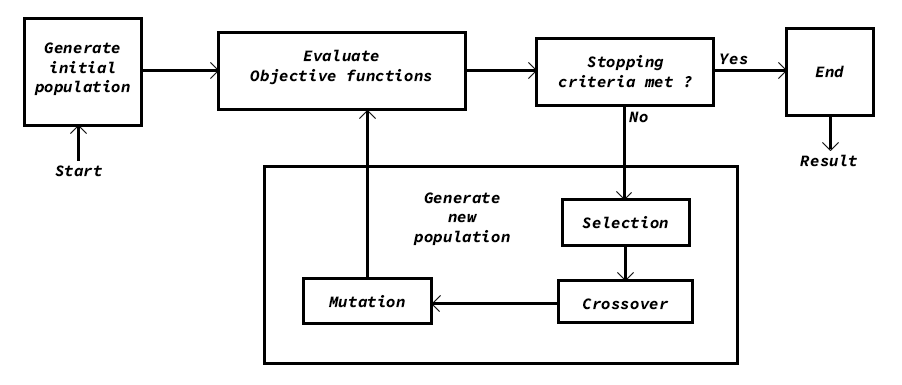
\includegraphics[width=0.8\textwidth]{img/ga_life_cycle.png}
    \caption{Ciclo de vida de un algoritmo genético}
    \label{figure:GA-Cycle}
\end{figure}

La lista anterior se muestra gráficamente en la Figura \ref{figure:GA-Cycle}, en
donde se puede apreciar más claramente como los operadores de selección, cruce y
mutación se engloban en una sola área que es la de la generación e integración
de nuevos individuos, éstos  también se evalúan para definir si el algoritmo ha
logrado alcanzar el punto de terminación, como
se explicó anteriormente estos nuevos individuos no se eliminan en caso de no
haber sido los ideales, sino que se comparan con los individuos originales y en
caso de ser mejores irán reemplazando a los peores con el fin de encaminar al
algoritmo a un punto especifico que se espera sea la solución idónea.

\section{Generación procedural de contenido}
\label{section:PCG}

El término "Generación procedural de contenido" (Procedural Content Generation o
PCG por sus siglas en inglés) denota la manera de crear contenido de manera
automática mediante algoritmos, en lugar de generar los mismos contenidos de
manera manual. %  Agrega referencias


La PCG es un sistema de generación de contenido utilizado desde finales de los
70s, inicialmente se utilizaba para generar los laberintos de algunos juegos
utilizando arte ASCII donde se denotaba la distribución de los cuartos y objetos
que se podían encontrar en juegos estilo \textit{"rogue"} 
o juegos que simulan %  Agrega referencias
un juego RPG de mesa, actualmente es ámbito de la generación de contenido ah
tomado varias variantes y cada vez más empresas toman un interés por el uso de
este tipo de herramientas de diseño, cabe remarcar que los diferentes ámbitos no
están del todo refinados sin embargo dada la información necesaria y aplicados a
aspectos específicos en el ciclo de desarrollo son capaces de crear los
contenidos que se requieran.

Mientras que la generación de contenido es un aspecto que se ha utilizado en
muchos ámbitos diferentes como en el fotografía, video, anuncios y arte digital, en
el área de videojuegos se maneja el uso de generación "procedural" de contenido
en donde procedural se define como el proceso computacional de una función
particular, en este caso lo que se busca con la generación procedural de
contenido es reducir el tiempo que toma generar contenidos de manera manual, la
siguiente sección explica más detalladamente como se utiliza esta mecánica en el
área de videojuegos.

\subsection{PCG en el ámbito de videojuegos}
\label{subsection:PCGInGames}

Dentro del ámbito de videojuegos la generación de contenido procedural es un
aspecto que ha tenido un gran impulso en tiempos recientes debido a que muchas
empresas de preocupan por sacar al mercado juegos de manera contínua, estos
mismos muchas veces en ciclos de desarrollos muy cortos, por lo mismo, se han buscado
diferentes maneras de reducir dichos problemas. Una herramienta útil que ha
surgido debido a esto es la generación procedural la cual permite reducir no
solo los tiempos de desarrollo, sino que también permite recudir el espacio de
memoria total de un juego en particular debido a que ya no es necesario tener
todos los archivos englobados en un solo lugar, sino que lo requerido se obtiene
de manera automática, de esta misma manera se les permite a las empresas reducir
el número de personal necesario y por tal reducir los costos de desarrollo.

La generación procedural de contenido tiene tres objetivos %% Referencias Según X la ..
principales:
\begin{itemize}
    \item Brindar apoyo a los creadores para poder crear contenido mas
    rápidamente.
    \item Utilizar la generación de contenido para crear juegos que logrean
    reaccionar en tiempo real a las acciones de los usuarios, cosa que en caso
    contrario tendría que encaminarse a escenarios específicos.
    \item Reducir el espacio en memoria tomado por el contenido generado.
\end{itemize}
Una cosa extra que brinda la generación procedural de contenido es permitir una
mayor creatividad al momento de generar.

\subsection{Áreas de interés de generación procedural}
\label{subsection:PCGAreasOfInterest}

La generación procedural de contenido es un sistema que se enfoca en diferentes
aspectos en el área del entretenimiento especialmente en el área de videojuegos,
estos aspectos pueden o no estar ligados unos con otros y además cabe mencionar
que no se enfocan primordialmente en la generación de "objetos" sino más bien en
la generación de recursos que pueden ser utilizados en el desarrollo de
videojuegos, la generación procedural se enfoca en seis puntos mostrados en la
Figura \ref{figure:pcg_areas}, cada uno se explica en un apartado iniciando con
el 'Diseño de niveles' en el capítulo \ref{subsection:LevelDesign}, la
generación de gráficos en el capítulo \ref{subsection:Visuals}, la creación de
audio en el capítulo \ref{subsection:Audio}, creación de narrativa o historias
en el capítulo \ref{subsection:Narrative}, diseño de reglas y mecánicas en el
capitulo \ref{subsection:rulesandmechanics} y la generación de juegos completos
explicada en el capítulo \ref{subsection:games}.

\begin{figure}
    \centering
    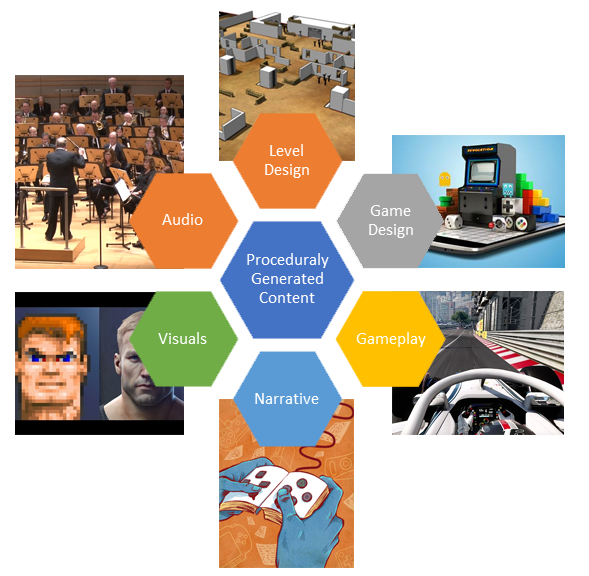
\includegraphics[width=0.6\textwidth]{img/pcg_areas.png}
    \caption{Áreas de PCG en videojuegos}
    \label{figure:pcg_areas}
\end{figure}

\subsection{Diseño de niveles}
\label{subsection:LevelDesign}

El área del desarrollo de niveles es una de las populares en PCG debido a que
los niveles son la parte esencial de un juego, debido a que es el área sobre la
cual un jugador puede interactuar, la representación de estas áreas pueden ser 
desde imágenes en 2D, simplemente con el alto y ancho de los objetos, hasta
elementos en 3D que abarquen también el grosor de los objetos.

Debido a que los niveles son esencialmente el área principal de interacción en
un videojuego, éstos deben de considerar los aspectos de funcionalidad y estética
para que exista una buena interacción y sea llamativo a los usuarios, de esta
manera se pueden crear áreas con tonos oscuros y ambiente tétrico para entregar
un nivel con temática de terror. La generación de niveles de juego es un tema
reciente en el ámbito de investigación debido a los elementos que se deben de
tener en cuenta sin embargo dentro del ámbito de videojuegos, es un elemento
comúnmente utilizado, algunos ejemplos recientes siendo Spelunky, Minecraft y
Disgaea. %% urls o referencias

Primero tenemos el juego de plataforma Spelunky desarrollado por Derek Yu, el
juego consta de múltiples niveles alrededor de cinco diferentes áreas, cada área
con un estilo diferente (niveles con hielo, lava, etc.) en este juego los niveles
que recorre el jugador son desarrollados de manera procedural por diferentes
algoritmos dependiendo el área en la que se encuentre el jugador.%% urls o referencias

El segundo ejemplo es un videojuego desarrollado por Markus Persson llamado %% urls o referencias
Minecraft, este juego consta de un área estilo caja de arena en donde el jugador
puede realizar las acciones que quiera, las estructuras están definidas en
manera de bloques con diferentes texturas y propiedades que el jugador puede
utilizar para construir diferentes cosas, la manera en cómo se utiliza la
generación de contenido es mediante la generación de todo un nivel al iniciar el
juego de tal manera que se utiliza una semilla de generación y se utiliza el
método \textit{Perlin Noise} 3D con interpolación lineal para generar los biomas,
elementos y entidades que conformaran el nivel, además de esto el área inicial
del juego no es la única área que puede ser recorrida durante la sesión de
juego, sino que el sistema utiliza una "semilla"(seed) que define la manera en
cómo está conformado el mapa, mientras más se va recorriendo del mapa las áreas
se van generando acorde a la semilla de manera infinita.

Finalmente tenemos el juego Disgaea desarrollado por Nippon Ichi Software, este %% urls o referencias
es un juego de estrategia por turnos en donde el objetivo es eliminar a todos
los enemigos en un mapa para continuar al siguiente, la manera en cómo se
utiliza la generación de contenido procedural es en una sección extra del juego
en donde se puede entrar a un arma para completar niveles gradualmente mas
difíciles para darle más poder a dicha arma, en esta parte los niveles que se
encuentra el jugador son generados proceduralmente tomando en cuenta las alturas
de las partes donde se puede caminar y la colocación de los enemigos en el mapa
\ref{figure:DisgaeaIW}, para la generación se toma en cuenta el nivel del arma y
su rareza, mientras más altos sean estos valores de igual manera los niveles
generados serán más difíciles.

\begin{figure}
    \centering
    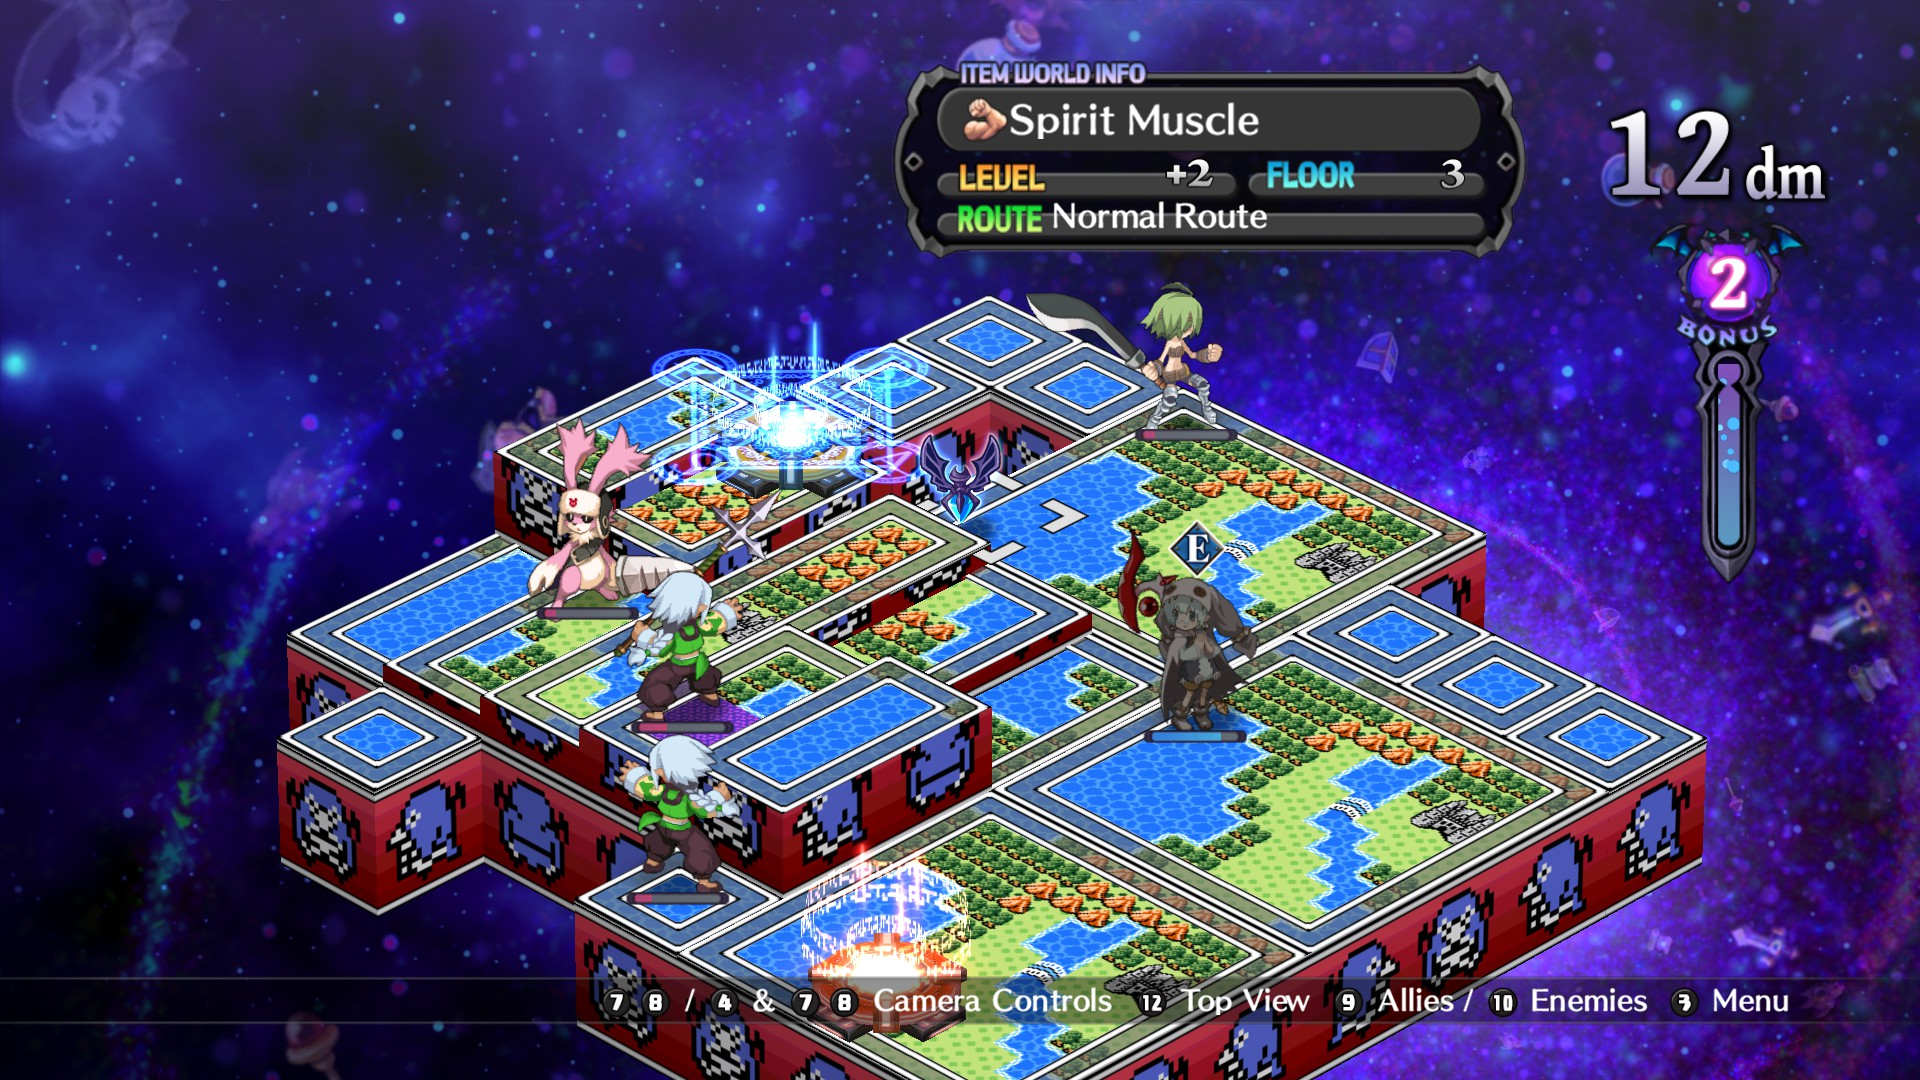
\includegraphics[width=1.0\textwidth]{img/DisgaeaIW.png}
    \caption{Nivel generado en el juego Disgaea}
    \label{figure:DisgaeaIW}
\end{figure}

\subsection{Gráficos}
\label{subsection:Visuals}

El área de desarrollo de gráficos se encarga principalmente de generar las
representaciones visuales de los juegos debido a que la mayor parte de los
juegos llevan una parte visual a menos que no se requiera, es necesario generar
una imagen que denote lo que se quiere dar a entender en un juego, de esta
manera se le brinda al jugador un nivel más de inmersión en la situación,
mediante el uso de paletas de colores o imágenes en pantalla que puedan
representar mejor las situaciones que se presentan.

El ámbito de generación de gráficos ha sido uno de los más explotados debido a
que es posible generar gráficos que van desde simples representaciones de 8 bits a
representaciones foto realísticas de los eventos u objetos presentes en un
juego. Tal es el caso explicado en el paper de Risi S. et al.\cite{Risi2012} en
donde utilizan una red de producción de patrones composicionales (CPPN por sus
siglas en inglés) la cual es una variante de las redes neuronales artificiales
(ANN) regulares, utilizando esta red se buscó modificar un círculo de tal manera
que la resultante de tal modificación creara un patrón en forma de una flor, de
igual manera la forma de crear diversidad en los tipos de flores generadas fue
mediante el uso de la neuro evolución de topologías aumentativas (NEAT) mediante
el cual las redes generadas se alteraban mediante la modificación de conexiones
entre neuronas y la adición de nuevos nodos de tal manera que se buscaba un
nivel adecuado de complejidad para las redes que generaron diferentes tipos de
patrones de flores.

Mientras que un segundo artículo escrito por Erin J. et al.\cite{Hastings2009} en
el cual presentan un nuevo algoritmo de generación de contenido llamado
neuro evolución de topologías aumentativas para generación de contenido (cgNEAT)
el cual se encarga de generar contendió gráfico y contenido del juego de acuerdo
a las preferencias de un jugador mientras el juego está en ejecución, para la
evaluación del contenido generado se desarrolló un juego multijugador en línea
llamado \textit{Galactic Arms Race} en el cual la cgNEAT se encarga de generar
contenido para todos los jugadores y ellos eran quienes proveían la
retroalimentación del funcionamiento del algoritmo.

\subsection{Audio}
\label{subsection:Audio}

El ámbito de generación de audio en videojuegos se puede considerar como un
punto opcional dependiendo del juego que se esté desarrollando sin embargo el
audio juega un papel importante en la experiencia que se le brinda a un jugador
dentro del juego debido a que mediante el uso de componentes sonoros se pueden
influir las emociones que se quieren mostrar en lugares específicos, desde cosas
simples como el uso de sonidos de objetos como escuchar un teclado siendo
utilizado hasta la utilización de pistas de audio en áreas o momentos clave del
juego para demostrar momentos dramáticos, tristes o de acción. 

Cabe mencionar que es posible utilizar instrumentos musicales o la
implementación de orquestas para de igual manera generar estos ambientes sin
embargo algunos utilizan este tipo de generación para crear pistas que sean
capaces de adaptarse a los sucesos que transcurren en el momento para el
concepto de generación procedural de audio puede ser inclusive el uso de
elementos en un entorno virtual que generen algún sonido cuando son
interactuados \cite{garner2014sonic}, algunos ejemplos de adaptabilidad de audio
de acuerdo a los eventos en el momento es el caso del juego \textit{Fire emblem
Fates}, este es un juego de estrategia por turnos en donde la adaptabilidad de
audio se da en transiciones de vista del mapa y combate de unidades, en este
caso el audio de la vista del mapa tiene un cierto nivel de \textit{tempo}
mientras que en momento que se entra a un combate entre dos unidades el
\textit{tempo} del audio cambia mientras se está en esta escena de combate.

Existen también investigaciones académicas de como combinar la generación de
niveles con la generación de audio, tal es el caso de \textit{Sonancia}
desarrollado por Phil Lopez et al. \cite{lopes2015sonancia}, en este paper los
autores proponen una metodología que permitirá a un sistema generador de niveles
seleccionar pistas de audio o sonidos que vallan de acuerdo a un tema específico,
en este caso los autores colocaron una lista de pistas y mediante un generador
crearon un entorno 2D que simulaba una mansión, el propósito fue el de crear un
juego de terror/suspenso y que las habitaciones tuvieran un audio diferente y
que al acercarse a la división entre una y otra el audio de la habitación
adyacente fuese subiendo el volumen conforme más se adentraba y el audio de la
habitación anterior se dejará de escuchar lentamente, el sistema es capaz de
generar los niveles y asignar los sonidos necesarios sin embargo tiene la
limitante de que se debe de proporcionar el listado de pistas de audio debido a
que aún no tiene la capacidad de generar audio por cuenta propia sin embargo es
otro buen ejemplo de cómo combinar áreas de generación de contenido.

Otro caso de estudio es el del juego \textit{Audio Surf} desarrollada en 2008 por
Fitterer, la manera en cómo funciona es que mediante el uso de archivos de audio
de alguna canción para generar niveles estilo pista de carreras que el usuario
recorre al momento de jugar, como este existen varios otros juegos que utilizan
mecánicas de PCG para generar los niveles a jugar por los participantes.

Finalmente tenemos \textit{Mezzo} desarrollado por Daniel B. este artículo muestra
un programa de computadora del mismo nombre diseñado con el fin de generar
música de la era romántica que puede ser utilizada en juegos de computadora, el
software fue desarrollado con el propósito de poder darle más expresividad a
eventos que ocurren en juegos de computadora, esto es mediante el uso de los
elementos presentes en la escena como las partes que conforman la pieza musical,
para esto sus acciones son traducidas como diferentes cantidades de tension
armónica lo cual permite que la pieza musical corresponda al estado del juego
así como a las acciones que realizan los personajes.

\subsection{Narrativa}
\label{subsection:Narrative}

El ámbito de generación de narrativa en videojuegos se encarga de manera básica
de generar historias que tengan sentido y sean entretenidas, el uso de PCG para
el ámbito de narrativa se ha tomado de diferentes ángulos, el primero es
sencillamente crear la historia del lugar en donde se desarrollan las cosas,
esto es generar toda la historia desde un punto especifico y así crear una
"línea" de acción que un jugador deberá seguir, mientras que otro de los
aspectos es la generación de historia que se adapte a las acciones del jugador,
esto es, que a medida que el jugador progrese en un juego realizando acciones
especificas el juego adapte la historia a generar de acuerdo a dichas acciones.

Algunos ejemplos de este ámbito de generación se muestran en el juego
\textit{Facade} y el sistema \textit{Versu}, el primero que se explicara es el
juego de Facade, Facade es un juego desarrollado por Michael Mateas y Andrew
Stern \cite{mateas2003faccade} que intenta crear un juego estilo novela visual
en donde las acciones del jugador tengan influencia en los eventos que ocurren
en el juego, el juego introduce al personaje del jugador como un amigo de una
pareja de casados, no se cuenta con un objetivo específico más que el de
completar la historia, sin embargo, el juego provee de acciones y respuestas que
el personaje puede expresar a la pareja, estas mismas tienen influenciaran
directamente el cómo se desarrollará la historia, el juego se diseñó con el
propósito de que el jugador lo repita múltiples veces con el fin de descubrir
como las diferentes decisiones cambiaran el desenlace de la historia. 

Finalmente \textit{Versu} es una aplicación desarrollado por Richard Evans y
Emily Short \cite{evans2013versu} es juego se encarga de generar simulaciones en
base a líneas de texto que denotan acciones que un conjunto de personajes no
jugables (NPC) realizan en determinados escenarios, el juego permite que a una
persona se le asigne un personaje del juego y controle las acciones que
realizara, mientras que los NPC restantes responderán de manera autónoma
mientras el juego continua, este sistema de generación de narrativa inicio como
un proyecto académico y después paso a ser utilizado de manera comercial, además
de ser la base para el desarrollo de otros juegos de estilo similar.

\subsection{Reglas y Mecánicas}
\label{subsection:rulesandmechanics}

Las reglas y mecánicas de un juego proveen un framework en el cual el
jugador puede realizar acciones y el cómo debe de influenciarlas hacia un
objetivo final, las reglas y mecánicas de un juego pueden variar dependiendo del
tipo de juego que se trate, por ejemplo, en juegos de estilo plataforma la regla
de terminación puede ser simplemente llegar hasta cierto punto del nivel
mientras que las mecánicas pueden incluir saltar, correr o agacharse, este
conjunto de reglas permite que el jugador no realice acciones no previstas por
los programadores y de tal forma limita a un jugador a cierta cantidad de
acciones y consecuentes posibles las cuales deberá de aprovechar de diferentes
maneras para continuar.

Mientras que el uso de reglas permite tener un juego más balanceado algunas
ocasiones el cambiar el conjunto de reglas permite crear diferentes tipos de
juegos, tomando el ejemplo anterior es posible que un juego de plataformas se le
permita a un jugador volar en un nivel lo cual provocaría que las mecánicas se
requieran acomodar a esta nueva habilidad y de igual manera los niveles de un
juego se tengan que re-imaginar de tal modo que ahora se pueda utilizar en
ciertas o se coloquen lugares que solo se pueden acceder con esa habilidad por
ejemplo la transición de reglas y mecánicas entre los juegos Super Mario Bros.
(Nintendo, 1985) y Super Mario World (Nintendo, 1990). %Referencias

Para la evaluación de la generación de mecánicas y reglas de un juego existen
diferentes métodos a utilizar, el primero se basa en el balance de las reglas es
decir en caso de ser un juego para dos o más jugadores el objetivo de evaluar
sería que todos los jugadores tengan las mismas probabilidades de ganar
utilizando las mecánicas del mismo juego, mientras que otra manera de evaluar
seria mediante la facilidad que tienen las mecánicas de ser aprendidas por los
jugadores.

En cuanto a ejemplos de este tipo de generación se encuentran algunas
investigaciones académicas tales como la de Ludi \cite{Browne2010}, Ludi es un
sistema desarrollado por Cameron Browne y Frederic Maire, este sistema se
utiliza para evolucionar comandos que definen las reglas de un juego en
particular a crear, el algoritmo evolutivo se encarga de evolucionar las reglas
manteniéndolas dentro de un cierto rango de métricas que establecen un buen
patrón para juegos de tablero tales como tales como la complejidad del juego o
la simplicidad de las reglas, un juego de mesa diseñado mediante el uso de este
sistema se llama Yavalath, una vista rápida del juego se puede apreciar en la
figura \ref{figure:Yavalath}, este juego puede tener un mínimo de 2 y un máximo
de 3 jugadores, las reglas son que en base a turnos cada jugador coloca una
ficha de su color en cualquier punto no ocupado del tablero, el objetivo es
lograr formar una línea de 4 fichas del mismo color, pero la regla es que al
formar una línea de 3 fichas se pierde el juego de manera automática, de esta
manera el juego se basa en forzar jugadas del oponente que permitan que alguno
tenga más "control" de los eventos que ocurrirán. 

Un segundo caso fue escrito por Togelius et al. \cite{Togelius2008}, este uno de
los primeros ejemplos del uso de computación evolutiva para la generación de
reglas para juegos, en este paper se evoluciona un conjunto de reglas de tal
manera que un conjunto de agentes que participaran en el juego logren tener un
mejor entendimiento de como funciona el juego, la manera de evaluar que tan
entendibles son las reglas fue a través de varias sesiones simuladas de los
agentes, en este caso se procuró utilizar reglas sencillas que simularan un
juego estilo pac-man en donde los agentes deberían de colectar círculos para
poder obtener una mejor puntuación.

Finalmente, un último caso es el de Nielsen et al. \cite{Nielsen2015} esos
autores programaron un sistema capaz de representar las reglas de un videojuego
utilizando video game description language en donde juegos estilo 2d se
representan como mapas en base a caracteres y utilizaron ASP para verificar que
los niveles podían ser jugados (se podían cumplir las condiciones de victoria).

\begin{figure}
    \centering
    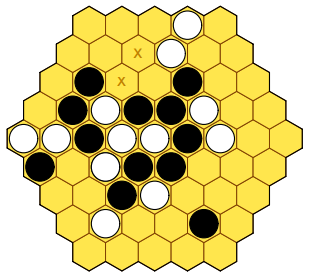
\includegraphics[width=0.6\textwidth]{img/Yavalath.png}
    \caption{Ejemplo de un juego en progreso en el juego de Yavalath}
    \label{figure:Yavalath}
\end{figure}

\subsection{Juegos}
\label{subsection:games}

Mientras que las facetas de generación anteriores se han enfocado en aspectos
específicos de juegos mientras que en este aspecto en particular se toma un
enfoque global, esto es desde la generación de partes visuales hasta la 
generación de bandas sonoras, esto demuestra como todos los aspectos de un
juego se relacionan unos con otros, un ejemplo de esta relación seria tomar un
juego en particular y agregar acciones que originalmente no existían, para poder
agregar estas acciones se debe de considerar el aspecto visual, es decir el como
deberá de representarse visualmente tal acción, aspectos de sonidos en caso de
que una acción requiera de algún efecto de sonido que represente tal acción,
utilizando el ejemplo de agregar la mecánica de volar, el aspecto visual se
representaría en un cambio visible en el personaje controlado, por ejemplo,
dibujar alas y que se vea una animación de movimiento al volar, en el caso del
aspecto del sonido el aleteo o movimiento generado por dichas alas al estar
volando puede tener un sonido único para identificarlo.

Para este caso existen diferentes maneras de intentar generar juegos nuevos, tal
es el caso de Game-O-Matic \cite{treanor2012game}, Game-O-Matic es una
herramienta de generación enfocada a la generación de juegos que representan
ideas, en este sistema se utiliza un sistema de sustantivos unidos mediante
verbos que son ingresados al sistema como datos de entrada, estos datos son
procesados y se logra generar un juego simple estilo arcade que logre
representar un mapa conceptual generado mediante los valores de entrada. 

Otra investigación realizada por Nelson et al. \cite{Nelson2008}, para este
sistema los autores proponen un sistema parecido al de Game-O-Matic explicado
anteriormente, sin embargo, en este caso el sistema está basado en sprites que
representan entidades del juego, lo que se asigna como valor de entrada es
restricciones que definen la interacción de los sprites en pantalla, las
restricciones son procesadas mediante una red semántica y una base de datos de
léxico, este proceso logra generar juegos que cumplan las restricciones
estipuladas, en este caso los juegos generados tienen mecánicas estilo WarioWare
en donde los juegos tienen una regla de victoria sencilla que hace los juegos
relativamente cortos. 

Finalmente, uno de los mejores generadores de juegos lleva en nombre
de ANGELINA \cite{cook2011multi} %(Ref ANGELINA num135-137) 
\footnote{De acuerdo al autor: "A Novel Game-Evolving Labrat I've Named
ANGELINA"}, ANGELINA es un sistema de generación de juegos diseñado
originalmente en 2011 y que ha recibido modificaciones desde entonces, la base
del generador es el uso de un sistema evolutivo que se encarga de evolucionar
las reglas, los terrenos, los personajes y demás conjuntos con respecto unos de
otros de una manera orquestada, se encarga no solo de evolucionar la
información visual de los componentes sino también de asignar sus locaciones en
un campo de trabajo que representa un juego, además de esto es capaz de
seleccionar elementos musicales relevantes al tema de los mapas generados o de
la faceta emocional presente en el juego además de crear asignarle un nombre a
los juegos que logra crear, inicialmente el sistema era capaz de generar niveles
de plataforma en 2D, pero actualmente es capaz de generar niveles de temática de
aventura en entornos 3D.

Los anteriores generadores a pesar de no ser perfectos han permitido dar un gran
paso en la generación de contenido o más bien en la generación de juegos, sin
embargo aún falta controlar aspectos que permitan que las generaciones de tal
contenido logren involucrar todos los aspectos de la generación de contenido,
esto podría darse mediante el uso de múltiples agentes que contantemente evalúen
los aspectos generados pero que al mismo tiempo logren comunicarse unos con
otros y poder evaluar los juegos generados de manera más amplia.

\section{Jugabilidad}
\label{section:playability}

La jugabilidad es un término utilizado principalmente en el área del análisis y
diseño de videojuegos y es utilizado principalmente como medida de calidad para
la experiencia de un usuario para con el juego mediante las mecánicas o manera
en cómo se tiene una interacción jugador-videojuego y el diseño como tal del mismo.

De igual manera diferentes autores definen el concepto como un conjunto de
propiedades que definen la experiencia que logra tener un jugador en un juego
determinado según al sistema de juego que se provee.

\begin{figure}
    \centering
    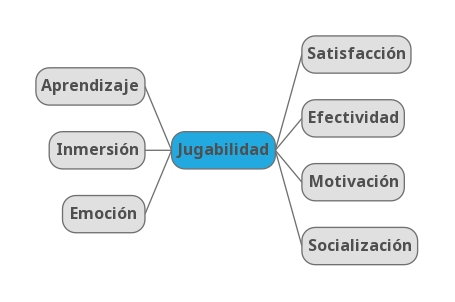
\includegraphics[width=0.7\textwidth]{img/playabilityv2.png}
    \caption{Puntos de evaluación de jugabilidad}
    \label{figure:playability}
\end{figure}

La figura \ref{figure:playability} muestra un diagrama de áreas y conceptos que
califican el nivel de jugabilidad de una aplicación o juego, estos mismos se
pueden definir como sigue:

\begin{itemize}
    \item Satisfacción: El grado en el que un juego logra agradar o complacer a
    un usuario.
    \item Aprendizaje: El grado con el cual un usuario es capaz de comprender
    las mecánicas de un juego y es capaz de interactuar fácilmente con el mismo.
    \item Efectividad: Este demuestra la cantidad de recursos y el tiempo
    utilizados para poder envolver a un usuario y lograr que se divierta.
    \item Inmersión: El grado con el cual se logra envolver a un usuario con los
    eventos que transcurren en el juego, es decir que tanto se logra hacer que
    se integre o muestre empatía por los eventos del juego.
    \item Motivación: Esta define la capacidad que tiene un juego a motivar a un
    usuario a continuar con los retos o eventos del juego, esto generalmente se
    da por mecánicas que dan un sentimiento de recompensa o simplemente por la
    inmersión lograda.
    \item Emoción: Es el grado con el cual se logra una inmersión en el usuario
    de tal manera que es capaz de reaccionar de manera involuntaria a estímulos
    presentados en el juego, esto puede ser desde una risa por algún evento que
    ocurre hasta saltos involuntarios por susto en juegos de terror.
    \item Socialización: Este es el grado con el cual se logra que un usuario
    entable relaciones con personas que no conoce, en juegos de multijugador
    masivo en línea("Massive-Multiplayer Online" - MMO por sus siglas en ingles)
    existen eventos en los cuales se le pide a los usuarios que construyan
    equipos para completar niveles en el juego, existen otros juegos de
    multijugador local en los que varias personas compiten para ganar, y en
    ambos casos se puede presentar que de los sucesos presentados se puedan
    crear amistades entre jugadores.\cite{sanchez2009playability}
\end{itemize}

Por otro lado, existe un conjunto de facetas que engloban varios atributos de la
jugabilidad que permiten relacionar dichos atributos, para estas facetas se
toman los siguientes grupos:

\begin{itemize}
    \item Jugabilidad intrínseca: Engloba el diseño y mecánicas del juego
    enfocándose en las reglas y objetivos establecidos, define el cómo se
    proyectan estos puntos al jugador.
    \item Jugabilidad mecánica: Se enfoca en parte funcional del juego y en los
    comportamientos de los personajes, se basa en el diseño del motor del juego.
    \item Jugabilidad interactiva: Se enfoca más en la relación usuario-juego,
    tomando en cuenta el cómo se presenta la interfaz de usuario y los controles.
    \item Jugabilidad artística: En este punto se engloban los puntos de
    gráficos y sonido, es decir que tan bien es visualmente lo que se presenta y
    el tipo de ambientación que se crea al combinar efectos visuales, música y gráficos.
    \item Jugabilidad perceptiva: Este punto trata de cuantificar la manera en
    como una persona percibe los elementos mostrados en el juego, este es un
    calculo subjetivo.
    \item Jugabilidad interpersonal: Al igual que el punto anterior es un
    concepto subjetivo, sin embargo, este se enfoca en las percepciones que se
    generan al jugar en un grupo.
\end{itemize}

\section{Open-Ended Evolution}
\label{section:open-ended_Evolution}

El termino Open-Ended Evolution (OEE) es el nombre que se le da a una variante
del algoritmo de evolución genética, este algoritmo difiere de los objetivos
predefinidos de un algoritmo genético en el cual el objetivo principal de un GA
es el de llegar o aproximarse a un valor o conjunto de valores que logren
solucionar un problema determinado, en el caso de OEE este no es el caso sino
que lo que hace el algoritmo es seguir evolucionando y creando diversidad en la
población cada vez más compleja no solo dentro de los límites de evolución de un
elemento sino comenzar a crear nuevas \textit{"especies"} de soluciones.

Una explicación más clara es presentada en un paper por T. Taylor et
al.\cite{Taylor2016}, en este paper se define OEE como un sistema capaz de
novedad después de un punto en la evolución en donde el estado del grupo o
población no cambia en lugar de converger hacia un estado casi estable.

La manera en cómo se definirá el uso de OEE que se utilizara en este proyecto es
simplemente un proceso de evolución genética capaz de encapsular procesos de
evolución similares capaces de incrementar en número según la complejidad a la que
las entidades generadas logren llegar.

\chapter{Estado del arte}
\label{chapter:related-work}

Este capítulo se enfoca en mostrar los diferentes trabajaos que permitirán
comprender mejor la problemática que se quiere resolver, así como los diferentes
enfoques que se le han dado para poder resolverlo.

\section{Competencia IEEE CoG}
\label{section:ieeecog}

Como se demuestra en el artículo presentado por J. Renz et al.\cite{Renz2016} la
competencia de Angry Birds utilizando inteligencia artificial se realiza de
manera anual desde el año 2012 iniciando en la conferencia dentro del marco de
la AAAI (Association for the Advancement of Artificial Intelligence), en este
artículo se explica la primera línea de competencia que consta de desarrollar
agentes que sean capaces de solucionar niveles del juego de tal manera que se
asemeje a la manera en cómo jugaría una persona real, se explica el estado del
arte el cual consta de previos competidores y de cómo han logrado realizar sus
agentes para el juego, de igual manera se explica la nueva línea de competencia
que consta de utilizar el mismo conjunto de niveles y permitir que los agentes
compitan para ver cual logra resolver más rápido el conjunto de niveles.

Posteriormente en un artículo elaborado por M. Stephenson et
al.\cite{Stephenson2018The2A} se explica detalladamente como es que el juego se
conecta en una arquitectura cliente-servidor y como es que se adapta la
arquitectura para que los agentes utilizados puedan obtener datos del juego para
poder realizar los cálculos pertinentes, en este mismo artículo se presenta
información de la segunda línea de competencia llamada competencia de generación
de niveles de AIBIRDS la cual se comenzó a realizar desde el año 2016, en esta
versión de la competencia los generadores deben de cumplir con el propósito de
crear noveles que sean creativos, divertidos, estables en cuanto a la gravedad
del juego y posibles de ser solucionados, además de esto se debe de tener en
consideración realizar niveles que sean desafiantes a los jugadores, como el
juego no es open source los niveles se generan en una versión clon del juego que
cuenta con las mismas mecánicas.

Un segundo artículo escrito por M. Stephenson et al.\cite{Stephenson2018} se
presenta una versión más actualizada de las reglas de la competencia, en este
artículo se establece el uso de un archivo proporcionado por los organizadores,
este archivo cuenta con 4 líneas en las cuales se establece las condiciones que
los niveles generados deberán de cumplir, la información proporciona en el
archivo es la cantidad de niveles que se deberán de generar, las piezas no
permitidas en un nivel, así como las combinaciones que se deberán de evitar, la
cantidad de puercos a colocar en un nivel y por último el tiempo límite para
terminar los niveles, en el caso de los tipos de materiales prohibidos se
entrega una lista que especifica que piezas con que material no se puede
colocar, en el caso de los puercos se entrega un rango numérico en el cual se
especifica la cantidad mínima y máxima a colocar, en cuanto a los valores de
niveles y tiempo límite se entregan como valores numéricos enteros, sin embargo
los valores que se entregan generalmente son 5 para la cantidad de niveles y 30
en la cantidad de minutos que puede durar el generador.

\section{Algoritmos de búsqueda}
\label{section:search-based}

L. Ferreira et al.\cite{Ferreira2014} presentaron un sistema de generación de
niveles mediante el uso de algoritmos genéticos, en el sistema se propone la
definición de un individuo como una lista de elementos que se acomodaran en
forma de torre, el sistema propuesto utiliza las piezas base del juego y se
agregaron 4 elementos compuestos, los niveles se definen como un área de trabajo
con tres posiciones donde las torres podrán ser generadas a base de las piezas
en la lista principal, las piezas irregulares tales como los dos diferentes
tipos de triángulos son tomados en cuenta únicamente en la última posición de
las torres.

Una herramienta de generación de niveles basado en el uso de patrones de
generación es propuesto por Y. Jiang et al.\cite{Jiang2017}, en este paper los
autores proponen el uso de patrones predefinidos de generación de estructuras
basadas en el alfabeto americano, valores numéricos, símbolos, así como el
ordenamiento de estos en base a patrones de frases o palabras predefinidas que
pueden ser utilizadas, utilizando estos patrones se generan niveles en donde se
muestran frases divertidas o motivacionales que serían jugados por personas para
evaluarlos, debido a la manera de acomodo de bloques utilizada en este paper el
problema de que los niveles sean estables se eliminaba y simplemente se utiliza
el sistema para cumplir los dos objetivos restantes los cuales son que los
niveles sean jugables y entretenidos, mientras que la manera final de evaluar la
funcionalidad del generador se basaba la re-jugabilidad, la legibilidad del texto
así como de la dificultad de los niveles, para esto los autores se apoyaron de
10 personas con cierto grado de comprensión del idioma inglés, de esta manera en
caso de que los textos fueran difíciles de comprender, la dificultad fuera
demasiado alta o generara un interés por repetir el nivel los participantes
serían los encargados de proporcionar estos resultados.

Para la adaptabilidad de los niveles basados en los resultados de la función de
aptitud M. Kaidan et al.\cite{Kaidan2015} proponen una medición basada en la
habilidad de un jugador en un nivel, la evaluación de la habilidad está dada por
el puntaje obtenido durante el juego, en el juego de angry birds el puntaje de
un jugador está ligado a la cantidad de destrucción de estructuras lograda y la
cantidad de aves que no se utilizaron para completar el nivel, en este caso el
paper se apoyaba de la función de aptitud de L. Ferreira et
al.\cite{Ferreira2014} para la distribución de los puercos en un nivel y se
adaptaba la función para modificar la cantidad de puercos colocados de acuerdo a
la facilidad con la que se lograba resolver el nivel, de esta manera el sistema
generaba un conjunto de niveles para que una persona los solucionara y basándose
en los resultados de los niveles se generaba el siguiente conjunto para
resolver, de tal manera que el sistema requería que una persona evaluara los
niveles cada generación para que el sistema generara niveles más desafiantes
para esa persona.

Otro generador propone el uso de un selector de dificultad como parámetro de
entrada de un algoritmo genético para la generación de niveles con elementos
predefinidos, en este paper M. Kaidan et al.\cite{Kaidan2016} utilizan una
versión extendida del Algebra de Intervalo Temporal de Allen (Allen's Temporal
Interval Algebra)\cite{ALLEN1990} para calcular área mínima delimitadora
(Minimum Bounding Rectangle) de cada elemento del juego para realizar cálculos
de posición más exactos al momento de obtener resultados, utilizando estas
mecánicas proponen evaluar la relación de movimiento después de que un ave a
impactado en alguna de las piezas del nivel.

Otros investigadores proponen utilizar sistemas de generación que no incluyan
limitantes en las estructuras a fin de permitir una evolución general mas
"libre" tal es el caso del paper desarrollado por L. Calle et al.
\cite{Calle2019} en donde utilizan un sistema de generación que ignora la
necesidad de crear estructuras siguiendo patrones o simetría, en este paper se
busca utilizar un espacio de búsqueda relativamente pequeño para ahorrar tiempo
de procesamiento, además de esto utilizan una aplicación de código libre llamada
Box2D (https://box2d.org) sobre la cual está basado el código del juego de Angry
Birds y permite realizar simulaciones de manera más rápida debido a que solo se
calcula la estabilidad de las estructuras para el valor de fitness de los
individuos, sin embargo, debido que el sistema de generación no está encaminado
por patrones las estructuras finales generadas carecen de llamatividad visual,
cabe mencionar que este trabajo se utilizó como base para el desarrollo del
proyecto actual, algunas de las ideas tuvieron origen en este trabajo para ser
modificadas y adaptadas en nuestra propuesta.

\section{Agentes para jugar}
\label{section:others}

De igual manera varios autores toman la ruta de programación de agentes que sean
capaces de solucionar los niveles presentados en el juego, de estos se hacen
mención algunos.

Dentro de la competencia de diseño de agentes el objetivo es que el agente sea
capaz de solucionar los niveles utilizando las mecánicas de gravedad y colisión
del juego, por tal manera F. Calimeri et al. \cite{Calimeri2016} propones el uso
de una forma de programación declarativa llamada Answer Set Programming (ASP por
sus siglas en inglés) dicha mecánica está orientada hacia algoritmos de búsqueda
difíciles, en este caso utilizan ASP para analizar el campo de juego que
involucra los bloques utilizados en las estructuras y los puercos estacionados
en ellas, de esta manera ASP tratara de identificar el daño que puede ser
causado, así como el movimiento resultante de los bloques en base a la gravedad
del juego al momento de disparar un ave en un cierto angulo con determinada
fuerza, en base a esto se determina el siguiente tiro a realizar para poder
completar el nivel. 

Diferentes autores han utilizado diferentes técnicas para la generación de
contenido, algunas utilizando computación evolutiva y algunas otras simplemente
a base de algoritmos de búsqueda, de estos mismos los más relevantes se les hace
mención: G. Smith et al.\cite{Smith2009} proponen un software de generación de
niveles estilo juego de plataformas mediante el uso de un software aplicando
inteligencia artificial, en este software se le permite a un usuario seleccionar
la altura del punto de inicio y punto final de un nivel en particular y el
sistema trata de llenar el espacio restante con plataformas que permitan que el
nivel se pueda completar, el sistema se basa en una medición de pulsos en los
cuales una persona podría realizar una acción determinada para avanzar a la
siguiente sección.

\chapter{Propuesta del proyecto}
\label{chapter:proposed-method}

Este capítulo describe los componentes que integran el método propuesto, así
cómo la manera en cómo estos componentes proveen de apoyo al sistema final, este
capítulo está dividido en dos secciones la primera siendo la sección
\ref{section:used-method} en donde se explican los conceptos propuestos y
utilizados en el proyecto, esta sección se divide en varias subsecciones en
donde se explican partes de la propuesta y el cómo permitirán que el sistema
generado cumpla con los objetivos requeridos, la segunda sección
\ref{section:previous-proposed-methods} explica ideas y conceptos que se
propusieron a lo largo del desarrollo y el cómo estos ayudarían a mejorar el
sistema generado.

\section{Propuesta utilizada}
\label{section:used-method}

La propuesta final utilizada en el proyecto está basada en el uso de varias
técnicas para la generación de los compuestos y subsecuentemente los niveles
para el juego de Angry Birds, la base de todo el proyecto está en el uso de un
algoritmo genético para evolucionar los individuos, esto se explica más a
detalle en la sección \ref{subsection:generate-levels-using-GA}

\subsection{Generar compuestos de piezas base}
\label{subsection:generate-composites}

El videojuego de Angry Birds cuenta con un total de 11 diferentes tipos de
bloques, además de 2 grupos de objetos siendo estos cajas de explosivos y los
puercos que pueden ser colocados en el nivel, además de esto cuenta con
plataformas que pueden ser agregadas y rotadas para establecer plataformas en
donde colocar más bloques, de estos solo utilizaremos las 11 piezas básicas
mostradas en la Figura \ref{figure:game-basic-blocks} y los puercos para generar
niveles.

Las piezas básicas no pueden ser modificadas, tampoco es posible agregar nuevos
bloques al código debido a que la competencia solo utiliza las piezas regulares,
para poder librar esta restricción se generarán compuestos con las piezas base,
estos compuestos pueden estar formados de 1, 2 o más bloques básicos, estos
grupos se utilizarán para generar las estructuras que se colocaran en los niveles.

\begin{figure}
  \centering
  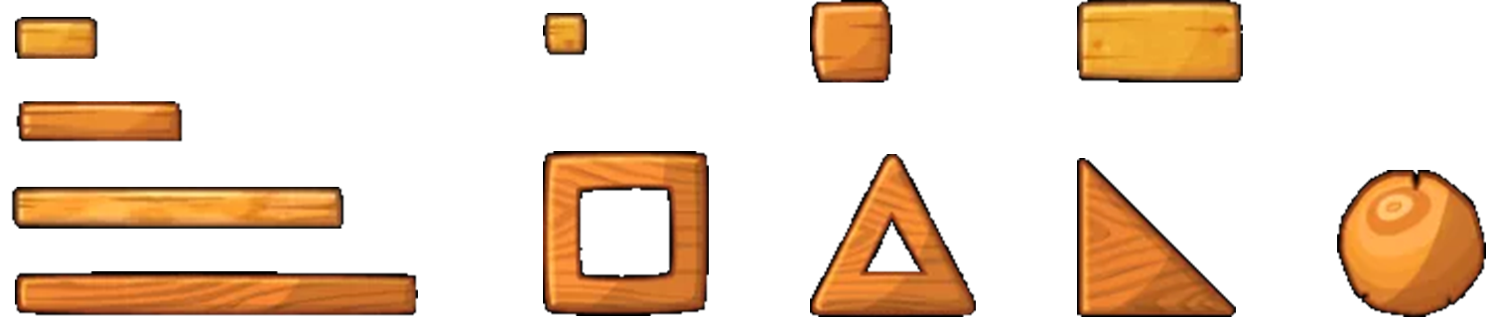
\includegraphics[width=1.0\textwidth]{img/list_pieces.png}
  \caption{Piezas básicas del juego angry birds}
  \label{figure:game-basic-blocks}
\end{figure}

La manera propuesta para generar estos conjuntos es mediante el uso de los
valores de alto y ancho de las piezas para poder definir los bordes de las
mismas, de esta manera al momento de querer unir dos o más piezas para formar un
conjunto la medida del conjunto se calculará buscando el punto más alto, más
bajo, así como las posiciones más a la derecha e izquierda teniendo ambas piezas
unidas, un ejemplo de la unión de cuatro piezas se muestra en la Figura
\ref{figure:bounding-box-calculation} en donde cuatro piezas se colocan una
sobre otra para formar un objeto cuadrado. Para poder agregar las piezas cómo
un conjunto se buscan los puntos más alejados, una vez que se ha calculado el
alto y ancho del conjunto se procede a encontrar el punto central del mismo,
desde este punto se calcula la distancia en \textit{x} y \textit{y} hacia los
centros de cada una de las piezas del conjunto, estos valores de centros se
agregan utilizando una estructura de diccionario para poder generar los objetos requeridos al
momento de crear a los individuos antes de iniciar las generaciones.

\begin{figure}
  \centering
  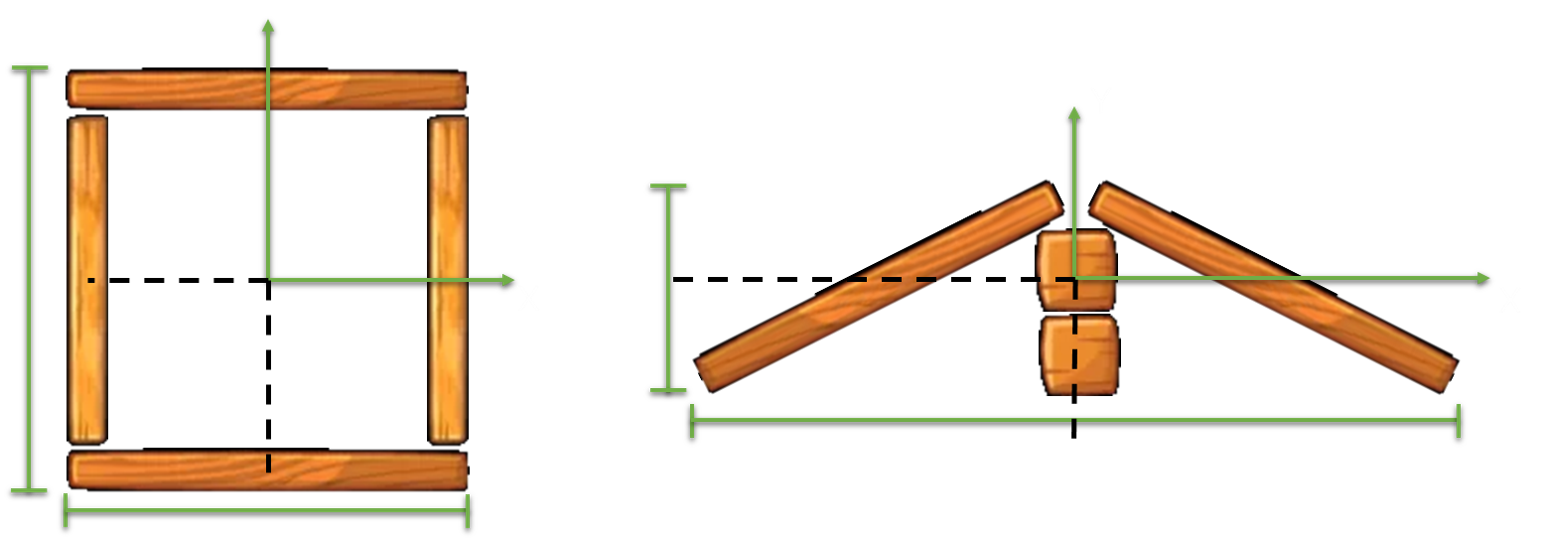
\includegraphics[width=1.0\textwidth]{img/bounding_box_calculation.png}
  \caption{Cálculo de bordes de un conjunto}
  \label{figure:bounding-box-calculation}
\end{figure}

Debido a que los conjuntos son creados antes de la ejecución del algoritmo se
permite que el algoritmo se base únicamente manteniendo los apuntadores a las
composiciones de piezas y solo trabaja con estas mediante las operaciones
genéticas del propio algoritmo, esto permitirá que el algoritmo utilice menos
tiempo identificando posibles composiciones.

Utilizando esta manera de generar los compuestos se utiliza un
algoritmo orientado a objetos, para poder acomodar los elementos y crear los objetos
requeridos según sean necesarios, esto se explica más detalladamente en la
sección \ref{subsection:classorientedidea}.

\subsection{Generación de compuestos mediante objetos de clase}
\label{subsection:classorientedidea}

Para mantener un control de los compuestos, principalmente de las piezas
individuales, se propuso la una jerarquía de clases con
herencia, en donde una clase base contendrá los métodos que las clases derivadas
para obtener valores específicos cuando las piezas requieran,
principalmente estos métodos se encargan de calcular las esquinas de las piezas
particulares las cuales permitirán una vez se tenga un conjunto encontrar la
altura y tamaño total del conjunto, así como el centro del mismo.

Utilizando la estrategia mostrada en la Figura
\ref{figure:bounding-box-calculation} y explicada en el capítulo anterior se
define una clase para los conjuntos de piezas, aquí se utilizan los cálculos de
las clases particulares anteriormente mencionadas para obtener los valores de
bordes y tamaño de los conjuntos, estas clases se crean de acuerdo a los
apuntadores indicados en los individuaos de la población, cuando un apuntador
hace referencia a un grupo se obtienen los datos de las piezas que integran al
conjunto y se crean objetos nuevos de esas mismas clases que pertenecerán a un
individuo particular, esto debido a que al hacer referencia a un objeto
previamente creado un cambio realizado en un individuo particular se propagaría
a todos los individuos que utilicen ese mismo apuntador, por tal motivo cuando
se crean los conjuntos se mantiene una lista de valores que indican la clase que
se deberá de crear y la posición en \textit{x} y \textit{y} relativa al centro
del mismo conjunto.

El sistema de clases se estableció con el fin de reducir la redundancia de
código y para permitir que cada clase particular mantenga los datos necesarios
para crear los objetos que contiene, así como mantener las listas de las piezas
que conforman los niveles antes y después de haber realizado las simulaciones
para poder realizar los cálculos de manera más rápida además de las clases que
controlan los conjuntos y subsecuentemente las piezas individuales. 

\begin{figure}
  \centering
  %%%%%%%%%%%%%%%%%%%%%%%%%%%%%%%%%%%%%%%%%%%%%%%%%%%%%%%%%%%%%%%%
% Class diagram
% Author: Salinas Hernández Jaime
% Version: 1.0 
%%%%%%%%%%%%%%%%%%%%%%%%%%%%%%%%%%%%%%%%%%%%%%%%%%%%%%%%%%%%%%%
\tikzstyle{abstract}=[rectangle, draw=black, rounded corners, fill=blue!40, drop shadow,
        text centered, anchor=north, text=white, text width=4.2cm]
\tikzstyle{comment}=[rectangle, draw=black, rounded corners, fill=green, drop shadow,
        text centered, anchor=north, text=white, text width=4.2cm]
\tikzstyle{myarrow}=[->, >=open triangle 90, thick]
\tikzstyle{line}=[-, thick]
        

\begin{tikzpicture}[node distance=2cm]
    \node (Item) [abstract, rectangle split, align=left, rectangle split parts=3]
        {
            \textbf{Pieza}
            \nodepart{second}string: Material \newline float: X \newline float: Y \newline float: Z \newline
            \nodepart{third}get\_edges \newline as\_dictionary \newline get\_points \newline update\_values
        };
    %\node (ItemInstants) [comment, rectangle split, rectangle split parts=2, below=0.2cm of Item, text justified]
    %    {
    %        \textbf{Methods}
    %        \nodepart{second}
    %            get\_edges
    %            \newline as\_dictionary
    %            \newline get\_points
    %            \newline update\_values
    %    };
    \node (AuxNode01) [text width=4cm, below=3cm of Item] {};
    
    \node (Circle) [abstract, rectangle split, align=left, rectangle split parts=2, left=of AuxNode01]
        {
            \textbf{Circle}
            \nodepart{second}text: "Circle" \newline
            int: Height = 75 \newline
            int: Width = 75
        };
    \node (RectTiny) [abstract, rectangle split, align=left, rectangle split parts=2, right=of Circle]
        {
            \textbf{RectTiny}
            \nodepart{second}text: "RectTiny"\newline int: Height = 25 \newline int: Width = 45
        };
    \node (RectSmall) [abstract, rectangle split, align=left, rectangle split parts=2, right=of RectTiny]
        {
            \textbf{RectSmall}
            \nodepart{second}text: "RectSmall"\newline int: Height = 25 \newline int: Width = 85
        };
    \node (RectMedium) [abstract, rectangle split, align=left, rectangle split parts=2, right=of RectSmall]
        {
            \textbf{RectMedium}
            \nodepart{second}text: "RectMedium"\newline int: Height = 25 \newline int: Width = 165
        };
    \node (RectBig) [abstract, rectangle split, align=left, rectangle split parts=2, right=of RectMedium]
        {
            \textbf{RectBig}
            \nodepart{second}text: "RectBig"\newline int: Height = 25 \newline int: Width = 185
        };
    
    
        
    \node (AuxNode02) [text width=0.5cm, below=of Circle] {};   
    
    \node (RectFat) [abstract, rectangle split, align=left, rectangle split parts=2, left=of AuxNode02]
        {
            \textbf{RectFat}
            \nodepart{second}text: "RectFat"\newline int: Height = 25 \newline int: Width = 85
        };
    \node (SquareTiny) [abstract, rectangle split, align=left, rectangle split parts=2, right=of RectFat]
        {
            \textbf{SquareTiny}
            \nodepart{second}text: "SquareTiny"\newline int: Height = 25 \newline int: Width = 25
        };
    \node (SquareSmall) [abstract, rectangle split, align=left, rectangle split parts=2, right=of SquareTiny]
        {
            \textbf{SquareSmall}
            \nodepart{second}text: "SquareSmall"\newline int: Height = 45 \newline int: Width = 45
        };
    \node (Triangle) [abstract, rectangle split, align=left, rectangle split parts=2, right=of SquareSmall]
        {
            \textbf{Triangle}
            \nodepart{second}text: "Triangle"\newline int: Height = 75 \newline int: Width = 75
        };
    \node (TriangleHole) [abstract, rectangle split, align=left, rectangle split parts=2, right=of Triangle]
        {
            \textbf{TriangleHole}
            \nodepart{second}text: "TriangleHole"\newline int: Height = 85 \newline int: Width = 85
        };
    \node (SquareHole) [abstract, rectangle split, align=left, rectangle split parts=2, right=of TriangleHole]
        {
            \textbf{SquareHole}
            \nodepart{second}text: "SquareHole"\newline int: Height = 85 \newline int: Width = 85
        };
        
    
    
    \draw[myarrow] (RectSmall.north) -- ++(0,0.8) -| (Item.south);
    \draw[line] (Circle.north) -- ++(0,0.8) -| (RectTiny.north);
    \draw[line] (Circle.north) -- ++(0,0.8) -| (RectSmall.north);
    \draw[line] (Circle.north) -- ++(0,0.8) -| (RectMedium.north);
    \draw[line] (Circle.north) -- ++(0,0.8) -| (RectBig.north);
    \draw[line] (Circle.north) -- ++(0,0.8) -| (RectFat.north);
    \draw[line] (Circle.north) -- ++(0,0.8) -| (SquareTiny.east);
    \draw[line] (Circle.north) -- ++(0,0.8) -| (SquareSmall.east);
    \draw[line] (Circle.north) -- ++(0,0.8) -| (Triangle.east);
    \draw[line] (Circle.north) -- ++(0,0.8) -| (TriangleHole.east);
    \draw[line] (Circle.north) -- ++(0,0.8) -| (SquareHole.east);
        
        
\end{tikzpicture}
  \scalebox{.43}{%%%%%%%%%%%%%%%%%%%%%%%%%%%%%%%%%%%%%%%%%%%%%%%%%%%%%%%%%%%%%%%
% Class diagram
% Author: Salinas Hernández Jaime
% Version: 1.0 
%%%%%%%%%%%%%%%%%%%%%%%%%%%%%%%%%%%%%%%%%%%%%%%%%%%%%%%%%%%%%%%
\tikzstyle{abstract}=[rectangle, draw=black, rounded corners, fill=blue!40, drop shadow,
        text centered, anchor=north, text=white, text width=4.2cm]
\tikzstyle{comment}=[rectangle, draw=black, rounded corners, fill=green, drop shadow,
        text centered, anchor=north, text=white, text width=4.2cm]
\tikzstyle{myarrow}=[->, >=open triangle 90, thick]
\tikzstyle{line}=[-, thick]
        

\begin{tikzpicture}[node distance=2cm]
    \node (Item) [abstract, rectangle split, align=left, rectangle split parts=3]
        {
            \textbf{Pieza}
            \nodepart{second}string: Material \newline float: X \newline float: Y \newline float: Z \newline
            \nodepart{third}get\_edges \newline as\_dictionary \newline get\_points \newline update\_values
        };
    %\node (ItemInstants) [comment, rectangle split, rectangle split parts=2, below=0.2cm of Item, text justified]
    %    {
    %        \textbf{Methods}
    %        \nodepart{second}
    %            get\_edges
    %            \newline as\_dictionary
    %            \newline get\_points
    %            \newline update\_values
    %    };
    \node (AuxNode01) [text width=4cm, below=3cm of Item] {};
    
    \node (Circle) [abstract, rectangle split, align=left, rectangle split parts=2, left=of AuxNode01]
        {
            \textbf{Circle}
            \nodepart{second}text: "Circle" \newline
            int: Height = 75 \newline
            int: Width = 75
        };
    \node (RectTiny) [abstract, rectangle split, align=left, rectangle split parts=2, right=of Circle]
        {
            \textbf{RectTiny}
            \nodepart{second}text: "RectTiny"\newline int: Height = 25 \newline int: Width = 45
        };
    \node (RectSmall) [abstract, rectangle split, align=left, rectangle split parts=2, right=of RectTiny]
        {
            \textbf{RectSmall}
            \nodepart{second}text: "RectSmall"\newline int: Height = 25 \newline int: Width = 85
        };
    \node (RectMedium) [abstract, rectangle split, align=left, rectangle split parts=2, right=of RectSmall]
        {
            \textbf{RectMedium}
            \nodepart{second}text: "RectMedium"\newline int: Height = 25 \newline int: Width = 165
        };
    \node (RectBig) [abstract, rectangle split, align=left, rectangle split parts=2, right=of RectMedium]
        {
            \textbf{RectBig}
            \nodepart{second}text: "RectBig"\newline int: Height = 25 \newline int: Width = 185
        };
    
    
        
    \node (AuxNode02) [text width=0.5cm, below=of Circle] {};   
    
    \node (RectFat) [abstract, rectangle split, align=left, rectangle split parts=2, left=of AuxNode02]
        {
            \textbf{RectFat}
            \nodepart{second}text: "RectFat"\newline int: Height = 25 \newline int: Width = 85
        };
    \node (SquareTiny) [abstract, rectangle split, align=left, rectangle split parts=2, right=of RectFat]
        {
            \textbf{SquareTiny}
            \nodepart{second}text: "SquareTiny"\newline int: Height = 25 \newline int: Width = 25
        };
    \node (SquareSmall) [abstract, rectangle split, align=left, rectangle split parts=2, right=of SquareTiny]
        {
            \textbf{SquareSmall}
            \nodepart{second}text: "SquareSmall"\newline int: Height = 45 \newline int: Width = 45
        };
    \node (Triangle) [abstract, rectangle split, align=left, rectangle split parts=2, right=of SquareSmall]
        {
            \textbf{Triangle}
            \nodepart{second}text: "Triangle"\newline int: Height = 75 \newline int: Width = 75
        };
    \node (TriangleHole) [abstract, rectangle split, align=left, rectangle split parts=2, right=of Triangle]
        {
            \textbf{TriangleHole}
            \nodepart{second}text: "TriangleHole"\newline int: Height = 85 \newline int: Width = 85
        };
    \node (SquareHole) [abstract, rectangle split, align=left, rectangle split parts=2, right=of TriangleHole]
        {
            \textbf{SquareHole}
            \nodepart{second}text: "SquareHole"\newline int: Height = 85 \newline int: Width = 85
        };
        
    
    
    \draw[myarrow] (RectSmall.north) -- ++(0,0.8) -| (Item.south);
    \draw[line] (Circle.north) -- ++(0,0.8) -| (RectTiny.north);
    \draw[line] (Circle.north) -- ++(0,0.8) -| (RectSmall.north);
    \draw[line] (Circle.north) -- ++(0,0.8) -| (RectMedium.north);
    \draw[line] (Circle.north) -- ++(0,0.8) -| (RectBig.north);
    \draw[line] (Circle.north) -- ++(0,0.8) -| (RectFat.north);
    \draw[line] (Circle.north) -- ++(0,0.8) -| (SquareTiny.east);
    \draw[line] (Circle.north) -- ++(0,0.8) -| (SquareSmall.east);
    \draw[line] (Circle.north) -- ++(0,0.8) -| (Triangle.east);
    \draw[line] (Circle.north) -- ++(0,0.8) -| (TriangleHole.east);
    \draw[line] (Circle.north) -- ++(0,0.8) -| (SquareHole.east);
        
        
\end{tikzpicture}}
  %\resizebox{.1\linewidth}{!}{%%%%%%%%%%%%%%%%%%%%%%%%%%%%%%%%%%%%%%%%%%%%%%%%%%%%%%%%%%%%%%%
% Class diagram
% Author: Salinas Hernández Jaime
% Version: 1.0 
%%%%%%%%%%%%%%%%%%%%%%%%%%%%%%%%%%%%%%%%%%%%%%%%%%%%%%%%%%%%%%%
\tikzstyle{abstract}=[rectangle, draw=black, rounded corners, fill=blue!40, drop shadow,
        text centered, anchor=north, text=white, text width=4.2cm]
\tikzstyle{comment}=[rectangle, draw=black, rounded corners, fill=green, drop shadow,
        text centered, anchor=north, text=white, text width=4.2cm]
\tikzstyle{myarrow}=[->, >=open triangle 90, thick]
\tikzstyle{line}=[-, thick]
        

\begin{tikzpicture}[node distance=2cm]
    \node (Item) [abstract, rectangle split, align=left, rectangle split parts=3]
        {
            \textbf{Pieza}
            \nodepart{second}string: Material \newline float: X \newline float: Y \newline float: Z \newline
            \nodepart{third}get\_edges \newline as\_dictionary \newline get\_points \newline update\_values
        };
    %\node (ItemInstants) [comment, rectangle split, rectangle split parts=2, below=0.2cm of Item, text justified]
    %    {
    %        \textbf{Methods}
    %        \nodepart{second}
    %            get\_edges
    %            \newline as\_dictionary
    %            \newline get\_points
    %            \newline update\_values
    %    };
    \node (AuxNode01) [text width=4cm, below=3cm of Item] {};
    
    \node (Circle) [abstract, rectangle split, align=left, rectangle split parts=2, left=of AuxNode01]
        {
            \textbf{Circle}
            \nodepart{second}text: "Circle" \newline
            int: Height = 75 \newline
            int: Width = 75
        };
    \node (RectTiny) [abstract, rectangle split, align=left, rectangle split parts=2, right=of Circle]
        {
            \textbf{RectTiny}
            \nodepart{second}text: "RectTiny"\newline int: Height = 25 \newline int: Width = 45
        };
    \node (RectSmall) [abstract, rectangle split, align=left, rectangle split parts=2, right=of RectTiny]
        {
            \textbf{RectSmall}
            \nodepart{second}text: "RectSmall"\newline int: Height = 25 \newline int: Width = 85
        };
    \node (RectMedium) [abstract, rectangle split, align=left, rectangle split parts=2, right=of RectSmall]
        {
            \textbf{RectMedium}
            \nodepart{second}text: "RectMedium"\newline int: Height = 25 \newline int: Width = 165
        };
    \node (RectBig) [abstract, rectangle split, align=left, rectangle split parts=2, right=of RectMedium]
        {
            \textbf{RectBig}
            \nodepart{second}text: "RectBig"\newline int: Height = 25 \newline int: Width = 185
        };
    
    
        
    \node (AuxNode02) [text width=0.5cm, below=of Circle] {};   
    
    \node (RectFat) [abstract, rectangle split, align=left, rectangle split parts=2, left=of AuxNode02]
        {
            \textbf{RectFat}
            \nodepart{second}text: "RectFat"\newline int: Height = 25 \newline int: Width = 85
        };
    \node (SquareTiny) [abstract, rectangle split, align=left, rectangle split parts=2, right=of RectFat]
        {
            \textbf{SquareTiny}
            \nodepart{second}text: "SquareTiny"\newline int: Height = 25 \newline int: Width = 25
        };
    \node (SquareSmall) [abstract, rectangle split, align=left, rectangle split parts=2, right=of SquareTiny]
        {
            \textbf{SquareSmall}
            \nodepart{second}text: "SquareSmall"\newline int: Height = 45 \newline int: Width = 45
        };
    \node (Triangle) [abstract, rectangle split, align=left, rectangle split parts=2, right=of SquareSmall]
        {
            \textbf{Triangle}
            \nodepart{second}text: "Triangle"\newline int: Height = 75 \newline int: Width = 75
        };
    \node (TriangleHole) [abstract, rectangle split, align=left, rectangle split parts=2, right=of Triangle]
        {
            \textbf{TriangleHole}
            \nodepart{second}text: "TriangleHole"\newline int: Height = 85 \newline int: Width = 85
        };
    \node (SquareHole) [abstract, rectangle split, align=left, rectangle split parts=2, right=of TriangleHole]
        {
            \textbf{SquareHole}
            \nodepart{second}text: "SquareHole"\newline int: Height = 85 \newline int: Width = 85
        };
        
    
    
    \draw[myarrow] (RectSmall.north) -- ++(0,0.8) -| (Item.south);
    \draw[line] (Circle.north) -- ++(0,0.8) -| (RectTiny.north);
    \draw[line] (Circle.north) -- ++(0,0.8) -| (RectSmall.north);
    \draw[line] (Circle.north) -- ++(0,0.8) -| (RectMedium.north);
    \draw[line] (Circle.north) -- ++(0,0.8) -| (RectBig.north);
    \draw[line] (Circle.north) -- ++(0,0.8) -| (RectFat.north);
    \draw[line] (Circle.north) -- ++(0,0.8) -| (SquareTiny.east);
    \draw[line] (Circle.north) -- ++(0,0.8) -| (SquareSmall.east);
    \draw[line] (Circle.north) -- ++(0,0.8) -| (Triangle.east);
    \draw[line] (Circle.north) -- ++(0,0.8) -| (TriangleHole.east);
    \draw[line] (Circle.north) -- ++(0,0.8) -| (SquareHole.east);
        
        
\end{tikzpicture}}
  %\includegraphics[width=1.0\textwidth]{img/bounding_box_calculations.png}
  \caption{Diagrama de clase de piezas}
  \label{figure:pieces-class-diagram}
\end{figure}

Estas clases se desarrollaron utilizando herencia y polimorfismo, cómo se
muestra en la Figura \ref{figure:pieces-class-diagram}. Las once clases de las
piezas básicas heredan los métodos de la clase principal, esto es cómo se
menciona anteriormente por que las acciones que las clases particulares harán
serán las mismas sin modificar nada en los métodos, sin embargo, cada una activa
un constructor con los datos de tamaño y nombre específicos, estos datos son
utilizados para las mediciones y para integrar casa pieza particular cómo una
lista de texto que se utilizará para generar los archivos de los niveles.

De igual manera se utiliza una clase específica para controlar la generación de
los conjuntos, la manera en cómo funciona esta clase es que se entrega una lista
al generador de compuestos, esta lista contiene una o más piezas que conformaran
el conjunto particular, la manera en cómo se entregan estas listas es cada línea
de la lista contiene la información necesaria para crear los objetos de clase de
las piezas requeridas, estos elementos se utilizan con las clases previamente
descritas para para generar un conjunto especifico, además de eso esta clase se
encarga de generar las listas y calcular los valores finales de los conjuntos,
siendo estos valores, el punto más alto al centro del conjunto, la altura, el
ancho y las esquinas del mismo, así como un método que permite crear, apoyándose
de las clases particulares obtiene los valores que definen cada elemento del
conjunto, siendo el nombre, material del que esta hecho y los offsets o
distancias desde el centro del conjunto al centro de cada pieza particular.

\begin{figure}
  \centering
  %%%%%%%%%%%%%%%%%%%%%%%%%%%%%%%%%%%%%%%%%%%%%%%%%%%%%%%%%%%%%%%%
% Class diagram
% Author: Salinas Hernández Jaime
% Version: 1.0 
%%%%%%%%%%%%%%%%%%%%%%%%%%%%%%%%%%%%%%%%%%%%%%%%%%%%%%%%%%%%%%%
\tikzstyle{abstract}=[rectangle, draw=black, rounded corners, fill=blue!40, drop shadow,
        text centered, anchor=north, text=white, text width=4.2cm]
\tikzstyle{comment}=[rectangle, draw=black, rounded corners, fill=green, drop shadow,
        text centered, anchor=north, text=white, text width=4.2cm]
\tikzstyle{myarrow}=[->, >=open triangle 90, thick]
\tikzstyle{line}=[-, thick]
        

\begin{tikzpicture}[node distance=2cm]
    \node (Item) [abstract, rectangle split, align=left, rectangle split parts=3]
        {
            \textbf{Pieza}
            \nodepart{second}string: Material \newline float: X \newline float: Y \newline float: Z \newline
            \nodepart{third}get\_edges \newline as\_dictionary \newline get\_points \newline update\_values
        };
    %\node (ItemInstants) [comment, rectangle split, rectangle split parts=2, below=0.2cm of Item, text justified]
    %    {
    %        \textbf{Methods}
    %        \nodepart{second}
    %            get\_edges
    %            \newline as\_dictionary
    %            \newline get\_points
    %            \newline update\_values
    %    };
    \node (AuxNode01) [text width=4cm, below=3cm of Item] {};
    
    \node (Circle) [abstract, rectangle split, align=left, rectangle split parts=2, left=of AuxNode01]
        {
            \textbf{Circle}
            \nodepart{second}text: "Circle" \newline
            int: Height = 75 \newline
            int: Width = 75
        };
    \node (RectTiny) [abstract, rectangle split, align=left, rectangle split parts=2, right=of Circle]
        {
            \textbf{RectTiny}
            \nodepart{second}text: "RectTiny"\newline int: Height = 25 \newline int: Width = 45
        };
    \node (RectSmall) [abstract, rectangle split, align=left, rectangle split parts=2, right=of RectTiny]
        {
            \textbf{RectSmall}
            \nodepart{second}text: "RectSmall"\newline int: Height = 25 \newline int: Width = 85
        };
    \node (RectMedium) [abstract, rectangle split, align=left, rectangle split parts=2, right=of RectSmall]
        {
            \textbf{RectMedium}
            \nodepart{second}text: "RectMedium"\newline int: Height = 25 \newline int: Width = 165
        };
    \node (RectBig) [abstract, rectangle split, align=left, rectangle split parts=2, right=of RectMedium]
        {
            \textbf{RectBig}
            \nodepart{second}text: "RectBig"\newline int: Height = 25 \newline int: Width = 185
        };
    
    
        
    \node (AuxNode02) [text width=0.5cm, below=of Circle] {};   
    
    \node (RectFat) [abstract, rectangle split, align=left, rectangle split parts=2, left=of AuxNode02]
        {
            \textbf{RectFat}
            \nodepart{second}text: "RectFat"\newline int: Height = 25 \newline int: Width = 85
        };
    \node (SquareTiny) [abstract, rectangle split, align=left, rectangle split parts=2, right=of RectFat]
        {
            \textbf{SquareTiny}
            \nodepart{second}text: "SquareTiny"\newline int: Height = 25 \newline int: Width = 25
        };
    \node (SquareSmall) [abstract, rectangle split, align=left, rectangle split parts=2, right=of SquareTiny]
        {
            \textbf{SquareSmall}
            \nodepart{second}text: "SquareSmall"\newline int: Height = 45 \newline int: Width = 45
        };
    \node (Triangle) [abstract, rectangle split, align=left, rectangle split parts=2, right=of SquareSmall]
        {
            \textbf{Triangle}
            \nodepart{second}text: "Triangle"\newline int: Height = 75 \newline int: Width = 75
        };
    \node (TriangleHole) [abstract, rectangle split, align=left, rectangle split parts=2, right=of Triangle]
        {
            \textbf{TriangleHole}
            \nodepart{second}text: "TriangleHole"\newline int: Height = 85 \newline int: Width = 85
        };
    \node (SquareHole) [abstract, rectangle split, align=left, rectangle split parts=2, right=of TriangleHole]
        {
            \textbf{SquareHole}
            \nodepart{second}text: "SquareHole"\newline int: Height = 85 \newline int: Width = 85
        };
        
    
    
    \draw[myarrow] (RectSmall.north) -- ++(0,0.8) -| (Item.south);
    \draw[line] (Circle.north) -- ++(0,0.8) -| (RectTiny.north);
    \draw[line] (Circle.north) -- ++(0,0.8) -| (RectSmall.north);
    \draw[line] (Circle.north) -- ++(0,0.8) -| (RectMedium.north);
    \draw[line] (Circle.north) -- ++(0,0.8) -| (RectBig.north);
    \draw[line] (Circle.north) -- ++(0,0.8) -| (RectFat.north);
    \draw[line] (Circle.north) -- ++(0,0.8) -| (SquareTiny.east);
    \draw[line] (Circle.north) -- ++(0,0.8) -| (SquareSmall.east);
    \draw[line] (Circle.north) -- ++(0,0.8) -| (Triangle.east);
    \draw[line] (Circle.north) -- ++(0,0.8) -| (TriangleHole.east);
    \draw[line] (Circle.north) -- ++(0,0.8) -| (SquareHole.east);
        
        
\end{tikzpicture}
  \scalebox{.65}{%%%%%%%%%%%%%%%%%%%%%%%%%%%%%%%%%%%%%%%%%%%%%%%%%%%%%%%%%%%%%%%
% Class diagram
% Author: Salinas Hernández Jaime
% Version: 1.0 
%%%%%%%%%%%%%%%%%%%%%%%%%%%%%%%%%%%%%%%%%%%%%%%%%%%%%%%%%%%%%%%
\tikzstyle{abstract}=[rectangle, draw=black, rounded corners, fill=blue!40, drop shadow,
        text centered, anchor=north, text=white, text width=4.5cm]
\tikzstyle{comment}=[rectangle, draw=black, rounded corners, fill=green, drop shadow,
        text centered, anchor=north, text=white, text width=4.5cm]
\tikzstyle{myarrow}=[->, >=open triangle 90, thick]
\tikzstyle{line}=[-, thick]
        

\begin{tikzpicture}[node distance=2cm]
    \node (Composite) [abstract, rectangle split, align=left, rectangle split parts=3]
        {
            \textbf{Composite}
            \nodepart{second}float: height \newline 
            float: width \newline 
            list: top\_center \newline 
            list: dictionary \newline
            list: low\_center \newline
            object: Objects \newline
            object: blocks
            \nodepart{third}get\_values \newline 
            get\_top\_center \newline 
            get\_low\_center \newline 
            gen\_dictionary \newline
            move\_xy
        };
        
        
\end{tikzpicture}}
  %\resizebox{.1\linewidth}{!}{%%%%%%%%%%%%%%%%%%%%%%%%%%%%%%%%%%%%%%%%%%%%%%%%%%%%%%%%%%%%%%%
% Class diagram
% Author: Salinas Hernández Jaime
% Version: 1.0 
%%%%%%%%%%%%%%%%%%%%%%%%%%%%%%%%%%%%%%%%%%%%%%%%%%%%%%%%%%%%%%%
\tikzstyle{abstract}=[rectangle, draw=black, rounded corners, fill=blue!40, drop shadow,
        text centered, anchor=north, text=white, text width=4.2cm]
\tikzstyle{comment}=[rectangle, draw=black, rounded corners, fill=green, drop shadow,
        text centered, anchor=north, text=white, text width=4.2cm]
\tikzstyle{myarrow}=[->, >=open triangle 90, thick]
\tikzstyle{line}=[-, thick]
        

\begin{tikzpicture}[node distance=2cm]
    \node (Item) [abstract, rectangle split, align=left, rectangle split parts=3]
        {
            \textbf{Pieza}
            \nodepart{second}string: Material \newline float: X \newline float: Y \newline float: Z \newline
            \nodepart{third}get\_edges \newline as\_dictionary \newline get\_points \newline update\_values
        };
    %\node (ItemInstants) [comment, rectangle split, rectangle split parts=2, below=0.2cm of Item, text justified]
    %    {
    %        \textbf{Methods}
    %        \nodepart{second}
    %            get\_edges
    %            \newline as\_dictionary
    %            \newline get\_points
    %            \newline update\_values
    %    };
    \node (AuxNode01) [text width=4cm, below=3cm of Item] {};
    
    \node (Circle) [abstract, rectangle split, align=left, rectangle split parts=2, left=of AuxNode01]
        {
            \textbf{Circle}
            \nodepart{second}text: "Circle" \newline
            int: Height = 75 \newline
            int: Width = 75
        };
    \node (RectTiny) [abstract, rectangle split, align=left, rectangle split parts=2, right=of Circle]
        {
            \textbf{RectTiny}
            \nodepart{second}text: "RectTiny"\newline int: Height = 25 \newline int: Width = 45
        };
    \node (RectSmall) [abstract, rectangle split, align=left, rectangle split parts=2, right=of RectTiny]
        {
            \textbf{RectSmall}
            \nodepart{second}text: "RectSmall"\newline int: Height = 25 \newline int: Width = 85
        };
    \node (RectMedium) [abstract, rectangle split, align=left, rectangle split parts=2, right=of RectSmall]
        {
            \textbf{RectMedium}
            \nodepart{second}text: "RectMedium"\newline int: Height = 25 \newline int: Width = 165
        };
    \node (RectBig) [abstract, rectangle split, align=left, rectangle split parts=2, right=of RectMedium]
        {
            \textbf{RectBig}
            \nodepart{second}text: "RectBig"\newline int: Height = 25 \newline int: Width = 185
        };
    
    
        
    \node (AuxNode02) [text width=0.5cm, below=of Circle] {};   
    
    \node (RectFat) [abstract, rectangle split, align=left, rectangle split parts=2, left=of AuxNode02]
        {
            \textbf{RectFat}
            \nodepart{second}text: "RectFat"\newline int: Height = 25 \newline int: Width = 85
        };
    \node (SquareTiny) [abstract, rectangle split, align=left, rectangle split parts=2, right=of RectFat]
        {
            \textbf{SquareTiny}
            \nodepart{second}text: "SquareTiny"\newline int: Height = 25 \newline int: Width = 25
        };
    \node (SquareSmall) [abstract, rectangle split, align=left, rectangle split parts=2, right=of SquareTiny]
        {
            \textbf{SquareSmall}
            \nodepart{second}text: "SquareSmall"\newline int: Height = 45 \newline int: Width = 45
        };
    \node (Triangle) [abstract, rectangle split, align=left, rectangle split parts=2, right=of SquareSmall]
        {
            \textbf{Triangle}
            \nodepart{second}text: "Triangle"\newline int: Height = 75 \newline int: Width = 75
        };
    \node (TriangleHole) [abstract, rectangle split, align=left, rectangle split parts=2, right=of Triangle]
        {
            \textbf{TriangleHole}
            \nodepart{second}text: "TriangleHole"\newline int: Height = 85 \newline int: Width = 85
        };
    \node (SquareHole) [abstract, rectangle split, align=left, rectangle split parts=2, right=of TriangleHole]
        {
            \textbf{SquareHole}
            \nodepart{second}text: "SquareHole"\newline int: Height = 85 \newline int: Width = 85
        };
        
    
    
    \draw[myarrow] (RectSmall.north) -- ++(0,0.8) -| (Item.south);
    \draw[line] (Circle.north) -- ++(0,0.8) -| (RectTiny.north);
    \draw[line] (Circle.north) -- ++(0,0.8) -| (RectSmall.north);
    \draw[line] (Circle.north) -- ++(0,0.8) -| (RectMedium.north);
    \draw[line] (Circle.north) -- ++(0,0.8) -| (RectBig.north);
    \draw[line] (Circle.north) -- ++(0,0.8) -| (RectFat.north);
    \draw[line] (Circle.north) -- ++(0,0.8) -| (SquareTiny.east);
    \draw[line] (Circle.north) -- ++(0,0.8) -| (SquareSmall.east);
    \draw[line] (Circle.north) -- ++(0,0.8) -| (Triangle.east);
    \draw[line] (Circle.north) -- ++(0,0.8) -| (TriangleHole.east);
    \draw[line] (Circle.north) -- ++(0,0.8) -| (SquareHole.east);
        
        
\end{tikzpicture}}
  %\includegraphics[width=1.0\textwidth]{img/bounding_box_calculations.png}
  \caption{Diagrama de clase de Composite}
  \label{figure:composite-class-diagram}
\end{figure}

Finalmente, debido a que se requiere controlar una gran cantidad de datos
necesarios para el algoritmo genético por cada individuo se utiliza también una
clase extra para ellos, esta clase permite que cada individuo mantenga los
resultados de fitness después de las simulaciones, así como también controlar el
número y listado de las piezas que conformaran cada nivel que representa el
individuo, además de esto la clase permite que los individuos generen los
archivos necesarios de los niveles para ser evaluados, el modelo básico de esta
clase se muestra en la Figura \ref{figure:composite-class-diagram} en donde se
puede ver los elementos que utiliza la clase cómo variables principales así cómo
los métodos que es capaz de ejecutar una vez iniciado el algoritmo.

\begin{figure}
  \centering
  %%%%%%%%%%%%%%%%%%%%%%%%%%%%%%%%%%%%%%%%%%%%%%%%%%%%%%%%%%%%%%%%
% Class diagram
% Author: Salinas Hernández Jaime
% Version: 1.0 
%%%%%%%%%%%%%%%%%%%%%%%%%%%%%%%%%%%%%%%%%%%%%%%%%%%%%%%%%%%%%%%
\tikzstyle{abstract}=[rectangle, draw=black, rounded corners, fill=blue!40, drop shadow,
        text centered, anchor=north, text=white, text width=4.2cm]
\tikzstyle{comment}=[rectangle, draw=black, rounded corners, fill=green, drop shadow,
        text centered, anchor=north, text=white, text width=4.2cm]
\tikzstyle{myarrow}=[->, >=open triangle 90, thick]
\tikzstyle{line}=[-, thick]
        

\begin{tikzpicture}[node distance=2cm]
    \node (Item) [abstract, rectangle split, align=left, rectangle split parts=3]
        {
            \textbf{Pieza}
            \nodepart{second}string: Material \newline float: X \newline float: Y \newline float: Z \newline
            \nodepart{third}get\_edges \newline as\_dictionary \newline get\_points \newline update\_values
        };
    %\node (ItemInstants) [comment, rectangle split, rectangle split parts=2, below=0.2cm of Item, text justified]
    %    {
    %        \textbf{Methods}
    %        \nodepart{second}
    %            get\_edges
    %            \newline as\_dictionary
    %            \newline get\_points
    %            \newline update\_values
    %    };
    \node (AuxNode01) [text width=4cm, below=3cm of Item] {};
    
    \node (Circle) [abstract, rectangle split, align=left, rectangle split parts=2, left=of AuxNode01]
        {
            \textbf{Circle}
            \nodepart{second}text: "Circle" \newline
            int: Height = 75 \newline
            int: Width = 75
        };
    \node (RectTiny) [abstract, rectangle split, align=left, rectangle split parts=2, right=of Circle]
        {
            \textbf{RectTiny}
            \nodepart{second}text: "RectTiny"\newline int: Height = 25 \newline int: Width = 45
        };
    \node (RectSmall) [abstract, rectangle split, align=left, rectangle split parts=2, right=of RectTiny]
        {
            \textbf{RectSmall}
            \nodepart{second}text: "RectSmall"\newline int: Height = 25 \newline int: Width = 85
        };
    \node (RectMedium) [abstract, rectangle split, align=left, rectangle split parts=2, right=of RectSmall]
        {
            \textbf{RectMedium}
            \nodepart{second}text: "RectMedium"\newline int: Height = 25 \newline int: Width = 165
        };
    \node (RectBig) [abstract, rectangle split, align=left, rectangle split parts=2, right=of RectMedium]
        {
            \textbf{RectBig}
            \nodepart{second}text: "RectBig"\newline int: Height = 25 \newline int: Width = 185
        };
    
    
        
    \node (AuxNode02) [text width=0.5cm, below=of Circle] {};   
    
    \node (RectFat) [abstract, rectangle split, align=left, rectangle split parts=2, left=of AuxNode02]
        {
            \textbf{RectFat}
            \nodepart{second}text: "RectFat"\newline int: Height = 25 \newline int: Width = 85
        };
    \node (SquareTiny) [abstract, rectangle split, align=left, rectangle split parts=2, right=of RectFat]
        {
            \textbf{SquareTiny}
            \nodepart{second}text: "SquareTiny"\newline int: Height = 25 \newline int: Width = 25
        };
    \node (SquareSmall) [abstract, rectangle split, align=left, rectangle split parts=2, right=of SquareTiny]
        {
            \textbf{SquareSmall}
            \nodepart{second}text: "SquareSmall"\newline int: Height = 45 \newline int: Width = 45
        };
    \node (Triangle) [abstract, rectangle split, align=left, rectangle split parts=2, right=of SquareSmall]
        {
            \textbf{Triangle}
            \nodepart{second}text: "Triangle"\newline int: Height = 75 \newline int: Width = 75
        };
    \node (TriangleHole) [abstract, rectangle split, align=left, rectangle split parts=2, right=of Triangle]
        {
            \textbf{TriangleHole}
            \nodepart{second}text: "TriangleHole"\newline int: Height = 85 \newline int: Width = 85
        };
    \node (SquareHole) [abstract, rectangle split, align=left, rectangle split parts=2, right=of TriangleHole]
        {
            \textbf{SquareHole}
            \nodepart{second}text: "SquareHole"\newline int: Height = 85 \newline int: Width = 85
        };
        
    
    
    \draw[myarrow] (RectSmall.north) -- ++(0,0.8) -| (Item.south);
    \draw[line] (Circle.north) -- ++(0,0.8) -| (RectTiny.north);
    \draw[line] (Circle.north) -- ++(0,0.8) -| (RectSmall.north);
    \draw[line] (Circle.north) -- ++(0,0.8) -| (RectMedium.north);
    \draw[line] (Circle.north) -- ++(0,0.8) -| (RectBig.north);
    \draw[line] (Circle.north) -- ++(0,0.8) -| (RectFat.north);
    \draw[line] (Circle.north) -- ++(0,0.8) -| (SquareTiny.east);
    \draw[line] (Circle.north) -- ++(0,0.8) -| (SquareSmall.east);
    \draw[line] (Circle.north) -- ++(0,0.8) -| (Triangle.east);
    \draw[line] (Circle.north) -- ++(0,0.8) -| (TriangleHole.east);
    \draw[line] (Circle.north) -- ++(0,0.8) -| (SquareHole.east);
        
        
\end{tikzpicture}
  \scalebox{.65}{%%%%%%%%%%%%%%%%%%%%%%%%%%%%%%%%%%%%%%%%%%%%%%%%%%%%%%%%%%%%%%%
% Class diagram
% Author: Salinas Hernández Jaime
% Version: 1.0 
%%%%%%%%%%%%%%%%%%%%%%%%%%%%%%%%%%%%%%%%%%%%%%%%%%%%%%%%%%%%%%%
\tikzstyle{abstract}=[rectangle, draw=black, rounded corners, fill=blue!40, drop shadow,
        text centered, anchor=north, text=white, text width=5cm]
\tikzstyle{comment}=[rectangle, draw=black, rounded corners, fill=green, drop shadow,
        text centered, anchor=north, text=white, text width=5cm]
\tikzstyle{myarrow}=[->, >=open triangle 90, thick]
\tikzstyle{line}=[-, thick]
        

\begin{tikzpicture}[node distance=2cm]
    \node (Individual) [abstract, rectangle split, align=left, rectangle split parts=3]
        {
            \textbf{Individual}
            \nodepart{second}list: chromosome \newline 
            list: mask \newline 
            list: chromosome\_objects\newline 
            list: object\_list
            \nodepart{third}update\_mutation \newline 
            object\_list\_gen \newline 
            generate\_xml \newline 
            read\_xml \newline
            read\_xml\_tourney \newline
            assign\_mask \newline
            combine\_mask \newline
            get\_fitness \newline
            generate\_xml\_masked \newline
            generate\_xml\_tournery \newline
            generate\_xml\_elite
        };
        
        
\end{tikzpicture}}
  %\resizebox{.1\linewidth}{!}{%%%%%%%%%%%%%%%%%%%%%%%%%%%%%%%%%%%%%%%%%%%%%%%%%%%%%%%%%%%%%%%
% Class diagram
% Author: Salinas Hernández Jaime
% Version: 1.0 
%%%%%%%%%%%%%%%%%%%%%%%%%%%%%%%%%%%%%%%%%%%%%%%%%%%%%%%%%%%%%%%
\tikzstyle{abstract}=[rectangle, draw=black, rounded corners, fill=blue!40, drop shadow,
        text centered, anchor=north, text=white, text width=4.2cm]
\tikzstyle{comment}=[rectangle, draw=black, rounded corners, fill=green, drop shadow,
        text centered, anchor=north, text=white, text width=4.2cm]
\tikzstyle{myarrow}=[->, >=open triangle 90, thick]
\tikzstyle{line}=[-, thick]
        

\begin{tikzpicture}[node distance=2cm]
    \node (Item) [abstract, rectangle split, align=left, rectangle split parts=3]
        {
            \textbf{Pieza}
            \nodepart{second}string: Material \newline float: X \newline float: Y \newline float: Z \newline
            \nodepart{third}get\_edges \newline as\_dictionary \newline get\_points \newline update\_values
        };
    %\node (ItemInstants) [comment, rectangle split, rectangle split parts=2, below=0.2cm of Item, text justified]
    %    {
    %        \textbf{Methods}
    %        \nodepart{second}
    %            get\_edges
    %            \newline as\_dictionary
    %            \newline get\_points
    %            \newline update\_values
    %    };
    \node (AuxNode01) [text width=4cm, below=3cm of Item] {};
    
    \node (Circle) [abstract, rectangle split, align=left, rectangle split parts=2, left=of AuxNode01]
        {
            \textbf{Circle}
            \nodepart{second}text: "Circle" \newline
            int: Height = 75 \newline
            int: Width = 75
        };
    \node (RectTiny) [abstract, rectangle split, align=left, rectangle split parts=2, right=of Circle]
        {
            \textbf{RectTiny}
            \nodepart{second}text: "RectTiny"\newline int: Height = 25 \newline int: Width = 45
        };
    \node (RectSmall) [abstract, rectangle split, align=left, rectangle split parts=2, right=of RectTiny]
        {
            \textbf{RectSmall}
            \nodepart{second}text: "RectSmall"\newline int: Height = 25 \newline int: Width = 85
        };
    \node (RectMedium) [abstract, rectangle split, align=left, rectangle split parts=2, right=of RectSmall]
        {
            \textbf{RectMedium}
            \nodepart{second}text: "RectMedium"\newline int: Height = 25 \newline int: Width = 165
        };
    \node (RectBig) [abstract, rectangle split, align=left, rectangle split parts=2, right=of RectMedium]
        {
            \textbf{RectBig}
            \nodepart{second}text: "RectBig"\newline int: Height = 25 \newline int: Width = 185
        };
    
    
        
    \node (AuxNode02) [text width=0.5cm, below=of Circle] {};   
    
    \node (RectFat) [abstract, rectangle split, align=left, rectangle split parts=2, left=of AuxNode02]
        {
            \textbf{RectFat}
            \nodepart{second}text: "RectFat"\newline int: Height = 25 \newline int: Width = 85
        };
    \node (SquareTiny) [abstract, rectangle split, align=left, rectangle split parts=2, right=of RectFat]
        {
            \textbf{SquareTiny}
            \nodepart{second}text: "SquareTiny"\newline int: Height = 25 \newline int: Width = 25
        };
    \node (SquareSmall) [abstract, rectangle split, align=left, rectangle split parts=2, right=of SquareTiny]
        {
            \textbf{SquareSmall}
            \nodepart{second}text: "SquareSmall"\newline int: Height = 45 \newline int: Width = 45
        };
    \node (Triangle) [abstract, rectangle split, align=left, rectangle split parts=2, right=of SquareSmall]
        {
            \textbf{Triangle}
            \nodepart{second}text: "Triangle"\newline int: Height = 75 \newline int: Width = 75
        };
    \node (TriangleHole) [abstract, rectangle split, align=left, rectangle split parts=2, right=of Triangle]
        {
            \textbf{TriangleHole}
            \nodepart{second}text: "TriangleHole"\newline int: Height = 85 \newline int: Width = 85
        };
    \node (SquareHole) [abstract, rectangle split, align=left, rectangle split parts=2, right=of TriangleHole]
        {
            \textbf{SquareHole}
            \nodepart{second}text: "SquareHole"\newline int: Height = 85 \newline int: Width = 85
        };
        
    
    
    \draw[myarrow] (RectSmall.north) -- ++(0,0.8) -| (Item.south);
    \draw[line] (Circle.north) -- ++(0,0.8) -| (RectTiny.north);
    \draw[line] (Circle.north) -- ++(0,0.8) -| (RectSmall.north);
    \draw[line] (Circle.north) -- ++(0,0.8) -| (RectMedium.north);
    \draw[line] (Circle.north) -- ++(0,0.8) -| (RectBig.north);
    \draw[line] (Circle.north) -- ++(0,0.8) -| (RectFat.north);
    \draw[line] (Circle.north) -- ++(0,0.8) -| (SquareTiny.east);
    \draw[line] (Circle.north) -- ++(0,0.8) -| (SquareSmall.east);
    \draw[line] (Circle.north) -- ++(0,0.8) -| (Triangle.east);
    \draw[line] (Circle.north) -- ++(0,0.8) -| (TriangleHole.east);
    \draw[line] (Circle.north) -- ++(0,0.8) -| (SquareHole.east);
        
        
\end{tikzpicture}}
  %\includegraphics[width=1.0\textwidth]{img/bounding_box_calculations.png}
  \caption{Diagrama de clase de Individuo}
  \label{figure:individual-class-diagram}
\end{figure}

Mediante el uso de estas clases se controla la generación de individuos de tal
manera que un cambio realizado en la clase principal de un individuo deberá de
propagarse hasta la base del mismo siendo estos el controlador de conjuntos y
las piezas individuales, de esta manera las modificaciones realizadas por las
operaciones genéticas de igual manera se deberán de propagar por todo el
individuo realizando las actualizaciones y modificaciones necesarias en las
posiciones y tipos de piezas utilizadas. Cómo se ha mencionado a lo largo de
esta sección el uso de clases para controlar los aspectos básicos de los
individuos resultó de gran utilidad, una de las maneras anteriores de controlar
este aspecto fue mediante el uso individual de métodos para realizar las
modificaciones de los individuos de manera más detallada sin embargo el sistema
de clases permitía que muchos de los métodos se fusionaran de tal manera que
todos los individuos, compuestos y piezas particulares cuentan con los métodos
que utilizarán desde el inicio en lugar de estar llamando los mismos mandando la
información de cada individuo de manera particular, sino que al estar integrados
en los individuos es posible simplemente llamar los parámetros de clase según
sean requeridos, la manera que se tenía anteriormente de utilizar métodos
particulares para la generación, modificación y evolución de los individuos se
explica más adelante en la sección \ref{section:previous-proposed-methods} junto
con otras ideas que no fueron utilizadas o fueron modificadas.

\subsection{Generar niveles utilizando algoritmos genéticos}
\label{subsection:generate-levels-using-GA}

Utilizando las ideas anteriormente presentadas, se llegó a la definición del
algoritmo genético, se decidó que deberá de ser lo que se utilizaría para
representar a los individuos de la población dentro del algoritmo, así como el
que sería lo que evolucionaría y evaluaría, mientras que el sistema de clases
permite tener un control de que es lo que englobará a un individuo el algoritmo
genético es el que a final de cuentas se encargará de realizar la evolución
necesaria mediante los parámetros propuestos, para esto primero se decidió que
sería lo que se alimentaria en el algoritmo para realizar la evaluación de los
individuos, para este valor o variable se decidió que lo que se alimentaria
sería el listado de posiciones de piezas en el individuo, esto es primero se
ejecutaría una instancia del juego con los individuos existentes al momento y se
evaluaría la posición final de las piezas contra la misma posición de las piezas
antes de entrar a la simulación de esta manera lo el valor de fitness de los
individuos sería el total de piezas restantes en el nivel, así como el que tan
bien logran conservar sus posiciones originales dentro de la simulación, esto es
debido a que se busca crear niveles que logren conservar su forma sin ser
manipuladas por el jugador, de igual manera se decidió que sería lo que se
utilizaría para evolucionar a los individuos, en este aspecto se decidió
utilizar una lista de valores enteros que representan a los individuos, esta
lista se explica más a detalle en la sección \ref{chapter:implementation} esta
lista se utilizará dentro del algoritmo genético para realizar las operaciones
genéticas necesarias para crear a los nuevos individuos de la población. 

El diagrama del sistema se muestra en la Figura \ref{figure:algorithm_model}, en
este diagrama se muestra el proceso por el cual pasa el algoritmo genético, desde
el inicio que utiliza un archivo con los parámetros de configuración necesarios
para inicializar el sistema, así como el proceso por el cual pasan los
individuos para su evaluación, de igual manera los individuos pasan por un
proceso de selección en el cual los mejores o en este caso el mejoro individuo
es seleccionado para entrar a un grupo especial con el fin de ser integrado de
vuelta a la población en generaciones subsecuentes para encaminar al algoritmo a
obtener el mejor valor de fitness posible, de igual manera este proceso se
explica más a detalle en el capítulo siguiente en donde se muestra cómo los
conceptos vistos en este capítulo fueron implementados para generación del
sistema.

\begin{figure}
  \centering
  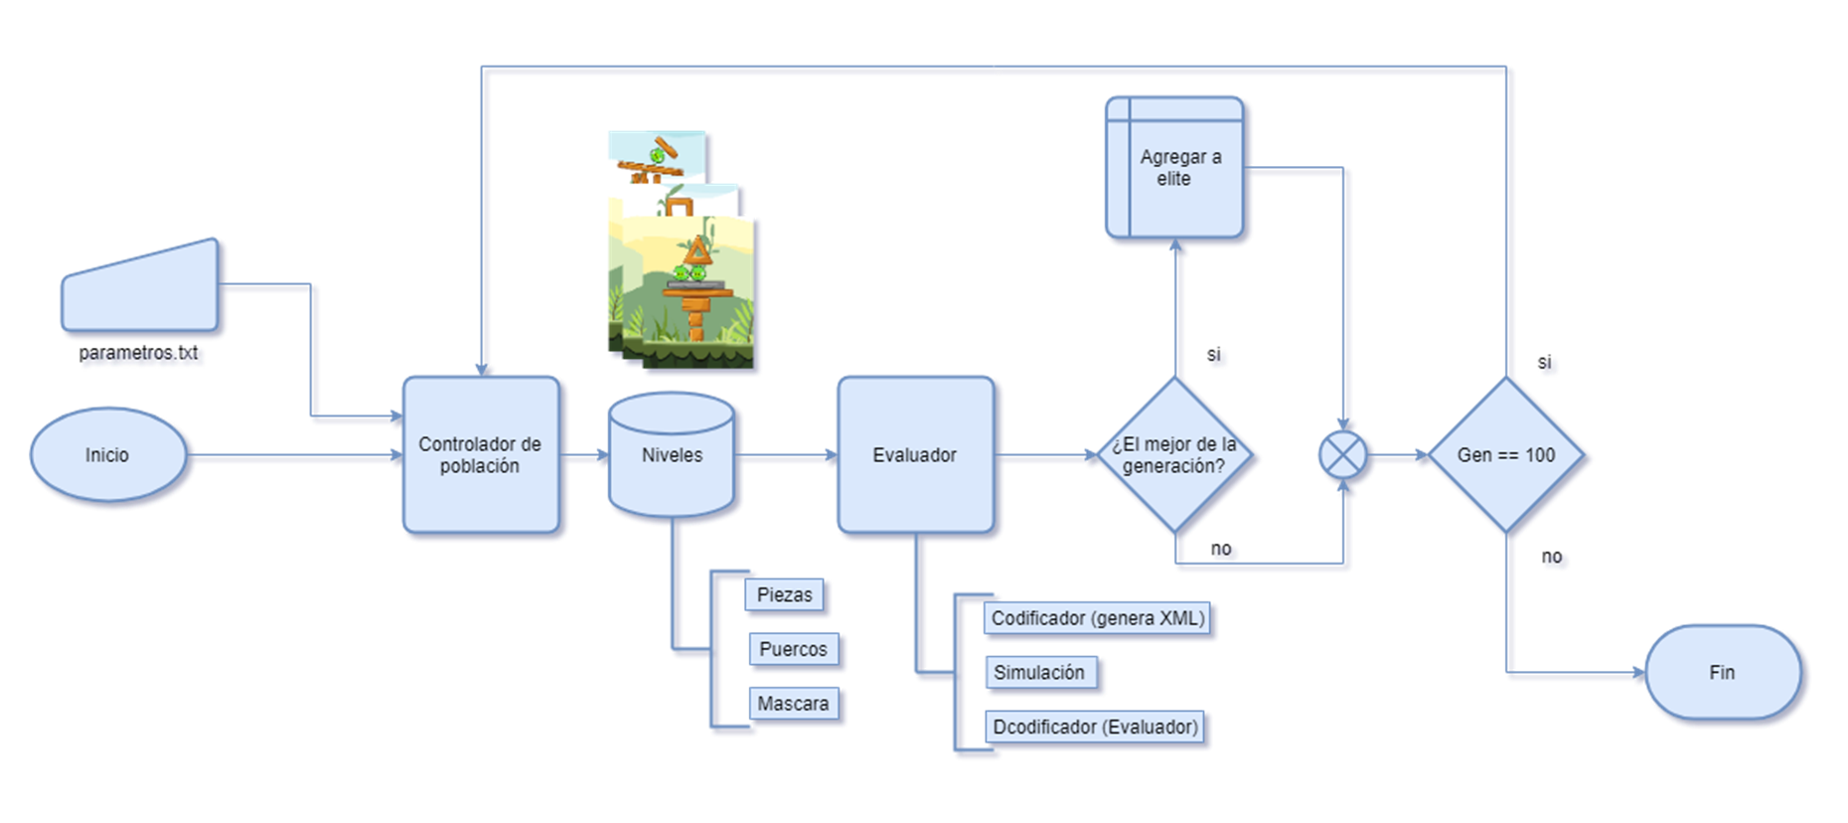
\includegraphics[width=1.0\textwidth]{img/system_model.png}
  \caption{Diagrama de flujo del algoritmo}
  \label{figure:algorithm_model}
\end{figure}

\section{Propuestas anteriores}
\label{section:previous-proposed-methods}

Dentro del aspecto de generar compuestos nuevos para ser utilizados, previamente
se propuso utilizar los resultados de un nivel cómo compuestos para las
siguientes generaciones, un ejemplo de esto se muestra en la Figura
\ref{figure:prev_composite_proposal_bef_aft} en donde una estructura generada
mediante el algoritmo genético se simula en el juego y después de varios
segundos el resultante del mismo podía ser utilizado cómo un compuesto para la
siguiente generación, este método proveería una manera de tener compuestos
verificados cómo viables, sin embargo, se optó por utilizar el generador de
compuestos antes de entrar al ciclo del algoritmo genético.

\begin{figure}
  \centering
  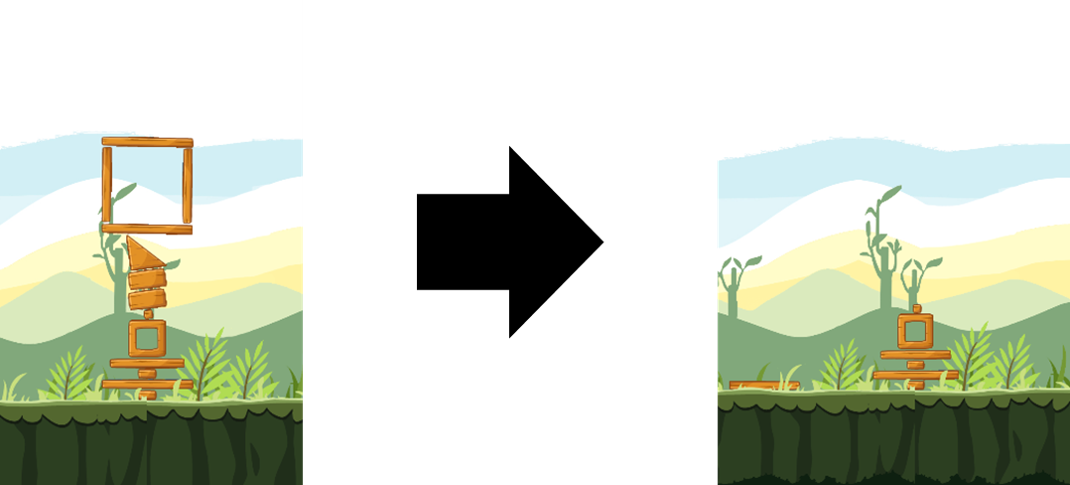
\includegraphics[width=1.0\textwidth]{img/simulation_bef_aft_example.png}
  \caption{Ejemplo de una estructura antes(izquierda) y después(derecha) de una simulación}
  \label{figure:prev_composite_proposal_bef_aft}
\end{figure}

\subsection{Propuesta orientada a métodos}
\label{subsection:objectorientedidea}

Una de las maneras en las que se propuso originalmente el desarrollo del proyecto
fue mediante el uso de diccionarios en Python, esto permitiría
tener un control de los compuestos generados debido a que mediante el uso de
diccionarios se podía generar un apuntados que permitiría que al momento de
generar los cromosomas de los individuos de la población estos utilizarán
simplemente listas numéricas que hicieran referencia al compuesto al cual
pertenecían, esto al final permitiría generar un solo diccionario que
contuviera todos los apuntadores a los compuestos generados.

Esto sin embargo presentó un problema para la generación de nuevos compuestos
debido a que en caso de querer realizar pruebas restringiendo el uso de ciertas
piezas o ciertas combinaciones de material-pieza se tenía que cambiar cada
elemento en el diccionario generado, además de esto se requería que las
piezas pudieran no solo restringirse, sino que se pudieran realizar cambios en
las maneras de cómo se generaban de manera sencilla, por tal se descartó esta
propuesta con el fin de utilizar la propuesta de generación de elementos
mediante el uso de clases cómo se explicó en el capítulo
\ref{subsection:classorientedidea}.

Además de esto otro de los problemas que se presentaban mediante el uso de
métodos para la generación de los cromosomas fue que los métodos se asignaban de
manera directa a los individuos lo cual provocaba que simplemente se asignaran
diccionarios que especifican el conjunto de métodos que se deberían de llamar,
sin embargo, al no tener los beneficios de un sistema de clases que puede ser
re-instanciado en caso de ser requerido se tiene el problema de que cada que se
realiza una modificación en los métodos, los cambios se propagan a los
demás individuos provocando errores en los niveles generados.


\subsection{Regla de tercios}
\label{subsection:ruleofthirds}

Uno de los temas que más interesaba en la generación de niveles fue la manera en
cómo se acomodarían las estructuras en al área del juego, debido a que lo que se
buscó en el proyecto originalmente fue crear estructuras que tuvieran una gran
altura y lograran mantenerse estables se buscaron maneras de lograr que el
posicionamiento de las piezas o compuestos fuese lo más \textit{'controlado'}
posible debido a que simplemente colocar piezas al azar generaría demasiada incongruencia
en los niveles generados, por tal motivo una de las primeras propuestas fue el
uso de la \textit{regla de tercios}.

La regla de tercios es una técnica utilizada en el área de fotografía cuyo
propósito es crear imágenes estéticamente agradables a la vista en donde el
punto focal o punto de interés se encuentra colocado en la alguna de las áreas
de la imagen, un ejemplo de esto se puede apreciar en la Figura
\ref{figure:ruleofthirdsexample} en donde el objeto principal que se quiere
resaltar se trata de colocar en el área central de la imagen completa.

La regla de tercios hace uso de líneas imaginarias que dividen la imagen en nueve
áreas, y mediante el uso de la
cuadricula generada se colocan los objetos principales de una imagen entre
líneas divisorias de tal manera que en caso de imágenes grandes donde existen dos
o más elementos importantes un solo objeto no tome el centro absoluto de la
imagen, sino que se mantenga alineado a un punto donde las líneas se cruzan para
que los demás elementos de la imagen tengan un mismo nivel de interés y en el
caso de que solo sea un elemento no utilice toda la parte central de la imagen
sino que exista un nivel de balance en la imagen en donde el cielo o el fondo
tenga una tercera parte del espacio de la fotografía, mientras que el área
activa o el área inmediatamente adyacente al sujeto de la imagen cubra el
resto de la misma.

La manera en cómo se planeó utilizar esta técnica es mediante el uso de una
cuadricula de tres por tres de la misma manera que se me muestra en la Figura
\ref{figure:ruleofthirdsexample}, pero en el caso de los niveles generados se
espera utilizar la cuadricula para rellenar áreas del nivel iniciando desde la
parte inferior para generar niveles más robustos en sentido de que la
distribución de las piezas es más enfocada al centro creando una pirámide o
llenando todas las áreas dependiendo de la cantidad de piezas utilizadas. 

\begin{figure}
  \centering
  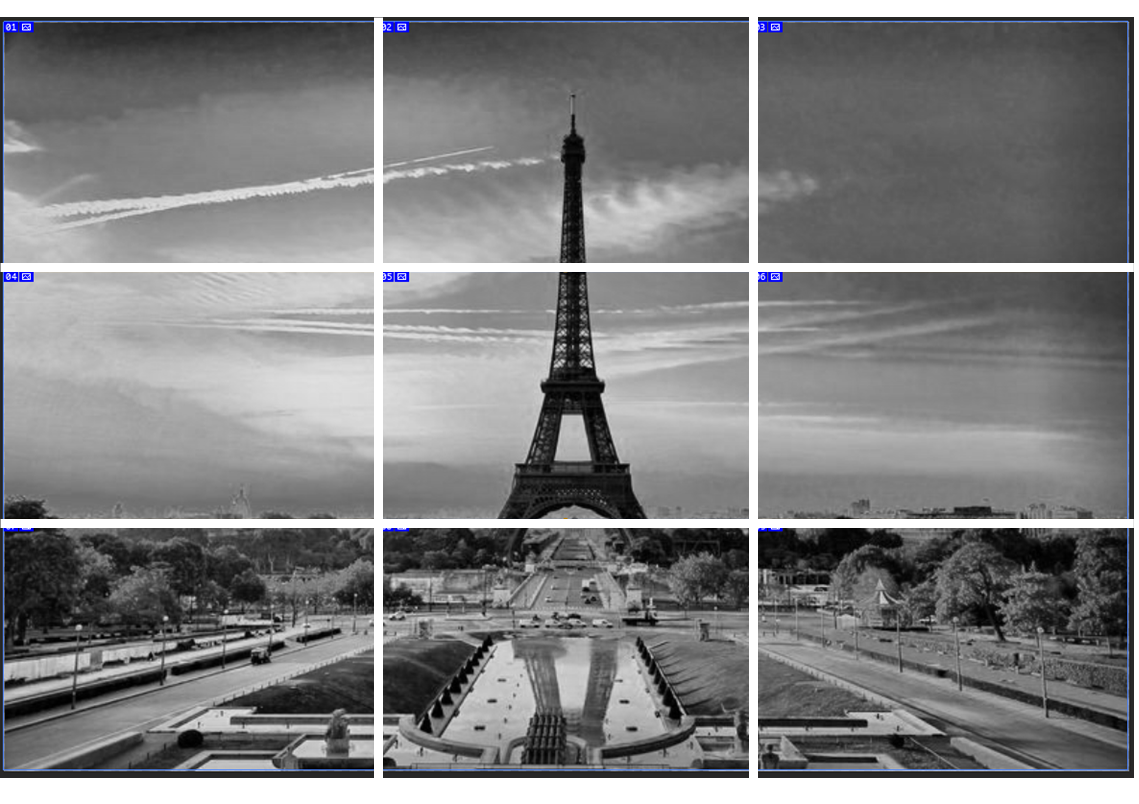
\includegraphics[width=1.0\textwidth]{img/ruleofthirds_example.png}
  \caption{Ejemplo del uso de la regla de tercios en una imagen, el punto de interés se encuentra en la parte central}
  \label{figure:ruleofthirdsexample}
\end{figure}

Debido a que los niveles generados tienen un área de visión o área jugable
variante hasta cierto punto, se definirá un área de juego estática para los
niveles de tal forma que todos siempre se generen con las mismas dimensiones, de
esta manera se evita el tener que estar calculando áreas para los nueve
cuadrantes utilizando la regla de tercios y se utilizan siempre los mismos
valores para distribuir las piezas en los niveles.

El uso de la regla de tercios dentro
del proyecto fue mediante la utilización de máscaras de generación, estas máscaras se
generaron mediante la modificación de la idea detrás de la regla de tercios,
esto se utilizó de igual manera una cuadricula que cubriera el área de juego, la
cuadricula se modificó para cubriera el área con un tamaño de 3 cuadros de
altura y 7 cuadros de largo, de esta manera las piezas tendrían un poco más de
libertad sobre el dónde sería posible colocarlas, el ejemplo básico de la idea
detrás del uso de la regla de tercios se muestra en la Figura
\ref{figure:ruleofthird_on_pieces} en donde se utiliza una máscara simple para
acomodar los elementos en un individuo de tal manera que el ordenamiento dentro
de la cuadricula permitiría la generación de estructuras más complejas, sin
embargo esta idea a pesar de proveer una buena mecánica en el acomodo de las
piezas conllevaba un error debido que no solo se debería de buscar los puntos en
los cuales los elementos se podrían apoyar entre ellos, si no que era requerido
tomar en cuenta las posiciones, alturas, tamaños y ángulos de todos los
elementos presentes en el cromosoma una vez colocados en el nivel, los
resultados obtenidos utilizando la regla de tercios se muestran en la Figura
\ref{figure:ruleofthird_on_chromosome}, en esta imagen se muestra cómo una
máscara pre-generada con una forma de castillo mostrada del lado izquierdo de la
imagen se combina con el cromosoma entrante de un individuo para generar el
nivel mostrado del lado derecho de la imagen, este nivel se trata de asemejar a
lo establecido en la máscara, mientras que el uso de máscaras pre-generadas
permite encaminar el sistema de generación a un conjunto de resultados de igual
manera inhibe que se logre tener una diversidad de niveles debido a que siempre
se mantendrán dentro de las formas especificadas por las máscaras, debido a esto
se optó por modificar la idea para permitir que los individuos tengan una
máscara no pre-generada, sino que de manera pseudoaleatoria se les asigna una
máscara que contendrá de igual manera varias columnas en donde el total de
piezas se reparte de manera aleatoria, esto permitirá tener más diversidad en
los niveles generados.

\begin{figure}
  \centering
  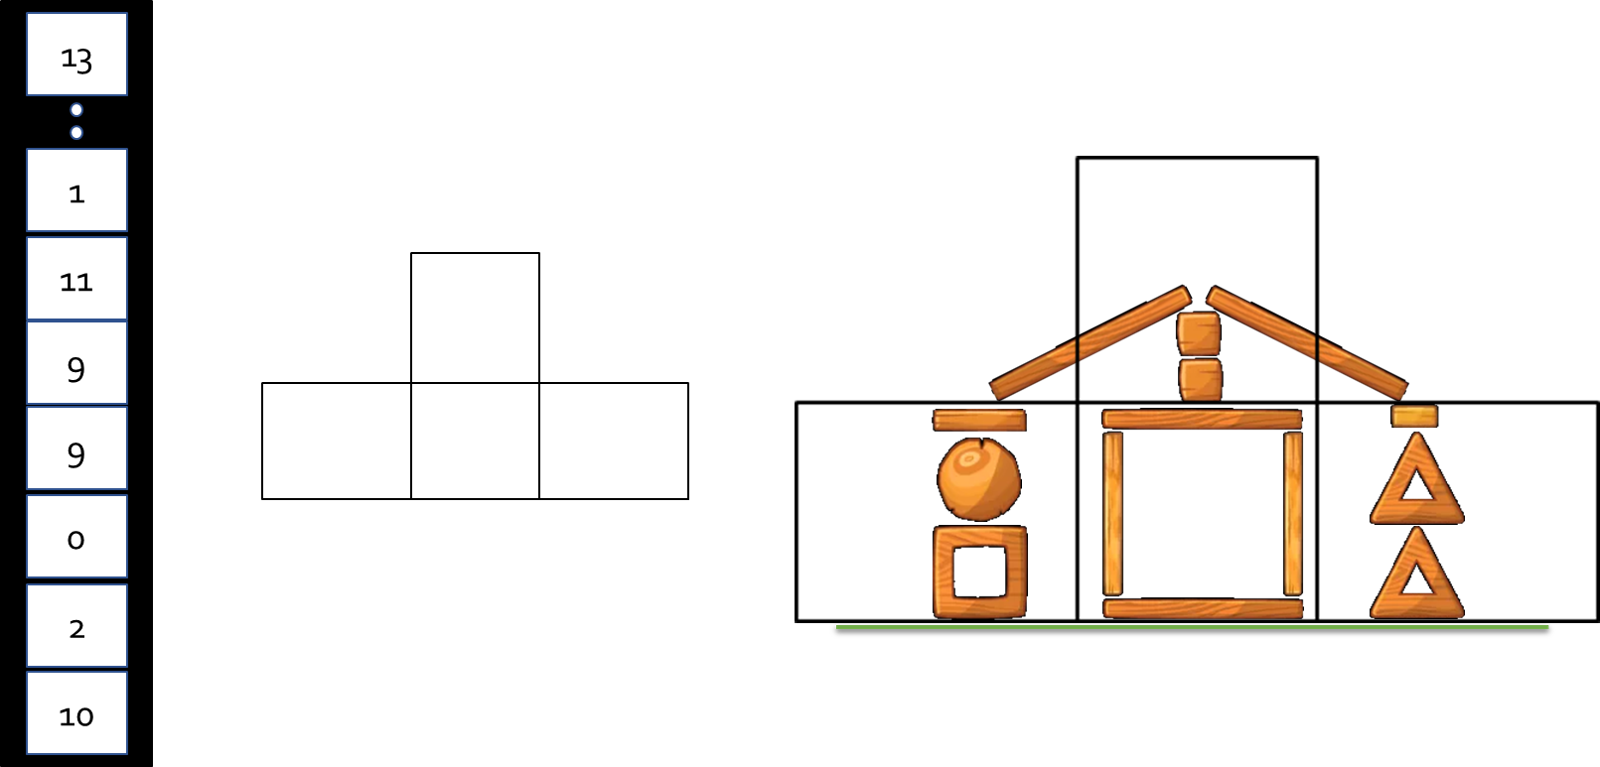
\includegraphics[width=1.0\textwidth]{img/chromosome_thirds.png}
  \caption{Ejemplo del uso de la regla de tercios en un conjunto de piezas, el cromosoma de un individuo(izquierda) se combina con la máscara(centro) para generar una estructura más compleja(derecha)}
  \label{figure:ruleofthird_on_pieces}
\end{figure}

\begin{figure}
  \centering
  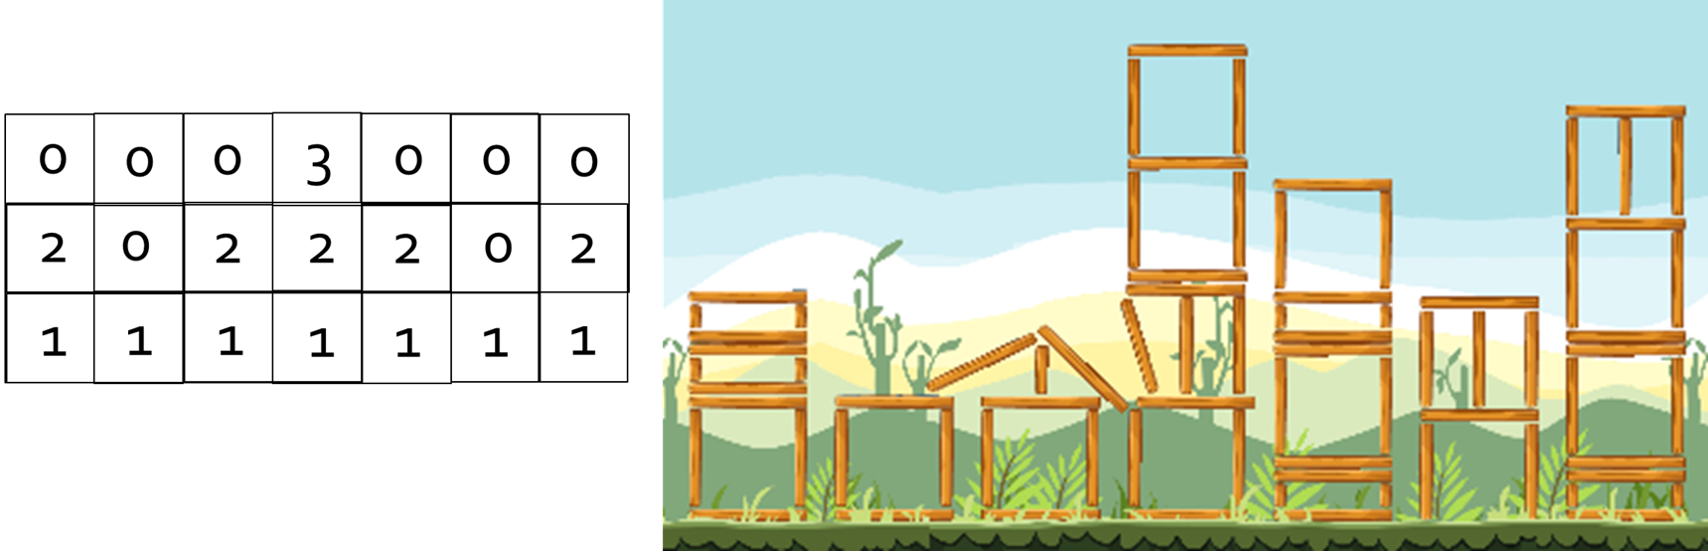
\includegraphics[width=1.0\textwidth]{img/result_example_thirds.png}
  \caption{Resultado obtenido utilizando la regla de tercios, la máscara(izquierda) utilizada y el resultado generado(derecha)}
  \label{figure:ruleofthird_on_chromosome}
\end{figure}



\chapter{Implementación}
\label{chapter:implementation}

El siguiente conjunto de secciones describen la implementación del método
propuesto según las explicaciones presentadas en el Capitulo
\ref{chapter:proposed-method}. La implementación propuesta utiliza un software
de simulación cómo el mostrado en \cite{Renz2013}
(\url{https://aibirds.org/other-events/level-generation-competition/basic-instructions.html}),
este software de simulación está programado en Unity con código fuente en
lenguaje C\# de Visual Studio.

\section{Codificando los diccionarios de piezas}
\label{section:piece_dictionary}

La primera parte que se desarrolló para poder integrar el listado de piezas al
sistema de generación fue decir la manera en cómo se establecerían las
diferentes piezas cómo las mostradas en la figura \ref{figure:game-basic-blocks}
del Capitulo \ref{chapter:proposed-method}, para esto se tomaron en cuenta
varias posibilidades, la primera, cómo se explica en la sección
\ref{subsection:objectorientedidea} se buscaba ordenar las diferentes piezas
cómo diccionarios que contuvieran una o más referencias a las piezas que
integraban cada entrada del diccionario, para esto las primeras 11 posiciones
eran elementos individuales uno para cada pieza cómo el mostrado en la figura
\ref{code:dic_individual_piece}, en el código se aprecia la manera en cómo se
designaba una pieza del juego, para poder trabajar de manera dinámica para poder
agregar más compuestos según fuese necesario se utilizaban dos diccionarios
extra, estos contenían los datos de los tipos de materiales posibles y la
información de los tamaños de las piezas, de esta manera en caso de tener más de
una pieza en algún punto del diccionario era posible modificar el valor de
offset de cada una de las piezas calculando la distancia del punto central de
cada pieza al centro de todo el conjunto.

\begin{listing}[t]
  \begin{minted}[frame=lines, framesep=2mm,baselinestretch=1.2,fontsize=\footnotesize,linenos]{python}
    BLOCKS = {
      0: [
          {'type': BLOCK_TYPE['Circle'],
          'material': BLOCK_MATERIAL['wood'],
          'offset': [0, 0, 0] # x, y, z - Calculated from the center of the figure
          }]
    }

    BLOCK_TYPE = {
    'Circle': {'height': 72, 'lenght': 72},
    'RectTiny': {'height': 22, 'lenght': 42},
    'RectSmall': {'height': 22, 'lenght': 42},
    'RectBig': {'height': 22, 'lenght': 42},
    'RectMedium': {'height': 22, 'lenght': 42},
    'RectFat': {'height': 42, 'lenght': 82},
    'SquareTiny': {'height': 22, 'lenght': 22},
    'SquareSmall': {'height': 42, 'lenght': 42},
    'Triangle': {'height': 72, 'lenght': 72},
    'TriangleHole': {'height': 82, 'lenght': 82},
    'SquareHole': {'height': 82, 'lenght': 82}
    }

    BLOCK_MATERIAL = {
        'wood': 0,
        'stone': 1,
        'ice': 2
    }
  \end{minted}
  \caption{Ejemplo de diccionario con un solo elemento}
  \label{code:dic_individual_piece}
\end{listing}

De esta manera cómo se explicó anteriormente era más sencillo crear compuestos,
sin embargo, la desventaja que conllevaba utilizar este método era que no podían
realizar modificaciones a las restricciones de las piezas, es decir, en caso de
querer evitar que un conjunto de piezas con determinados materiales no fueran
generados no se tenía la facilidad de impedir este tipo de combinaciones.

En luz de esta información se optó por utilizar el método en base a clases
mencionado en la sección \ref{subsection:classorientedidea}, el código
\ref{code:dic_individual_piece} muestra la nueva estructura utilizada según el
diagrama de clases presentado en la figura \ref{figure:pieces-class-diagram},
de acuerdo al diagrama presentado una clase base con las operaciones y
propiedades necesarias funcionaria cómo una clase \textit{padre} para las clases
de piezas particulares, de esta manera los individuos se representarán cómo un
conjunto de referencias a las clases que deben de ser generadas para la
composición de niveles, sin embargo, está manera de representar a los individuos
no contempla las restricciones que pueden ser definidas para la combinación de
piezas-materiales, debido a esto se optó por generar una lista global que
mantuviera un récord de las restricciones aplicadas en el sistema, y al momento
de generar cada re-instanciacion de clase para los individuos está información se
pasará a las clases según fuese requerido, en el código se presenta una variable
con el nombre \textit{mat}, está variable tomara una lista de 3 valores que
define si alguno o algunos de los materiales no puede ser utilizado al momento
de asignar las clases a los individuos, al momento de encontrar una pieza que de
la coincidencia no puede ser utilizada con ningún material se eliminarán los
datos de la pieza generada y se pedirá al sistema genere otra de manera aleatoria.

\begin{listing}[ht]
  \begin{minted}[frame=lines,framesep=2mm,baselinestretch=1.2,fontsize=\footnotesize,linenos]{python}
    class Circle(Piece):
      def __init__(self, mat, x=0, y=0, r=0):
          self.Name = "Circle"
          self.Height = 75
          self.Width = 75
          Piece.__init__(self, x, y, r, mat)
          self.update_values()
  \end{minted}
  \caption{Ejemplo de estructura de las clases hija que heredan de la principal}
  \label{code:dic_individual_piece}
\end{listing}

\section{Creación de compuestos}
\label{section:composite_creation}

Una vez definidas las clases particulares que controlaran la información de las
piezas en el algoritmo se procede a definir la manera en cómo se entregarán y
controlaran los diferentes compuestos de piezas, para términos más simples los
compuestos son grupos de una o más piezas y se mostraran a manera de diccionario
de listas cómo se muestra en el código \ref{code:dic_composites}, de esta manera
cada entrada en el diccionario tiene por nombre o apuntador el valor posición
según se fueron agregando al diccionario mientras que el contenido es una lista
con tuplas donde se estipula la información pertinente de cada pieza en el
compuesto, un ejemplo claro es el elemento en la posición \textit{9} el cual
cuenta con 3 piezas que muestran los valores de offset medida desde el centro
del compuesto visto gráficamente en el juego, está lista se utiliza para
mantener un control de los compuestos que se pueden ir agregando durante la
ejecución del algoritmo, de tal manera que las clases auxiliares de
\textit{Composite} creadas harán referencia a una o más piezas según la lista se
haya proporcionado al crear el compuesto.

\begin{listing}[ht]
  \begin{minted}[frame=lines,framesep=2mm,baselinestretch=1.2,fontsize=\footnotesize,linenos]{python}
    Composites = {
      0: [("RectTiny", 0, 0, 0, "wood")],
      1: [("RectSmall", 0, 0, 0, "wood")],
      2: [("RectMedium", 0, 0, 0, "wood")],
      3: [("RectBig", 0, 0, 0, "wood")],
      4: [("RectFat", 0, 0, 0, "wood")],
      5: [("SquareSmall", 0, 0, 0, "wood")],
      6: [("SquareHole", 0, 0, 0, "wood")],
      7: [("Circle", 0, 0, 0, "wood")],
      8: [("TriangleHole", 0, 0, 0, "wood")],
      9: [("RectBig", 100, 5, -27, "wood"), ("RectBig", -100, 5, 27, "wood"), ...
            ...("RectSmall", 0, 0, 90, "wood")]
    } 
  \end{minted}
  \caption{Diccionario con los compuestos existentes}
  \label{code:dic_composites}
\end{listing}

\section{Definición de clase auxiliar de individuo}
\label{section:definition_of_clases}

Mediante el uso de la clase de composite se tiene un mejor control de los genes
que conformaran cada individuo de la población, una vez que se tiene este
aspecto controlado el siguiente paso es el de crear programar la clase que
llevará el control de los cromosomas de un individuo, siendo los cromosomas los
compuestos asignados a cada individuo particular, de tal manera que un individuo
dentro de la información de cromosomas hará referencia a otra lista de
compuestos, la manera en cómo un \textit{Individuo} relaciona los compuestos es
mediante el uso de la línea de código:

\begin{minted}{python}
  chromosome_objects = [Composite(Composites[composite]) for composite in self.chromosome]
\end{minted}

Mediante esta línea de código se indica que se deberá de crear una lista en donde
cada elemento será una instancia de un compuesto asignado al individuo, de está
manera si se requiere modificar la posición o materiales de un compuesto
particular en el individuo es posible hacerlo desde la clase de
\textit{individuo}, de igual manera está clase tiene cómo funciones principales
cómo se muestran en el diagrama de clase de la figura
\ref{figure:individual-class-diagram} realizar los cálculos de fitness y generar
las listas de piezas que serán utilizadas para generar los archivos de salida
necesarios para las simulaciones de los niveles generados.

\section{Generación de individuos}
\label{section:ind_generation}

Una vez definida la manera de controlar las clases el paso siguiente es el de
comenzar con la generación de ls individuos de la población, para poder lograr
esto se creó una línea de código en la cual los puntos necesarios para la
generación de los individuos se entregan totalmente, está línea de código en
cuestión es cómo sigue: 

\begin{minted}{python}
  pop = [Individual(chromosome = get_random_chrom(ind_pieces), ..
    ..másk = create_new_másk(ind_pieces)) for i in range(population)]
\end{minted}

Mediante el uso de esta línea de código se le indica al sistema que se requiere
una lista que representara a los individuos de la población, cada elemento de
está lista será una instancia independiente de la clase \textit{Individual},
para generar está instancia de clase es requerido dos valores siendo estos
primero una lista de valores numéricos que representan cuales piezas se
asignaran a los individuos, para generar está lista se utiliza una función cómo
se muestra en el código \ref{code:get_random_chrom}, el segundo dato requerido
es una segunda lista que denota una máscara mediante la cual las piezas
asignadas serán acomodadas al momento de generar los archivos de simulación,
finalmente, la última sección del código - \textit{for i in range(population)} -
denota que el proceso se deberá de repetir una cierta cantidad de veces, es
decir que pada cada individuo se generara una instancia con valores diferentes a
los anteriores, la cantidad de vences que se deberá de repetir depende de la
cantidad de individuos con los que se quiere estar trabajando en el algoritmo en
el caso de las pruebas realizadas se utilizó un total de 10 individuos lo que
significa que la lista \textit{pop} generada consta de 10 instancias diferentes
de la clase \textit{Individual}. 

Para la generación de la lista de piezas o cromosomas asignados a un individuo
mostrada en la parte (1) del código en \ref{code:get_random_chrom}, aquí el
valor que se recibe denota la cantidad de piezas o compuestos que se deberán de
asignar en la lista para el individuo, para asignar estos valores primero se
obtiene un numero aleatorio que va desde \textit{0} hasta la cantidad de piezas o
compuestos presentes en la lista menos una unidad para evitar errores de
posicionamiento de lista, posteriormente se revisa si la pieza seleccionada
puede ser utilizada al menos en una combinación dentro de la generación, en caso
de que no puede ser utilizada se obtiene otra y de igual manera se revisa, en
caso de poder ser utilizada se agrega a la lista y avanza un contador para saber
cuando se llegue al límite de piezas posibles de usar, finalmente se entrega la
lista de piezas para la generación de la instancia de clase. Para la generación
de la máscara de acomodo de piezas se utiliza la sección de código mostrado en
la parte (2), en esta parte lo que se realiza es que se revisa la cantidad de
compuestos que se pueden utilizar cómo en la parte anterior, este valor se
utiliza posteriormente para generar una lista aleatoria, la lista que se genera
tiene un total de 7 posiciones que denotan 7 divisiones que se realizan en el
área de un nivel para el acomodo de las piezas, mediante el uso del valor de
piezas en cada individuo se realiza una aleatorización de números desde
\textit{0} hasta la cantidad máxima de piezas, una vez se obtienen estos valores
aleatorios se revisa si la suma de estos da la cantidad de piezas en el
individuo, en caso de que no sea así se repite el proceso, en caso de que si se
cumpla entonces la lista se regresa para la creación de la instancia de clase.

\begin{listing}[ht]
  \begin{minted}[frame=lines, framesep=2mm, baselinestretch=1.2, fontsize=\footnotesize, linenos]{python}
 (1)  def get_random_chrom(sl):
        asl = 0
        chrom = []
        while asl < sl:
            prop = random.randint(0, len(Composites)-1)
            if clases[Composites[prop][0][0]].Valid == True:
                chrom.append(prop)
                asl += 1
        #random.randint(0,len(Composites)-1) for p in range(ind_pieces)
        return chrom

 (2)  def create_new_másk(pieces):
        div_list =[]
        while True:
            div_list = [random.randint(0, pieces-1) for col in range(7)]
            if sum(div_list) == pieces:
                break
          
        return div_list
  \end{minted}
  \caption{Código de asignación de cromosomas(piezas)[1] y código para generar máscaras [2]}
  \label{code:get_random_chrom}
\end{listing}

Una vez que se ha logrado crear la lista de individuos se procede a inicializar
el algoritmo evolutivo, este algoritmo se ejecutará una determinada cantidad de
veces que se haya establecido en el código, el pseudo-código ah ejecutar con su
respectiva implementación en código se enlista a continuación en el código
\ref{code:algorithm_pseudocode}, este pseudocódigo engloba los aspectos
principales del sistema de generación de niveles, el código se explica más a
detalle en las secciones siguientes.

\begin{listing}[ht]
  \scalebox{.8}{\noindent%
\begin{Heardlisting}{%
   \begin{tabular}{r}% 
      Integrar miembros "elite" (1-4)\\ \\  \\  \\  \\
      Simular individuos (6)\\  \\
      Calcular fitness (8-9)\\  \\  \\
      Obtener padres de la generacion (10)\\  \\
      Realizar crossover (12)\\ \\
      Seleccionar elite (14-15)\\ \\
   \end{tabular}
}
if elite not null
   for member in elite
      population <- member
      trim population

execute process (game)

for individual in population
   individual.getfitness

parents <- selector_operator(population, required)

crossover_operation(population, parents)

population.order('fitness')
elite.add(population[1])
\end{Heardlisting}}
  \caption{Pseudo-código del algoritmo genético}
  \label{code:algorithm_pseudocode}
\end{listing}

\subsection{Integración de miembros elite}
\label{subsection:elite_member_integration}

Está parte se encarga de iniciar los bucles de generación, la función principal
de este bloque de código es la revisar la lista auxiliar de miembros de elite
que existe en memoria, en caso de tener elementos en la lista estos se integran
a la lista de la población integrándose al inicio de la misma, una vez agregados
todos los miembros la lista de la población se corta hasta el numero máximo de
miembros permitidos en las generaciones, este valor se asigna cómo un valor de
entrada al inicio del archivo que contiene el código.

Una vez terminada está acción se procede a denotar la cantidad de padres que
serán necesarios para generar los hijos de las generaciones futuras, esto se
hace mediante el cálculo:
\begin{minted}{python}
  many = len(pop) * per_cross
\end{minted}
En donde \textit{pop} representa la lista de miembros de la población,
\textit{per\_cross} representa un valor entre \textit{0\.0} y \textit{1\.0}, este
valor representa que tanto porcentaje de la población se quiere realice cruces,
de está manera la variable \textit{many} representa la cantidad de individuos
que se deberan de utilizar para cumplir el porcentaje de cruce, debido a que el
valor de \textit{per\_cross} puede generar un valor flotante se tiene una parte
de código en donde si el total de individuos que realizaran cruces es un numero
impar entonces el valor que se deberá de utilizar será el numero par redondeado
hacia abajo, es decir, si de 10 individuos en la población se quiere que un
total de individuos cercano al \textit{50\%} realicen un cruce entonces el valor
resultante para la variable \textit{many} seria de 5, en este caso lo que se
hace es restar 1 al resultado y después se redondea hacia abajo, lo cual haría
que el número de padres requeridos para los cruces sea de 4.

Una vez que se tiene el valor de los padres requeridos para los cruces de la
generación se procede a crear los archivos auxiliares de los individuos de la
población, los archivos generados son en formato \textit{XML}, la información
que contienen estos archivos es la posición, tipo y material de ls piezas que
serán utilizadas en el nivel, además de esto también contiene la información de
la cantidad y tipo de aves así cómo de los enemigos que serán colocados, estos
archivos son almacenados en un folder en donde el software de simulación se
encarga de obtenerlos y entregar los resultados después de la simulación.

Una vez que los archivos de simulación han sido generados el algoritmo manda un
comando que manda la ejecución del software de simulación, el software en
particular cuenta con una ventana grafica en la que se puede apreciar los niveles
que se generaron o involucionaron en caso de estar simulando archivos de una
generación después de la primera, de igual manera el software genera un archivo
en formato \textit{XML} similar al que se genera antes de la simulación, la
diferencia entre ambos archivos es que el que es entregado después de la
simulación entrega los datos de posición del ultimo estado registrado del nivel,
además de que se puede solicitar que entregue el valor de la aceleración de la
misma, el valor de aceleración es tomado en cuenta desde el punto en el que la
pieza comienza su descenso, en caso de que una pieza sea destruida durante el
proceso de simulación ninguno de los datos de esa pieza son grabados en los
archivos, la manera de llevar control de las piezas que entran y las que salen
es mediante el uso de un numero de lista asignado al momento de generar los
archivos de simulación de la sección anterior.

Posterior a la simulación los archivos entregados son revisados y en base la
información de las piezas se calcula el \textit{Fitness} de las mismas,
posteriormente a esto se procede a ordenar la lista, y realizar las operaciones
de selección, cruce, mutación los cuales se explican en la sección siguiente.

\subsection{Operador de selección}
\label{subsection:sel_operator}

El proceso de selección se definió de dos maneras diferentes, la primer es
mediante el uso de una ruleta para las selecciones, en está ruleta los valores que
se toman en cuenta es el fitness de cada individuo, mientras más alto sea el
fitness mayor será la probabilidad de ser seleccionado para el cruce en la
siguiente sección.

El segundo método utilizado es la selección mediante torneo, en este tipo de
selección lo que se realiza es que los individuos se seleccionan en pares de
manera aleatoria, entre cada par se realiza un cálculo de cual tiene el mejor
fitness y ese individuo es seleccionado cómo padre para la generación.

\subsection{Operador de cruce}
\label{subsection:crossover_operator}

Para los operadores de cruce se tienen codificados dos tipos, cruce de un punto
y cruce de dos puntos, este operador de cruce se realiza no solo en los
individuos de la población sino también en las máscaras que tienen los mismos
individuos, esto es para aumentar un grado más el nivel de diversidad que se
puede tener en los individuos generados, la idea en este caso es lograr que
existan casos en donde la máscara sea muy chica y varias piezas de los
individuos no sean mostradas y el caso contrario permitirá que un individuo
pueda o no quedar con el mismo caso y puede que se dé el caso en donde alguno de
ambos elementos logren obtener un mejor nivel de fitness en la generación.

Un ejemplo de estos dos tipos de cruce se puede apreciar en la figura
\ref{figure:crossover} en donde dos individuos realizan un cruce con sus
máscaras y las máscaras generadas para los hijos resultan con diferente cantidad
de piezas.

La manera en cómo se aplican estos tipos de operador es:
\begin{enumerate}
  \item Definir un punto de corte igual para los dos individuos en cualquier
  posición de la lista de genotipos.
  \item Separar las dos partes cortadas de ambos individuos de tal manera que se
  tenga la parte de inicio (del inicio hasta el corte) y la parte final (desde
  el corte hasta el final) de cada individuo.
  \item Para crear al primer hijo tomar la parte inicial del primer individuo y
  unirla con la parte final del segundo individuo
  \item Para el segundo hijo tomar la parte inicial del segundo individuo y
  unirla con la parte final del primer individuo.
\end{enumerate}
De está manera los hijos se pueden comprender de la siguiente manera:
\begin{minted}{python}
  padre1 = padre[1, punto_corte]
  padre2 = padre[punto_corte, fin]

  madre1 = madre[1, punto_corte]
  madre2 = madre[punto_corte, fin]

  hijo1 = padre1 + madre2
  hijo2 = madre1 + padre2
\end{minted}
Para el caso del cruce de dos puntos la manera en cómo se realiza es que en vez
de dividir el genotipo de un individuo en dos partes se divide en tres y al
momento de realizar la combinación se toma la primer parte del primer individuo,
después la parte de enmedio del segundo individuo y finalmente la parte final
del primero, de tal forma que solo la parte central de ambos individuos se
cambia.

\begin{figure}
  \centering
  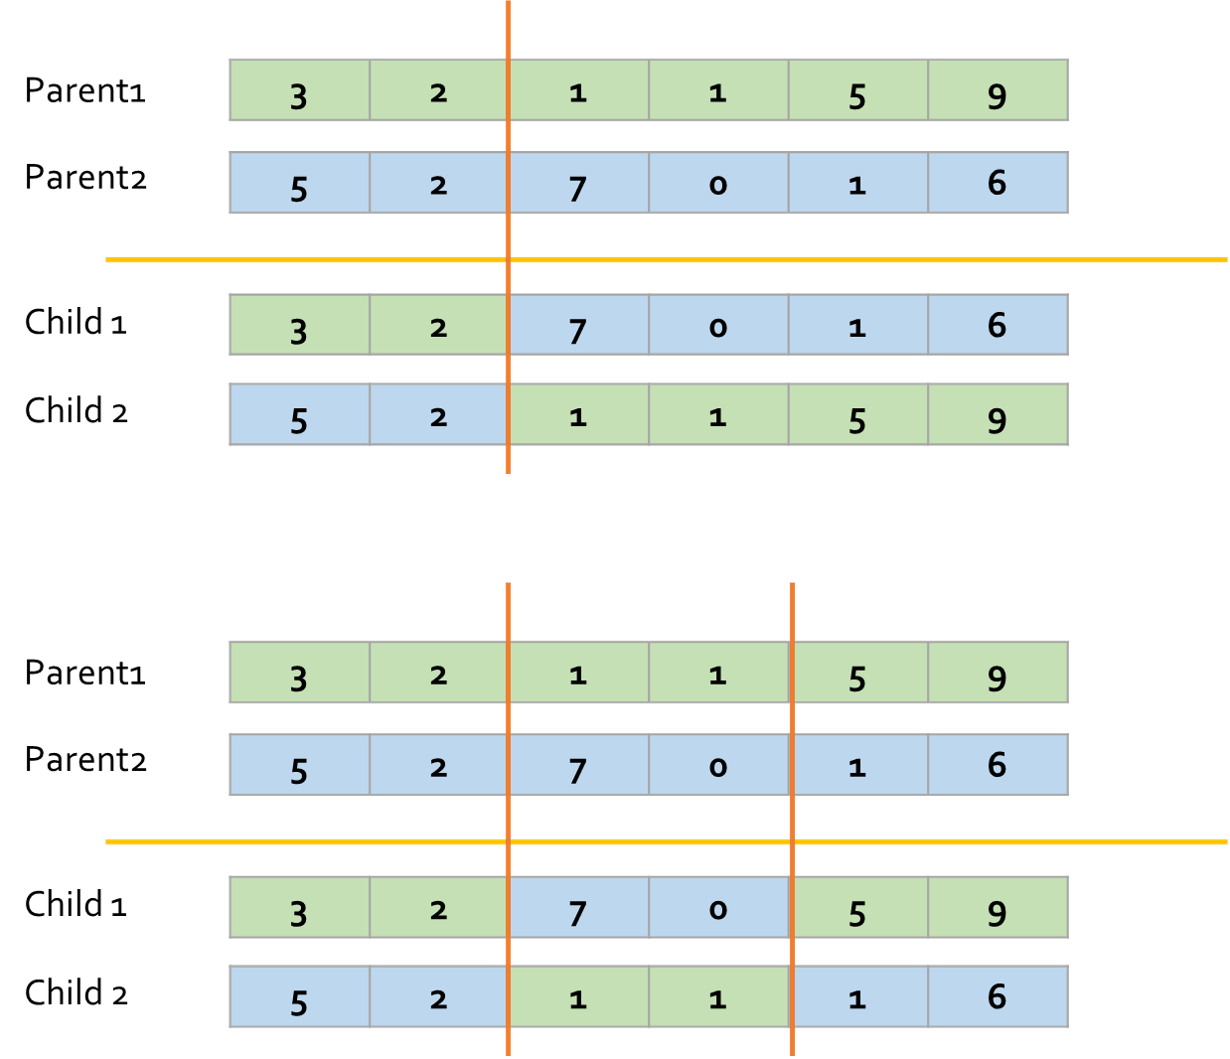
\includegraphics[width=0.8\textwidth]{img/crossover.png}
  \caption{Cruce de un punto (arriba) y cruce a dos puntos (abajo) aplicada a la máscara de individuos}
  \label{figure:crossover}
\end{figure}

\subsection{Operador de mutación}
\label{subsection:mutation_operator}

La mutación de los individuos de la población ocurre solo al momento de hacer el
cruce de los mismos, es decir solo a los elementos nuevos se les aplica el
operador de mutación, este operador puede modificar los siguientes elementos de
un individuo:
\begin{enumerate}
  \item La cantidad de piezas que conforman al individuo.
  \item El material del cual están formados los elementos.
  \item El tipo de elemento que conforma a un individuo, es decir, modificar el
  valor del compuesto que forma parte del individuo.
  \item La posición individual (\textit{x} o \textit{y}) de los compuestos.
\end{enumerate}

La manera en cómo se aplica el operador de mutación se describe cómo sigue,
primero al momento de generar al nuevo individuo se realiza un cálculo de
porcentaje en donde se decide si tendrá o no mutación dependiendo del porcentaje
de mutación que se haya asignado al inicio del algoritmo, posteriormente en caso
de que el valor de porcentaje quede dentro del rango se toma para las
operaciones, está mismas se explican de la manera siguiente.

Para mutar la cantidad de compuestos en un individuo primero se realiza una
selección aleatoria entre las opciones de agregar o quitar compuestos,
posteriormente en caso de requerir agregar más se realiza una selección
aleatoria de entre la cantidad de compuestos creados, estos mismos se integran
al final de la lista de compuestos del individuo. Para eliminar elementos de la
lista se realiza una corrida por todos los elementos y en cada uno se realiza
una probabilidad de \textit{50\%} de sea borrado de la lista, un ejemplo de este
proceso se muestra en la figura \ref{figure:mutate_add_remove} en donde se
presenta una tabla que denota las posiciones de los compuestos en base a la
máscara, en este ejemplo se realizó una corrida para remover elementos (color
rojo) y una segunda para agregar nuevos compuestos (color verde).

\begin{figure}
  \centering
  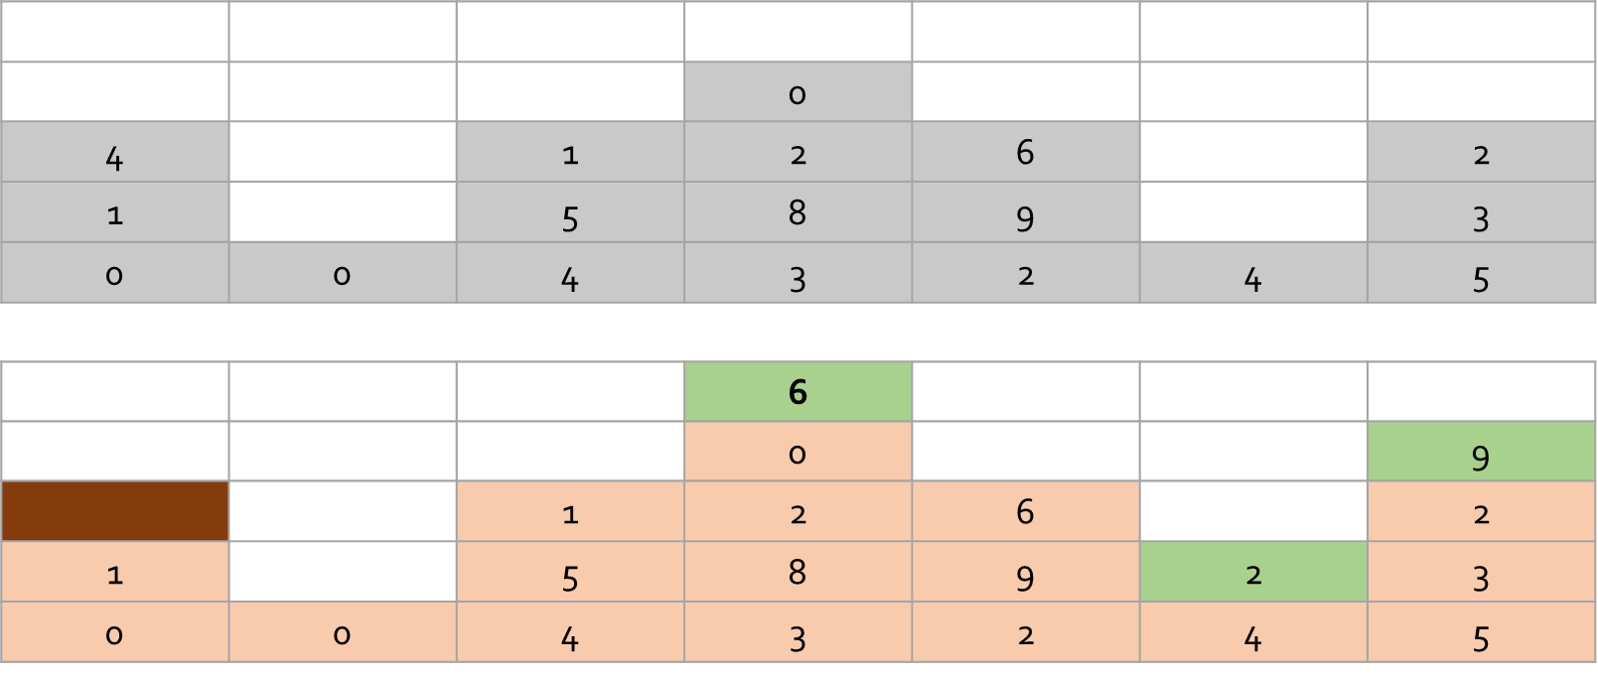
\includegraphics[width=0.85\textwidth]{img/mutation_add_remove.png}
  \caption{Ejemplo del operador de mutación enfocado a remover y agregar compuestos}
  \label{figure:mutate_add_remove}
\end{figure}

La segunda mutación se encarga de modificar el material del que están
conformados los compuestos del individuo, la manera en cómo trabaja este proceso
es primero se selecciona aleatoriamente cuales compuestos serán modificados sin
repetir valores, posteriormente se modifica de manera aleatoria el valor que
define el tipo de material del que se conforma, para esto se toma en cuenta que
\textit{0} representa material de madera, \textit{1} representa material de
hielo y finalmente \textit{2} representa el material de piedra, debido a que el
juego solo acepta está lista de compuestos no es posible asignar valores
diferentes a estos.

En la figura \ref{figure:mutate_material} se muestra un ejemplo de la manera en
cómo opera la mutación del tipo de compuesto, en este ejemplo se muestra el
genotipo y fenotipo de un individuo, el genotipo muestra los colores naranja,
azul y gris para denotar los materiales de madera, hielo y piedra
respectivamente, en este caso la mutación cambia el material de 5 elementos del
genotipo de madera a hielo, esto se refleja del lado derecho en donde se muestra
la vista actualizada del individuo después de la mutación.

Debido a que los compuestos generados pueden contener diferentes cantidades de
elementos en estos casos se cambia el material equitativamente a todos elementos
del compuesto, de esta manera se evita tener que realizar un recorrido por todo
el compuesto y mutar el material de cada uno.

\begin{figure}
  \centering
  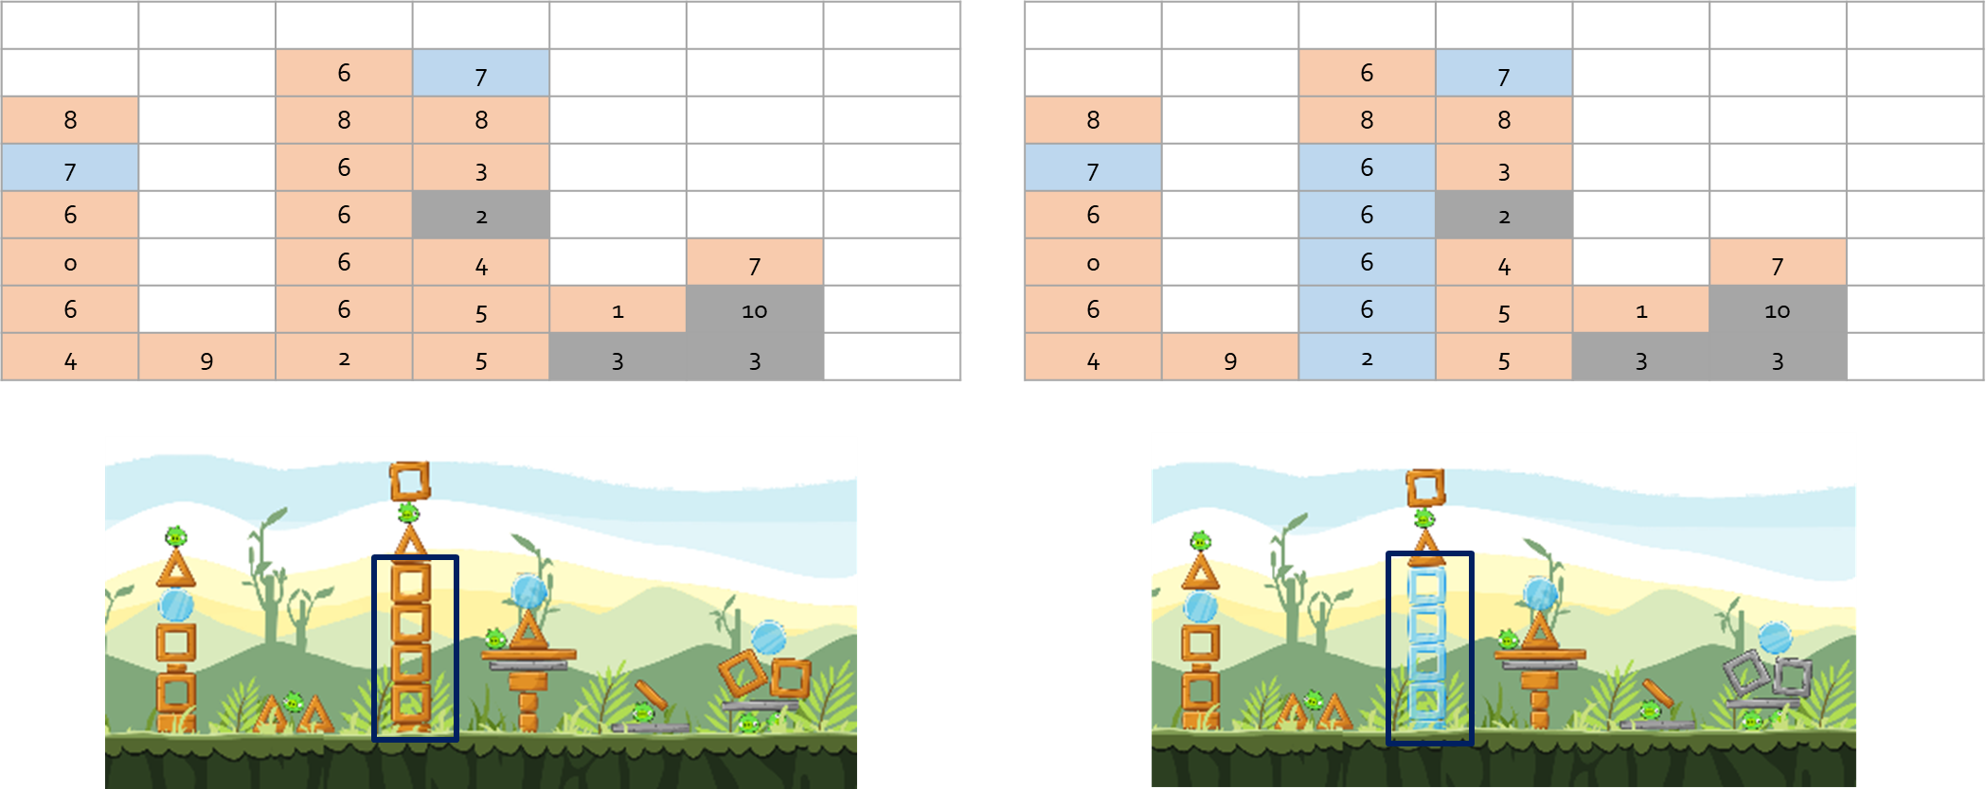
\includegraphics[width=0.95\textwidth]{img/mutation_material.png}
  \caption{Ejemplo del operador de mutación enfocado a cambiar el material de los compuestos, pre-mutación (izquierda) y post-mutación (derecha)}
  \label{figure:mutate_material}
\end{figure}

La tercera mutación se encarga de cambiar el compuesto que representa una
posición del genotipo del individuo, este trabaja de una manera similar al
anterior en el sentido de que primero se selecciona a los individuos a mutar,
posteriormente a la selección se realiza una segunda selección aleatoria entre
las posiciones del genotipo del individuo, aquellos compuestos seleccionados son
cambiados por otro de la lista existente, para esto se realiza una selección de
un valor aleatorio que va desde \textit{0} hasta la cantidad de compuestos
existentes, por ejemplo, suponiendo que se tiene solo la cantidad base de piezas
en el algoritmo entonces la selección será un valor aleatorio desde \textit{0}
hasta \textit{10}.

La figura \ref{figure:mutate_composite} nos muestra un ejemplo de cómo es que
actúa la mutación de tipo de compuesto, en el ejemplo mostrado se tiene el
genotipo de un individuo combinado con su respectiva máscara así cómo su
fenotipo respectivo (lado izquierda) al ser representado en la pantalla del
juego, en el lado derecho de la misma imagen se aprecia la modificación de
compuestos realizada al genotipo base (marcado en amarillo), la modificación de
compuestos en los individuos puede traer la consecuencia de que los niveles
generados sean inestables cómo en este ejemplo, esto a su vez puede permitir
identificar máscaras de los individuos que logran mantener la estabilidad de las
estructuras permitiendo así mejorar el algoritmo.

\begin{figure}
  \centering
  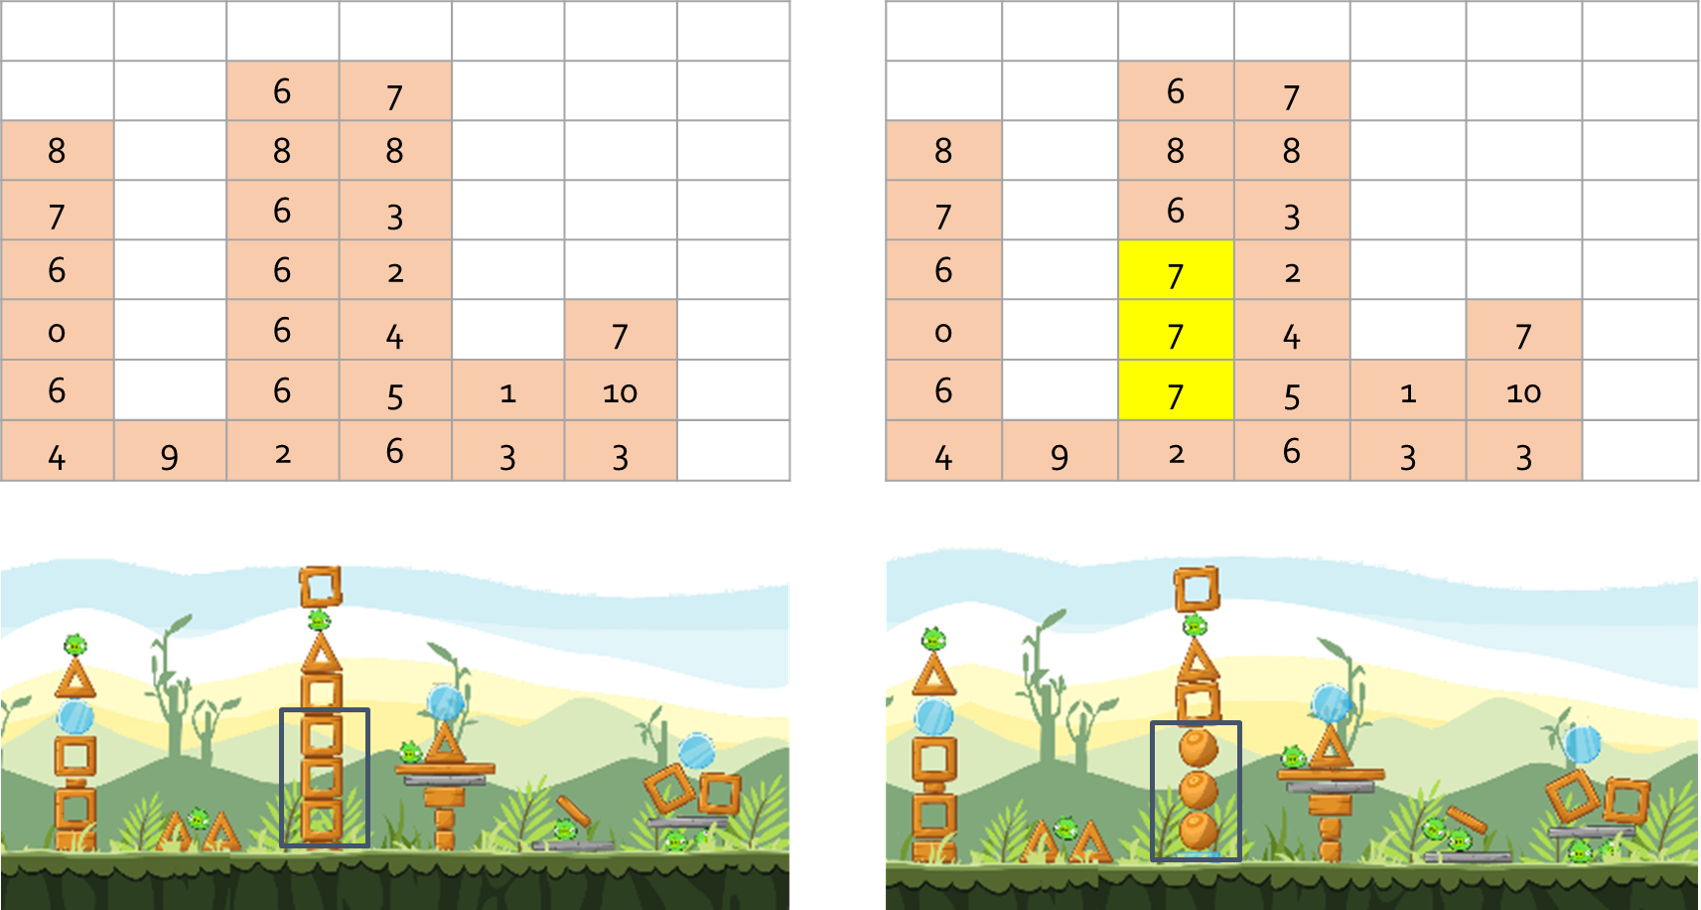
\includegraphics[width=0.9\textwidth]{img/mutation_composite.png}
  \caption{Ejemplo del operador de mutación enfocado a cambiar los compuestos asignados, pre-mutación (izquierda) y post-mutación (derecha)}
  \label{figure:mutate_composite}
\end{figure}

El ultimo tipo de mutación realizada en los individuos es la modificación de las
posiciones \textit{x} y \textit{y} de algunos compuestos dentro del individuo,
la modificación de las posiciones se realiza mediante una selección de valores
aleatorios de una distribución gaussiana dentro de un cierto rango de distancia
para no permitir que los elementos se alejen demasiado de punto central
original.

\subsection{Representacion de individuos}
\label{section:individual_representation}

Una vez que se han agregado nuevos individuos a la población, y que estos
individuos pasaron por su fase de mutación si es que requerían se procede a
realizar la combinación de los elementos que conforman al individuo con el fin
de generar los archivos requeridos para la simulación de estos mismos, cabe
resaltar que está combinación se realiza también en los individuos iniciales
antes de la simulación inicial, debido a que el juego requiere una
representación mediante el uso de archivos en formatos \textit{XML}, se requiere
primero obtener la información de todos los elementos que conforman a un
individuo y posteriormente armar los archivos mediante el uso de estos datos.

\begin{figure}
  \centering
  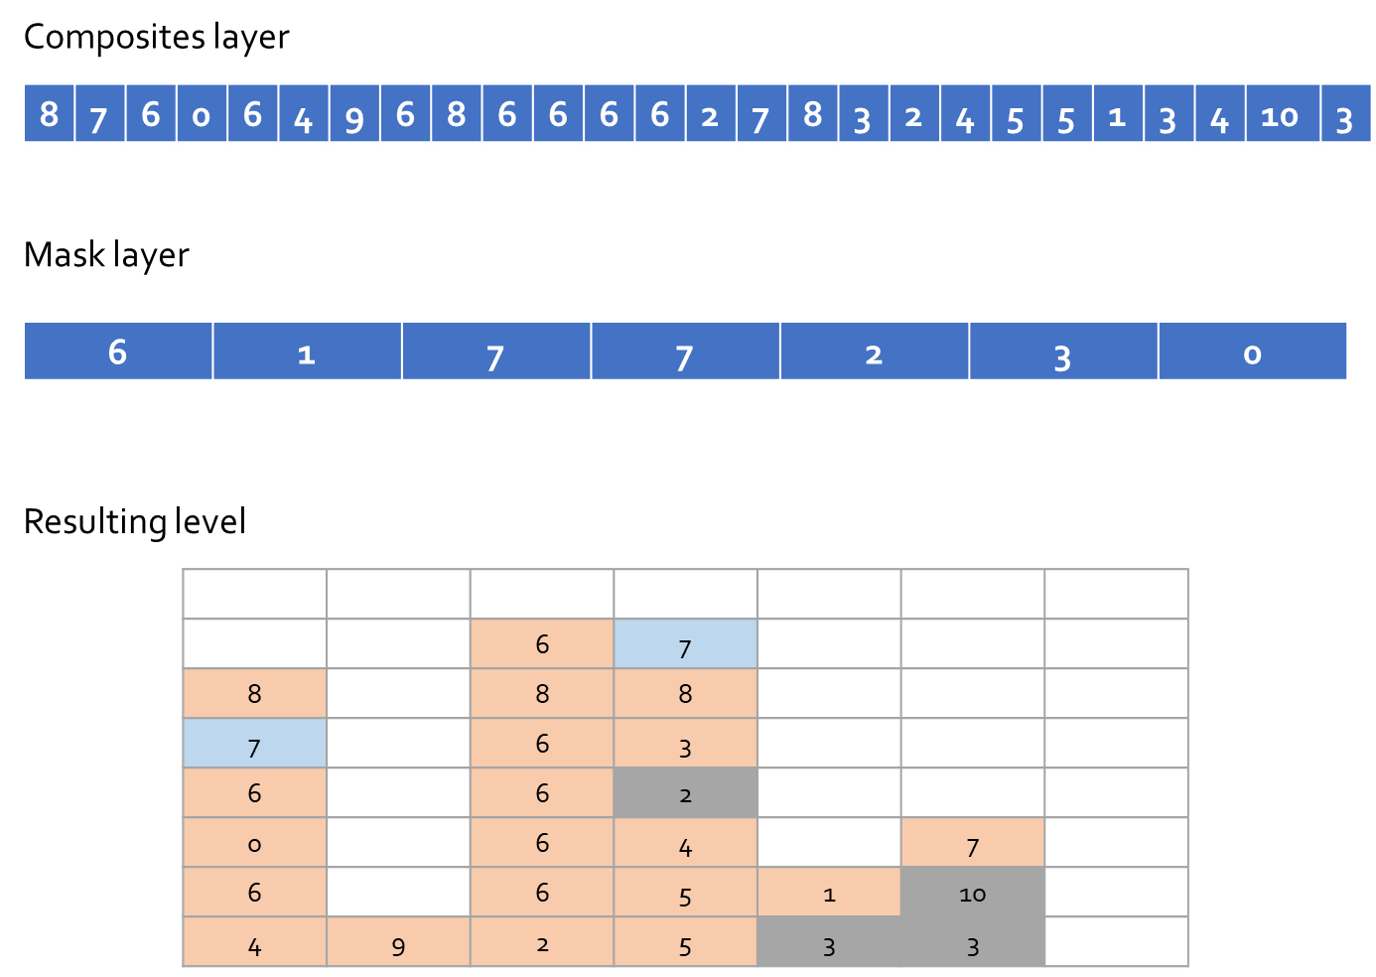
\includegraphics[width=0.9\textwidth]{img/layer12_combine.png}
  \caption{Ejemplo de la combinación de capas de un individuo}
  \label{figure:individual_representation}
\end{figure}

En la figura \ref{figure:individual_representation} muestra la estructura de los
componentes de un individuo, un individuo es representado por \textit{2} capas
diferentes en forma de lista, la primera es la capa de compuestos, está capa se
muestra la lista de compuestos que representan a un individuo, está listas puede
variar en tamaño dependiendo de si durante las operaciones de mutación se le
agregaron o quitaron elementos al individuo, de igual manera cómo se explicó en
el la sección \ref{section:composite_creation} cada valor de la lista representa
no una pieza del juego sino uno de los compuestos que se crean antes de iniciar
el algoritmo o aquellos que se agregan durante el mismo en caso de haber.

La segunda parte que compone la representación del individuo es la máscara, cómo
se explica en la sección \ref{subsection:ruleofthirds} la idea detrás del uso de
está máscara es la de generar estructuras utilizando la lista de compuestos del
individuo, en esta misma sección se presentó una propuesta de crear máscaras en
donde se denotará la forma que se quería que tuviera un individuo particular,
aplicando estás estructuras en los individuos generaba los resultados esperados,
siendo el caso niveles en donde la distribución de los compuestos crearan formas
diferentes cómo castillos, torres, casas o diferentes figuras, sin embargo
utilizar está tipo de estructuras no permitía que el algoritmo lograra
evolucionar, sino que simplemente encontraría la mejor combinación de
piezas-máscara en determinado momento, por esto se optó por utilizar la
generación de máscaras que se muestra en la figura
\ref{figure:individual_representation} y que fue explicado en la sección
\ref{section:ind_generation} la cual únicamente muestra una determinada cantidad
de piezas a asignar en posiciones diferentes del nivel, esto permite tener mejor
diversidad en los individuos creados.

Al momento de combinar ambos componentes del individuo se obtiene un resultado
similar al mostrado en la parte inferior de la imagen en donde los compuestos se
organizan en manera de cola, es decir el primer elemento en la lista será el
primero en ser colocado, una vez que se definen cuales elementos serán colocados
en cada columna el sistema calcula la altura total de cada compuesto y
comenzando desde la parte inferior coloca un compuesto en el nivel, después
calcula la distancia desde la parte superior del mismo hasta la parte central
del siguiente para colocarlo de tal forma que al comenzar la simulación no
aparezcan en caída libre, sino que aparezcan una pieza sobre otra, de esta manera
se previenen problemas de balance al permitir que las piezas caigan y
reboten en direcciones que provocaran que las estructuras terminen por caer
totalmente, en la misma imagen se aprecian cuadros de diferentes colores, estos
mismos representan el material del cual está construido cada compuesto cómo se
explico en la sección de mutación anterior.

Finalmente, una vez que se tiene la información anterior definida se procede a
realizar una búsqueda de los lugares en donde aparecerán los enemigos del juego,
la manera en cómo se define dónde pueden aparecer estos es mediante una función
que revisa los compuestos que existen en el nivel, cuando un compuesto cumple
con ciertas características se permite que uno de los enemigos pueda ser
colocado en la parte central o superior del mismo, al iniciar este método se
busca aquellos que cumplen está característica y se ordenan en una lista
auxiliar, después de manera pseudo-aleatoria se decide la cantidad de enemigos
que tendrá el nivel, de acuerdo a este valor se seleccionan \textit{x} cantidad
de posiciones para colocar a los enemigos donde \textit{x} es el valor de
enemigos requeridos, una vez se definió en donde estarán colocados estos
enemigos se regresa una lista con las coordenadas \textit{x} y \textit{y} de las
mismas.

Mediante la combinación de los enemigos con el genotipo construido de un
individuo se obtiene el nivel a mostrar en el juego, una representación de esto
se muestra en la figura \ref{figure:ind_representation_plus_pigs} en donde al
genotipo armado de acuerdo a los puntos anteriormente mencionados se le agrega el
listado de posiciones de los enemigos, en este caso los enemigos son
representados por un color verde en las posiciones en donde estarán, finalmente
esto permite tener la estructura de los niveles completa, está información se
utiliza al momento de generar los archivos de \textit{XML} los cuales en el
software de simulación generaran una vista de los mismos cómo se muestra en la
esquina inferior derecha de la misma imagen. 

\begin{figure}
  \centering
  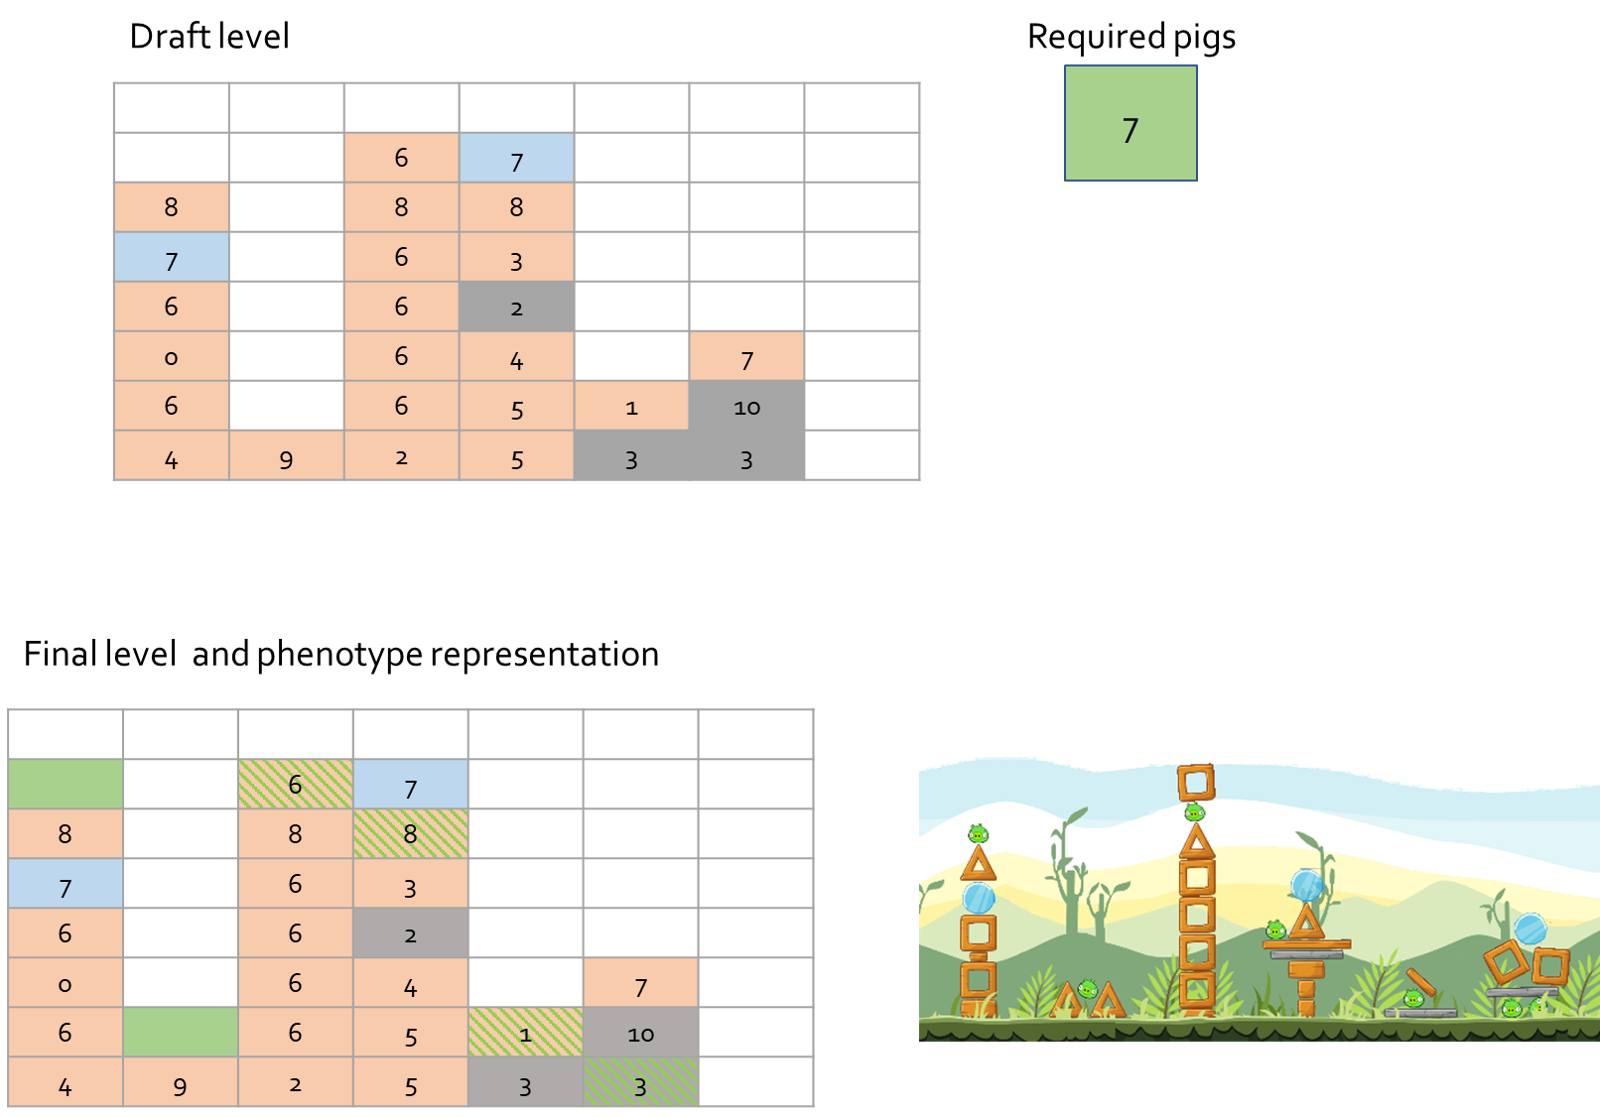
\includegraphics[width=0.9\textwidth]{img/layer123_combine.png}
  \caption{Ejemplo de la combinación de un genotipo armado de la figura \ref{figure:individual_representation} con la colocación de enemigos}
  \label{figure:ind_representation_plus_pigs}
\end{figure}

\subsection{Cálculo de fitness}
\label{subsection:fitness_calculation}

Cuando los individuos pasan por el proceso de simulación se genera un archivo en
formato \textit{XML} que contiene los resultados de los compuestos que fueron
puestos en los archivos antes de la simulación con la diferencia de que estos
archivos contienen la información del ultimo estado de los mismos compuestos al
terminar dicha simulación es decir se obtiene un listado de piezas y enemigos con
la información de sus posiciones \textit{x} y \textit{y} así cómo del angulo con
en el cual quedaron al concluir la simulación, además de esto se entrega la
información de la velocidad promedio de movimiento que tuvieron.

Está información permite conocer las imperfecciones que tuvieron los niveles al
concluir las simulaciones, para mejorar la evaluación obtenida que determina la
aptitud de los individuos se toma en cuenta una evaluación de dos fases la
primera fase tiene que ver con la estabilidad de los individuos y se evalúa en
base a dos métricas:
\begin{enumerate}
    \item La cantidad de piezas que no son destruidas durante la simulación.
    \item Las posiciones finales de dichas piezas al terminar la simulación.
\end{enumerate}

Para poder realizar el cálculo de las piezas presentes antes y después de la
simulación se utiliza la información de las piezas anteriormente mencionada, sus
posiciones tanto \textit{x} cómo \textit{y} así cómo del angulo de las mismas, a
está información se le agrega un indicador de posición para poder compararlo con
los datos del mismo indicador para las funciones siguientes, está listado de
información se realiza también antes de la simulación con el fin de tener datos
con los cuales comparar, una vez que se tienen los datos se procede a realizar
el proceso de cálculo de fitness, para calcular le diferencia de piezas se
compara la cantidad de elementos en ambas, debido que al momento de caer de
alturas grandes algunos elementos tienden a romperse entonces la cantidad de
elementos después de la simulación podrá ser menor, para obtener el primer valor
se realizara un cálculo para obtener un valor entre \textit{0} y \textit{100}
que define la calificación en forma de porcentaje del total de piezas que se
salvaron en la simulación es decir si antes de la simulación se tenía un total
de \textit{10} piezas y al terminar la simulación en el archivo correspondiente
solo existen \textit{5} entonces el individuo tendrá una calificación de
\textit{50\%} debido a que solo la mitad de las piezas no fueron destruidas.

El segundo valor toma se utiliza para definir si los conjuntos que no se
destruyeron se lograron mantener los más estábles posible, esto se calcula
mediante el uso de dos fórmulas mostradas en las formulas
\ref{equation:error_pos} y \ref{equation:error_ang} mediante el uso de estás
formulas se comprueba si las piezas se lograron o no mantener en sus posiciones
originales, en los casos donde las piezas no se hayan destruido se utilizan
estás fórmulas para revisar si las posiciones y ángulos de inicio y final de la
simulación son los mismos, en caso de que así sea entonces no se realizan
modificaciones al fitness obtenido previamente, en caso contrario se obtiene una
penalización al fitness equivalente a una tercera parte del valor de porcentaje
por una pieza si se movió de posición y otra tercera parte si su angulo cambio.

\begin{equation}
    \begin{split}
      error_{xy} = & 
      \begin{Bmatrix}
        0 \qquad si \qquad 0.08 > d \\ 
        \frac{100}{longitud\_piezas} * -0.33 \qquad si \qquad 0.08 < d
      \end{Bmatrix} \\
       d & = \sqrt{(x_2 - x_1)^2 + (y_2 - y_1)^2}
    \end{split}
    \label{equation:error_pos}
\end{equation}

\begin{equation}
    \begin{split}
      error_{r} = & 
      \begin{Bmatrix}
        0 \qquad si \qquad -5 < r < 5 \\ 
        \frac{100}{longitud\_piezas} * -0.33 \qquad si \qquad 0.08 < d
      \end{Bmatrix} \\
       r & = \left | rotacion_o \right | - \left | rotacion_f \right |
    \end{split}
    \label{equation:error_ang}
\end{equation}

Por otro lado, la segunda fase de la evaluación busca tener más diversidad en los
individuos, esto es que tan \textit{nuevos} y \textit{diferentes} logran ser, la
manera en cómo se propone realizar está evaluación de diversidad es mediante el
uso de las métricas:
\begin{enumerate}
    \item La diversidad de las piezas utilizadas en los individuos
    \item El resultado de la función de entropía con las piezas utilizadas.
    \item La distancia \textit{Hamming} del mismo conjunto de piezas.
\end{enumerate}

Para evaluar la diversidad de los elementos primero se realiza un cálculo de los
diferentes compuestos que integran a un individuo, para la evaluación de está
parte se toma en cuenta la diversidad que logra tener el individuo, en donde el
utilizar diferentes compuestos de la lista total permite tener una mejor
calificación, esto es debido que mientras más compuestos sean utilizados los
niveles que se pueden generar serán diversos entre sí.

Posterior a esto se realiza un cálculo de la entropía de un individuo, el
cálculo de entropía es utilizado en la teoría de información para calcular el
nivele de desorden o incertidumbre en los individuos, la fórmula que se utiliza
para esto se muestra en \ref{equation:entropy}

\begin{equation}
  s = -\sum _{i} P_i log P_i
  \label{equation:entropy}
\end{equation}
\myequations{Ecuación de entropía}

La manera en cómo la entropía es utilizada en este proyecto es para determinar
si un individuo se vuelve \textit{"aburrido"} o \textit{"interesante"} la manera
en cómo se define este concepto para el individuo es mediante la medición de las
piezas semejantes en el mismo, de acuerdo a esto si la cantidad y tipos de
compuestos se repiten demasiado en el individuo entonces el individuo tiene
entropía baja o en otras palabras se vuelve \textit{"aburrido"} y
\textit{monotono}, es decir si se tiene entropía baja entonces significa que los
compuestos utilizados son mayormente iguales dentro del individuos los cual
generará un nivel demasiado simple a diferencia de si se tiene entropía alta
significa que la cantidad de compuestos diferentes es alta los cual generara
niveles con formas un poco más impredecibles.

\begin{equation}
d = min \begin{Bmatrix} $ d(x, $ y)$ : $ x, $ y $ \epsilon $ C, si $ x \neq y $ entonces 1 $ sino $ 0 $ \end{Bmatrix}
\label{equation:hamming}
\end{equation}
\myequations{Ecuación de la distancia Hamming}

Una vez que se obtuvo el cálculo de la entropía del individuo se procede a
obtener la distancia \textit{Hamming} del mismo, de manera sencilla la
\textit{distancia de hamming} (Hamming distance en Inglés) representa el calculo
realizado en dos cadenas de valores en donde el punto es encontrar el valor
mínimo de sustituciones necesarias para cambiar una cadena a otra, visto de otra
manera, la \textit{distancia de hamming} se encarga de encontrar la distancia
más corta entre dos cadenas, la manera en cómo funciona está función se muestra
en la formula \ref{equation:hamming}, en esta misma ecuación los objetos
\textit{x} y \textit{y} representan listas, en este caso se manejan listas de
valores boléanos es decir listas de valores \textit{0} y \textit{1}, una
explicación más simple se presenta en la función \ref{equation:hammin_example}.

\begin{equation}
  \begin{split}
    C = & \begin{Bmatrix} a, b, c \end{Bmatrix} \\
     & a = (00000) \\
     & b = (10110) \\
     & c = (01011) \\
     d(a, b) & = 3 \qquad d(a, c) = 3 \qquad d(b, c) = 4
  \end{split}
  \label{equation:hammin_example}
\end{equation}
\myequations{Ejemplo de uso de la distancia de Hamming}

\begin{equation}
  \begin{split}
    error_{r} = & 
    \begin{Bmatrix}
      0 \qquad si \qquad -5 < r < 5 \\ 
      \frac{100}{longitud\_piezas} * 0.5 \qquad si \qquad 0.08 < d
    \end{Bmatrix} \\
     r & = \left | rotacion_o \right | - \left | rotacion_f \right |
    % d(a, b) & = 3 \qquad d(a, c) = 3 \qquad d(b, c) = 4
  \end{split}
  \label{equation:error_ang}
\end{equation}

En esta función se tiene un conjunto de listas representado por \textit{C}, en
este conjunto existen las listas \textit{a, b y c}, para poder encontrar la
\textit{distancia de hamming} de cada par de listas se utiliza la formula
\ref{equation:hamming} esto es, se revisa cada par de elementos de la listas y
se suma \textit{1} si los elementos son diferentes, de está manera se logra
determinar que la cantidad de cambios necesarios para hacer que la lista
\textit{b} se asemeje completamente a la lista \textit{a} es \textit{3} debido a
que solo se requiere cambiar los tres valores \textit{1} en la lista \textit{b},
la razón por la que no es requerido cambiar valores en la lista \textit{a} es
debido a que en la función la segunda lista utilizada es la que se quiere
asemejar a la primera no solamente cambiar una lista a otra.

Al utilizar la distancia de \textit{hamming} se obtiene cómo mencionado
anteriormente la cantidad menor de cambios para asemejar una lista a otra, sin
embargo cómo el fin de sistema es crear niveles que sean diferentes entre si
entonces es posible incluso modificar la evaluación para obtener este valor para
obtener la mayor distancia posible de tal modo que se sabrá cuales individuos
tendrán la tendencia de ser diferentes para generar más diversidad.

\subsection{Seleccion de miembros elite}
\label{subsection:elite_selection}

Finalmente, después de obtener los resultados de aptitud de los individuos se
procede a realizar la selección de aquellos que lograran integrar el grupo de
elite que se utilizara para sustituir miembros de la población al inicio de la
siguiente generación, para realizar esto primero se requiere ordenar todos los
individuos por medio de su respectivo valor de fitness desde el valor más alto
hasta el valor más bajo, posteriormente se toma una determinada cantidad de
individuos iniciando desde el mejor, la cantidad de individuos que se tomaran
para el grupo de elite es una cantidad que se define antes de iniciar el
algoritmo genético.

Una vez que se ha tomado la cantidad de individuos requerida se procede a
integrar estos mismos individuos a el grupo de elite, para realizar la
integración al grupo de elite primero se requiere analizar el estado del grupo,
en caso de que no existan elementos en la lista lo cual solo sucede en la
primera generación, el grupo seleccionado se integra automáticamente a la lista
de elite, después se ordena la lista de acuerdo al valor de aptitud y se corta de
tal manera que la longitud de la lista de elite sea menor o igual a un valor que
se determina antes de iniciar el algoritmo, en caso de que ya existan elementos
en el grupo entonces estos miembros se integran al final de la lista del grupo
elite, se realiza un reordenamiento en la lista en base al valor de aptitud de
los individuos y se corta la lista en caso se ser requerido.

Una vez que se han completado todos los procesos anteriormente explicados el
algoritmo agrega datos de los mejores, los perores y el promedio de los valores
de aptitud de los individuos en listas que sirven para realizar promedios al
final de toda la ejecución del código, además de esto también se guarda
información de los resultados individuales de las funciones de \textit{entropia}
y la \textit{distancia de hamming} con el fin de ver en manera de graficas el
comportamiento del algoritmo bajo los datos que le fueron proveídos al inicio de
la ejecución. Al terminar este proceso de integración de datos se realiza el
ultimo movimiento en la información de la generación siendo este obtenerlos
archivos \textit{XML} de los individuos y guardándolos en una nueva locación con
el fin de mantener un registro del progreso de los individuos durante la
ejecución del algoritmo.
\chapter{Experimentos y Resultados}
\label{chapter:experiments-and-results}

Este capitulo es el encargado de describir los diferentes experimentos
realizados con el sistema, dichos experimentos se realizaron para comprobar la
correcta funcionalidad de lo creado asi como para revisar que efectivamente el
sistema hace lo que fue propuesto en capitulos anteriores, eso es la generacion
de niveles estables y diferentes entre si.

La manera en como se representaran estos resultados sera mediante el uso de dos
graficas, la primera establece los valores de fitness minimos y maximos que se
logran alcanzar durante las generaciones, ademas de esto en la misma grafica se
presenta una linea extra que representa el promedio de los fitness de los mismos
individuos, siguiente de esto se presenta una segunda grafica que representa la
\textit{distancia hamming} minima alcanzada en cada conjunto de individuos
durante las generaciones, como se explico anteriormente esta grafica representa
el valor minimo de cambios entre los conjuntos de listas de genotipos de los
individuos, esta grafica tendra la tendencia de ir reduciendose conforme avanzan
las generaciones debido a que mientras mas se avanza en las generaciones los
elementos elite tenderan a ir apareciendo mas.

La manera en como se define el valor de fitness de los individuos es como se
explica en la seccion \ref{subsection:fitness_calculation} es mediante la
separacion de los dos aspectos de importancia en los niveles, primero la
\textit{estabilidad} que define el comportamiento del genotipo durante la
simulacion y la segunda siendo \textit{diversidad} que define lo \textit{nuevo}
que logran ser los niveles generados.

Los parametros del algoritmo genetico explicados en el capitulo
\ref{chapter:implementation} se muestran en la tabla \ref{table:parametros_ga}.

\begin{table}[ht]
  \caption{Parametros utilizados en el algoritmo genetico}
  \label{table:parametros_ga}
  \centering
  \begin{tabular}{|c|c|}
  \hline
  Parametro & Valor \\
  \hline
  \hline
  Fitness Function & Estabilidad \\ & Diversidad \\
  \hline
  Tamaño de la poblacion & 10 o 20 \\
  \hline
  Numero de Generaciones & 100 o 10 (respectivamente) \\
  \hline
  Criterio de parada & Numero de Generaciones \\
  \hline
  Operador de seleccion & Seleccion por torneo \\
  \hline
  Operador de cruce & Cruce de un punto \\
  \hline
  Porcentaje de cruce & 30\% \\
  \hline
  Operador de mutacion & Mutacion de individuo \\ & Mutacion de compuestos \\ & Mutacion de material \\
  \hline
  Poercentaje de mutacion & 30\% \\
  \hline
  \end{tabular}
\end{table}


El contenido de este capitulo se encargara de mostrar las capacidades de
generacion del sistema propuesto e implementado segun lo mostrado en el capitulo
\ref{chapter:implementation} deacuerdo a las areas explicadas anteriormente.
Cada experimento mostrado se describira en los ambitos de la capacidad de
generar niveles \textit{estables} asi como tambien la capacidad de generar
niveles \textit{diversos}, puesto que se tienen una gran cantidad de indivudos
en las simulaciones entonces para demostrar ambos ambitos se tomaran el
\textit{mejor} y el \textit{peor} del final de cada experimento asi como un
indiviudo aleatorio de la primera generacion, utilizando estos niveles generados
se explicara la manera en como se evoluciono la diversidad de los niveles y
cuales fueron los compuestos que se pueden rescatar de las simulaciones para ser
utilizados en experimentos subsecuentes, para tener un campo nivelado para todos
los experimentos aquellos compuestos que aparecen durante los experimentos no
son reutilizados en otros experimentos subsecuentes.

Todos los experimentos mostrados en esta seccion fueron optimizados durante un
total de 10 generaciones, esto es debido principalmente a que para realizar las
simulaciones se requiere una gran cantidad de tiempo, esto sumado con la
cantidad diferente de indiviudos, en experimentos de 100 generaciones se
utilizaban un total de 10 individuos y para experimentos de 10 generaciones se
utilizo un total de 20, ademas de esto en muchos de los experimentos de 100
generaciones el algoritmo llegaba a un punto de estancamiento generalmente antes
de las primeras 50 generaciones, por tal motivo se decidio reducir la cantidad
de generaciones a 10 pero incrmementar el total de indiviudos para obtener una
mayor diversidad.

Como se explico en el parrafo anterior los experimentos que se presentaran
cubriran las variables de 20 individuos durante un total de 10 generaciones y
utilizando las variables presentadas en la tabla \ref{table:parametros_ga}.
Utilizando estas configuraciones se realizaron un total de [Write number here?]
sin embargo debido a que los resultados mostrados por cada experimentos son
demasiados solo algunos resultados de experimentos seran mostrados.



The experiments cover the following variants in the parameters: 4 agents, 4
rules and 4 individuals; 10 agents, 10 rules and 10 individuals; 20 agents, 20
rules and 20 individuals; and these variants are used to created models for the
following foreign exchange markets: AUD/USD, EUR/GBP, EUR/USD, GBP/USD and
USD/CAD.

A total of 135 experiments were performed, but due to space constraints in this
thesis document, only some of the experiments are shown. Specifically, the
forecasting and interpretation Sections show results for the cases of 4 agents,
4 rules and 4 individuals; 10 agents, 10 rules and 10 individuals; and 20
agents, 20 rules and 20 individuals. Each of the aforementioned cases are
extracted for each of the five foreign exchange markets: AUD/USD, EUR/GBP,
EUR/USD, GBP/USD and USD/CAD. The reader can find the plots and interpretations
for all the experiments performed in the Git repository of this thesis here:
https://github.com/amherag/PhD-Thesis/.

\section{Forecasting the Prices of a Financial Market}
\label{section:forecasting-the-prices-of-a-financial-market}

This Section shows some experiments that have the goal of forecasting different
foreign exchange markets. Different agent-based models were generated using the
parameters indicated in each of the Subsection titles. The datasets used for the
training stage of the model comprehends the prices and timestamps associated to
each of these prices, from Monday, January 28, 2019 5:00:00 PM GMT-08:00, minus
20 hours that are required to generate the initial retracements (see Section
\ref{section:preprocessing-a-financial-market-using-retracements:implementation})
to Sunday, February 3, 2019 8:00:00 PM GMT-08:00. Regarding the datasets used
for the testing stage of the model, the data comprehends the prices and
timestamps associated to each of these prices, from Sunday, February 3, 2019
9:00:00 PM GMT-08:00, minus 20 hours that are required to generate the initial
retracements, to Friday, February 8, 2019 12:00:00 AM GMT-08:00. All the
datasets have a size of 100 data points, and they correspond to the prices of
the foreign exchange markets AUD/USD, EUR/GBP, EUR/USD, GBP/USD and USD/CAD
according to the corresponding experiments Section.

Each of the following Subsections shows five plots: two plots of the
curve-fitting of the optimized model for the training and testing datasets, two
plots of the profits generated by the simulated trades of the optimized models
for the training and testing datasets, and a plot of the error minimization in
the training or optimization stage. The titles of the plots for both the
training and testing stages also include the mean-squared error in parentheses
(denoted by $\epsilon$) for the simulated versus real prices. The profit plots
show the accumulated profits through time in asset units. The minimization plot
shows the mean-squared error obtained by the best individual in each of the
generations.

\newpage

\subsection{AUD/USD 4 Agents, 4 Rules, 4 Individuals}
\label{results:forecast-aud-usd-4agents-4rules-4individuals}

Figure \ref{figure:aud-usd-4agents-4rules-4individuals} shows the plots for the
agent-based model with the worse modelling capabilities for the foreign exchange
market AUD/USD. As can be expected, the model did not achieve good training or
testing profits, although the mean-squared error is considerably low. This can
be a sign of poor generalization capabilities of the model due to the low number
of agents and rules. Additionally, the low number of individuals can provide
cause bad exploration in the genetic algorithm.



\newpage

\subsection{AUD/USD 10 Agents, 10 Rules, 10 Individuals}
\label{results:forecast-aud-usd-10agents-10rules-10individuals}

The plots for the model generated using 10 agents with 10 rules each are shown
in Figure \ref{figure:aud-usd-10agents-10rules-10individuals}. It can be seen
that this model has better modelling capabilities than the 4 agents with 4 rules
each, as it performed better regarding profits in the training stage. However,
both models failed to obtain profits during the testing stage.



\newpage

\subsection{AUD/USD 20 Agents, 20 Rules, 20 Individuals}
\label{results:forecast-aud-usd-20agents-20rules-20individuals}

Despite the increased modelling capabilities and diversity for the genetic
algorithm, the model generated by using 20 agents, 20 rules and 20 individuals
could not outperform the other two models for the AUD/USD. An explanation for
this is that the patterns present in the training dataset are notably different
than those found in the testing dataset, as it can be seen in Figure
\ref{figure:aud-usd-20agents-20rules-20individuals}.







\newpage

\subsection{EUR/GBP 4 Agents, 4 Rules, 4 Individuals}
\label{results:forecast-eur-gbp-4agents-4rules-4individuals}

Figure \ref{figure:aud-usd-20agents-20rules-20individuals} shows the plots for
the 4 agent, 4 rules, 4 individuals model. One can see that both profit plots
show bad performance. Although this is expected from this configuration, it can
also be seen that the model struggled in obtaining a simulation that resembled a
close representation of the real market, especially if it is compared to the 4
agents, 4 rules and 4 individual model for the AUD/USD market (see Figure
\ref{figure:eur-gbp-20agents-20rules-20individuals}).



\newpage

\subsection{EUR/GBP 10 Agents, 10 Rules, 10 Individuals}
\label{results:forecast-eur-gbp-10agents-10rules-10individuals}

An interesting situation is presented in the plots in Figure
\ref{figure:eur-gbp-10agents-10rules-10individuals}. The profit plots are
identical in shape than the plots in Figure
\ref{figure:eur-gbp-4agents-4rules-4individuals}. The only inconsistency is the
magnitude of the trades, as the agents in the previous model traded more units
than the agents in this model.



\newpage

\subsection{EUR/GBP 20 Agents, 20 Rules, 20 Individuals}
\label{results:forecast-eur-gbp-20agents-20rules-20individuals}

Although the model generated with these parameters performed well in the
training stage, as seen in Figure
\ref{figure:eur-gbp-20agents-20rules-20individuals}, it can be seen that the
model performed badly in the testing stage. However, it is worth mentioning that
the model performed well in the first 18-20 hours of the testing stage.






\newpage

\subsection{EUR/USD 4 Agents, 4 Rules, 4 Individuals}
\label{results:forecast-eur-usd-4agents-4rules-4individuals}

This model can be seen how badly it performed in the testing stage, as shown in
Figure \ref{figure:eur-usd-4agents-4rules-4individuals}. However, it performed
well in the training stage. It must also be noted that a bad performance can be
expected due to the differences in the patterns between the training and testing
datasets.



\newpage

\subsection{EUR/USD 10 Agents, 10 Rules, 10 Individuals}
\label{results:forecast-eur-usd-10agents-10rules-10individuals}

The plots in Figure \ref{figure:eur-usd-10agents-10rules-10individuals}
demonstrate an improvement regarding the curve-fitting capabilities of the model
compared to the previous model for the EUR/USD market. This is surprising, given
the differences in patterns between the two datasets. Additionally, it can be
noted that the model performed well in both the training and testing stages,
despite the model performing badly in the last hours of the testing stage.



\newpage

\subsection{EUR/USD 20 Agents, 20 Rules, 20 Individuals}
\label{results:forecast-eur-usd-20agents-20rules-20individuals}

The model represented by the plots in Figure
\ref{figure:eur-usd-20agents-20rules-20individuals} is seen to have performed
badly in both the training and testing stages. A possible explanation for this
behavior is that more generations would be required in order for the model to
extract a generalization of the market, as a consequence of the high number of
agents and rules.






\newpage

\subsection{GBP/USD 4 Agents, 4 Rules, 4 Individuals}
\label{results:forecast-gbp-usd-4agents-4rules-4individuals}

As expected from a model with poor modelling capabilities, the profit plots in
Figure \ref{figure:gbp-usd-4agents-4rules-4individuals} show that the model was
not able to simulate the patterns of the GBP/USD market.



\newpage

\subsection{GBP/USD 10 Agents, 10 Rules, 10 Individuals}
\label{results:forecast-gbp-usd-10agents-10rules-10individuals}

In the case of this model for the GBP/USD market, a remarkable performance can
be noticed in Figure \ref{figure:gbp-usd-10agents-10rules-10individuals} in the
profit plots for both the training and testing stages.



\newpage

\subsection{GBP/USD 20 Agents, 20 Rules, 20 Individuals}
\label{results:forecast-gbp-usd-20agents-20rules-20individuals}

In contrast to other models using 20 agents with 20 rules each, the model
represented by the plots in Figure
\ref{figure:gbp-usd-20agents-20rules-20individuals} is shown to perform well in
both the training and testing stages regarding the accumulated profits, although
the profits do not reach a similar magnitude as the previous model.









\newpage

\subsection{USD/CAD 4 Agents, 4 Rules, 4 Individuals}
\label{results:forecast-usd-cad-4agents-4rules-4individuals}

The plots in Figure \ref{figure:usd-cad-4agents-4rules-4individuals} present an
interesting situation: the model seems to perform badly regarding profits in the
training stage, but not in the testing stage. This behavior is clearer after
examining the plots of the training and testing datasets: one exhibits a
downtrend market direction, while the other shiftes to a clear uptrend. The
model learned how to perform badly in a downtrend market, but it performed well
in the testing stage because of the shift in direction.



\newpage

\subsection{USD/CAD 10 Agents, 10 Rules, 10 Individuals}
\label{results:forecast-usd-cad-10agents-10rules-10individuals}

In contrast to the previous model, the model represented by the plots shown in
Figure \ref{figure:usd-cad-10agents-10rules-10individuals} performs badly in the
testing stage, most likely because of the nature of the training dataset which
sharply contrasts with the nature of the testing dataset.



\newpage

\subsection{USD/CAD 20 Agents, 20 Rules, 20 Individuals}
\label{results:forecast-usd-cad-20agents-20rules-20individuals}

The model represented by the plots in Figure
\ref{figure:usd-cad-20agents-20rules-20individuals} performs similarly to the
previously discussed model. The explanation behind this behavior should be the
same as the one mentioned in the previous Subsection.





\newpage

\section{Extracting Insights about a Financial Market}
\label{section:extracting-insights-about-a-financial-market}

This Section shows interpretations of two different foreign exchange markets
obtained by examining the agents in the agent-based models generated for the
experiments shown in Section
\ref{section:forecasting-the-prices-of-a-financial-market}. Only the two markets
are presented in this Section as they are enough to demonstrate their use. The
rest of the interpretetations for the markets described in Section
\ref{section:forecasting-the-prices-of-a-financial-market} can be found in
Appendix \ref{app:market-interpretations}, and the full list of interpretations
for all the experiments performed can be found in the git repository of this
thesis document. The interpretations
consist of a series of sentences, where each give a summary of the profits,
perceptions, hesitancy and actions of groups of agents. Considering the
following sentence: ``3 agents — with an average profit of 68 units — perceived
in 85\% of the market that a weak resistance above current price — with a
hesitancy of 0.147 — is a signal to sell — with a hesitancy of 0.079.'', one can
draw the following conclusions about 3 agents in a community of agents: their
average profit in a dataset is of 68 units; in 85\% of the data points in the
dataset, they perceived that a price area with a low weight above the current
price is a signal to sell; after perceiving a low weight price area, they add
some hesitancy or doubt to their perception, and then they decide to sell, but
this decision has also some hesitancy or doubt. Hesitancy or doubt (see Section
\ref{section:using-the-agent-based-model-to-generate-insights-about-a-financial-market})
in this case is an indicative of how significant the perception has to be in
order to be indeed perceived as a low weight price area, and how many units are
actually traded; it can be seen as penalties to the agent's perception and
action.

The following interpretations show five sentences for the training stage of the
model and five sentences for the testing stage. These only represent excerpts of
the generated interpretations; it was decided for them to be truncated due to
space constraints in this thesis document, but the reader can find the full
interpretations in this thesis' Git repository. In order to obtain these five
sentence excerpts, all the generated sentences were ordered by the number of
agents and then by the number of units in profits. This way the sentences show
where the most number of agents in the community of agents coincided in their
perceptions and decisions, and then show what situations were the more
profitable.

%% Interpretations for the five foreign exchange markets AUD/USD, EUR/GBP, EUR/USD,
%% GBP/USD and USD/CAD are included. Each of these markets show interpretations for
%% the models with the following variants in parameters: 4 agents, 4 rules and 4
%% individuals; 10 agents, 10 rules and 10 individuals; 20 agents, 20 rules and 20
%% individuals.

\subsection{AUD/USD 4 Agents, 4 Rules, 4 Individuals}

One can see in the first sentence of the training set that 3 agents decided to
trade when a weak resistance is presented above the current price. In the
training stage these agents were not profitable, while in the testing stage they
were profitable. This indicates that this pattern is not as reliable as, for
example, the one presented in the second sentence in the training set, where
agents decided to buy when they perceived a weak resistance nearby the current
price. This behavior showed to also be profitable in the testing stage, as is
shown in the fourth sentence of the corresponding set.

\subsubsection{Training}

{\small
  \begin{itemize}
  \item 3 agents — with an average profit of -68 units — perceived in 68\% of
    the market that a weak resistance above current price — with a hesitancy of
    0.147 — is a signal to sell — with a hesitancy of 0.079.
  \item 2 agents — with an average profit of 280 units — perceived in 46\% of
    the market that a weak resistance nearby current price — with a hesitancy of
    0.133 — is a signal to buy — with a hesitancy of 0.097.
  \item 2 agents — with an average profit of 280 units — perceived in 22\% of
    the market that a moderate resistance above current price — with a hesitancy
    of 0.15 — is a signal to buy — with a hesitancy of 0.113.
  \item 2 agents — with an average profit of 38 units — perceived in 56\% of the
    market that a weak resistance below current price — with a hesitancy of
    0.246 — is a signal to buy — with a hesitancy of 0.094.
  \item 2 agents — with an average profit of -41 units — perceived in 56\% of
    the market that a weak resistance below current price — with a hesitancy of
    0.009 — is a signal to sell — with a hesitancy of 0.132.
  \end{itemize}
}

\subsubsection{Testing}

{\small
  \begin{itemize}
  \item 3 agents — with an average profit of 68 units — perceived in 85\% of the
    market that a weak resistance above current price — with a hesitancy of
    0.147 — is a signal to sell — with a hesitancy of 0.079.
  \item 2 agents — with an average profit of 352 units — perceived in 47\% of
    the market that a moderate resistance below current price — with a hesitancy
    of 0.134 — is a signal to sell — with a hesitancy of 0.151.
  \item 2 agents — with an average profit of 323 units — perceived in 6\% of the
    market that a strong resistance below current price — with a hesitancy of
    0.098 — is a signal to sell — with a hesitancy of 0.024.
  \item 2 agents — with an average profit of 323 units — perceived in 55\% of
    the market that a weak resistance nearby current price — with a hesitancy of
    0.04 — is a signal to sell — with a hesitancy of 0.138.
  \item 2 agents — with an average profit of 309 units — perceived in 0\% of the
    market that a strong resistance above current price — with a hesitancy of
    0.127 — is a signal to sell — with a hesitancy of 0.14.
  \end{itemize}
}

\subsection{EUR/GBP 4 Agents, 4 Rules, 4 Individuals}

An interesting situation in these sets of interpretations is that the only
sentence in the training set that signals an actual trade action is among the
most profitable interpretations in the testing stage -- but with a 0\% of
perception in the market. This can also be seen as a signal to not follow the
behavior presented by this model, which agrees the profit plots of the model
presented in the previous Section.

\subsubsection{Training}

{\small
  \begin{itemize}
  \item 3 agents — with an average profit of 60 units — perceived in 56\% of the
    market that a weak resistance above current price — with a hesitancy of
    0.094 — is a signal to hold the current position — with a hesitancy of
    0.029.
  \item 3 agents — with an average profit of 31 units — perceived in 36\% of the
    market that a moderate resistance nearby current price — with a hesitancy of
    0.126 — is a signal to hold the current position — with a hesitancy of
    0.194.
  \item 3 agents — with an average profit of -44 units — perceived in 13\% of
    the market that a strong resistance below current price — with a hesitancy
    of 0.044 — is a signal to hold the current position — with a hesitancy of
    0.152.
  \item 2 agents — with an average profit of 105 units — perceived in 13\% of
    the market that a strong resistance below current price — with a hesitancy
    of 0.114 — is a signal to sell — with a hesitancy of 0.102.
  \item 2 agents — with an average profit of 105 units — perceived in 42\% of
    the market that a weak resistance nearby current price — with a hesitancy of
    0.105 — is a signal to hold the current position — with a hesitancy of
    0.048.
  \end{itemize}
}

\subsubsection{Testing}

{\small
  \begin{itemize}
  \item 3 agents — with an average profit of 34 units — perceived in 79\% of the
    market that a weak resistance above current price — with a hesitancy of
    0.094 — is a signal to hold the current position — with a hesitancy of
    0.029.
  \item 3 agents — with an average profit of 18 units — perceived in 33\% of the
    market that a moderate resistance nearby current price — with a hesitancy of
    0.126 — is a signal to hold the current position — with a hesitancy of
    0.194.
  \item 3 agents — with an average profit of -23 units — perceived in 0\% of the
    market that a strong resistance below current price — with a hesitancy of
    0.044 — is a signal to hold the current position — with a hesitancy of
    0.152.
  \item 2 agents — with an average profit of 60 units — perceived in 0\% of the
    market that a strong resistance below current price — with a hesitancy of
    0.114 — is a signal to sell — with a hesitancy of 0.102.
  \item 2 agents — with an average profit of 60 units — perceived in 57\% of the
    market that a weak resistance nearby current price — with a hesitancy of
    0.105 — is a signal to hold the current position — with a hesitancy of
    0.048.
  \end{itemize}
}

\section{Comparison with other Works}
\label{section:comparison-with-other-works}

This Section presents a set of works that share many similarities to the work
proposed in this thesis and that are comparable to it. Table \ref{table:results}
shows five different works that focus on forecasting a financial market and
yield a rate of return. The table columns show the work reference and its
authors; the technique used to perform the forecasting; the optimization
algorithm used, if any; the financial market type used; the percentage of profit
or rate of return after a number of trades; and the standard deviation for the
aforementioned rate of return. The purpose of this table is to showcase what are
normal values of performance when forecasting financial markets and not to
provide a concise comparison for the proposed method, as many factors do not
match among the different works shown in the table: the size of the dataset used
for training, the technique used, the parameters of the optimization algorithm,
the number of trades performed, the type of the financial market,
etc. Furthermore, the results shown in this Chapter had the purpose of
demonstrating how the proposed method behaves using different parameters and not
to obtain the maximum possible rate of return.

\begin{table}[ht]
\caption{Performance of different approaches to financial market forecasting}
\label{table:results}
\centering
\begin{tabular}{|c|c|c|c|c|c|}
\hline
Work                                         & Technique                  & Optim. Alg. & Market Type              & ROR & SD \\
\hline
\hline
\cite{Fernandez-Blanco2008} & TI            & Genetic algorithm         & Stock             & 76.13\%     & 14.15\%            \\
\hline
\cite{Korczak2015}          & Fuzzy MAS        & -                      & ForEx & 32.77\%     & 109.09\%           \\
\hline
\cite{Korczak2016}          & Fuzzy MAS        & Genetic algorithm      & ForEx & 223.08\%    & 385.7\%            \\
\hline
\cite{Barbosa2010}          & Ensemble MAS     & -                      & ForEx & 27.78\%     & 12.43\%            \\
\hline
\cite{Escobar2013}          & Fuzzy TI         & -                      & Stock             & 7.35\%      & 6.9\%              \\
\hline
Thesis             & Fuzzy MAS        & Genetic algorithm      & ForEx & 2.15\%      & 38.85\%  \\
\hline
\end{tabular}
\end{table}

The rate of returns shown in Table \ref{table:results} for the proposed method
were obtained by averaging the units of profit for all the models that used a
configuration of 10 agents, 10 rules and 10 individuals for the following
financial markets: AUD/USD, EUR/GBP, EUR/USD, GBP/USD and USD/CAD. These models
were chosen because this configuration showed a good performance, considering
only the results included in this thesis document; other configurations could
have achieved a better performance.
\chapter{Conclusiones y trabajo futuro}
\label{chapter:conclusions-and-future-work}

En las siguientes secciones se presentan las conclusiones a las que se llegaron
durante el desarrollo del proyecto de tesis presentado en este documento, sobre
la manera en cómo se implementaron los aspectos propuestos, así como de los
resultados que se lograron obtener mediante el uso de estas propuestas. Así
mismo dentro de la última sección de este capítulo se discuten y proponen
diferentes métodos que pueden ser implementados a futuro para mejorar los
resultados obtenidos, rutas de investigación que se teorizaron podrían funcionar
así como aspectos que requieren de mejorar para un funcionamiento más fluido del
sistema.

\section{Conclusiones}
\label{section:conclusions}

Esta tesis presenta un método novedoso para la generación de niveles del juego de
Angry Birds apoyándose en las mecánicas de la evolución genética y de tomando
aspectos de open-ended evolution. El sistema que se logró generar cuenta con las
capacidades para generar estructuras compuestas utilizando elementos básicos del
juego, además que de que debido a la manera en cómo fue programado es posible
modificar los módulos de clases sin requerir modificaciones enormes en el código
fuente, por ejemplo, es posible realizar modificaciones a las funciones de
selección y mutación que se reflejen de manera rápida en el sistema al realizar
las simulaciones de igual manera el sistema de evaluación se puede mejorar ya
sea cambiando las métricas de evaluación propuestas o agregando nuevas según sea
requerido.

Para fines de este proyecto el sistema fue probado con el simulador de Science
Birds utilizando todos los puntos propuestos en la sección
\ref{chapter:proposed-method} y se obtuvieron resultados como los mostrados en
la sección \ref{chapter:experiments-and-results}, sin embargo, una de las ideas
en el desarrollo de este proyecto es el de permitir la adaptabilidad en el
sentido de que se espera que siempre y cuando un caso de estudio particular es
decir un juego diferente tenga niveles que puedan ser descompuestos hasta las
expresiones mínimas, es decir los bloques de construcción que permitirán generar
un nivel será posible en teoría utilizar este mismo sistema para generar niveles
en otros juegos simplemente ajustando algunas variables que permitan comparar
los compuestos a fin de obtener los resultados esperados.

La implementación mostrada en la sección \ref{chapter:proposed-method} muestra
cómo se explicó anteriormente las ideas que se consideran fueron las mejores
para desarrollar el sistema, sin embargo, aquellas mostradas como propuestas
anteriores demuestran los cambios por los cuales el sistema tuvo que pasar para
poder obtener lo que consideramos como el "mejor" en términos de lo que se
proponía lograr, así como estos mismos métodos podían aproximar resultados a los
obtenidos en el sistema final pueden existir diferentes técnicas que no se
exploraron a detalle que logren obtener resultados iguales o inclusive mejores,
ejemplos como los presentados en la sección \ref{chapter:related-work}
demuestran que diferentes personas lograron tener diferentes métodos de atacar
esta problemática, desde el uso de sistemas inteligentes o sistemas
auto-adaptables, mediante el uso de estas diferentes técnicas se observa una
gran diversidad de resultados, en el caso de este sistema los métodos que se
opina pueden sustituir al algoritmo genético son técnicas basadas en búsquedas
meta-heurísticas debido a la naturaleza del sistema.

Uno de los puntos tratados durante los capítulos \ref{chapter:implementation}
y \ref{chapter:experiments-and-results} es el problema relacionado con el tiempo
de simulación, debido a que los niveles generados requieren ser evaluados dentro
de los parámetros del juego como tal se requiere que el juego se ejecute y
evalué cada nivel uno a la vez, esto provoca que los tiempos de simulación sean
tardados debido a que cada nivel requiere ser simulado durante 10 segundos con
el fin de que las estructuras generadas tengan tiempo de reaccionar bajo la
gravedad, si están mal acomodadas caerán y si están correctamente acomodadas se
mantendrán de pie o balanceadas además de este tiempo de simulación se toma
también en cuenta el tiempo que tarda en escribir los resultados de cada nivel
en sus respectivos archivos eh inclusive el tiempo que el software de simulación
tarda en ser ejecutado, este punto fue uno de los obstáculos más grandes en el
sistema debido a que solo analizar si un cambio funcionaba bien podía tardar
mucho, sin embargo, este tiempo se reduce considerablemente cuando se trabaja en
generaciones diferentes a la inicial debido a que en generaciones subsecuentes
solo se programó que simulara aquellos individuos que fueron generados, gracias
a que este fue un obstáculo que se tuvo que mantener en el sistema se lograron
adaptar partes del sistema para realizar las simulaciones de manera más fluida y
no requerir de volver a ejecutar una simulación para analizar el flujo de los
datos lo cual permitió encontrar errores más rápidamente.

\section{Trabajo futuro}
\label{section:future-work}

Las conclusiones descritas previamente proveen dan un entendimiento de los
obstáculos que por los cuales se tuvo que pasar para poder completar el
proyecto, el problema y posible solución tratados en las conclusiones sobre las
simulaciones generadas es el tiempo desperdiciado debido al uso del software de
simulación, debido a que las simulaciones requieren de este software para poder
obtener los resultados es necesario encontrar una manera en la cual se pueda
estimar mediante el uso de fórmulas las posiciones en las cuales terminaran los
elementos del nivel, considerando que el juego como tal tiene un sistema de
gravedad que provoca que las piezas caigan al suelo debería de ser posible
calcular u obtener el valor de gravedad utilizada para desarrollar un sistema
capaz de calcular el movimiento de las piezas considerando también la
interacción de las piezas unas con otras, así como las resistencias con las que
cuentan.

El ámbito de la evaluación de los individuos es uno de los principales que puede
ser mejorado o modificado, esto es debido a que las funciones que se utilizaron
para la evaluación en esta tesis son las que se consideraron óptimas para la
problemática tratada, de acuerdo a lo que se requiera obtener es posible
modificar la manera en cómo se obtienen los resultados de aptitud de los
individuos, en el caso de lo que se utilizó para el desarrollo del proyecto es
posible modificar los cálculos de los resultados de estabilidad, en este caso lo
que se esperaba obtener es el valor más cercano a 100 para cada individuo en
donde 100 representaba que ninguno de los elementos que conformaban el nivel se
destruyeron o cayeron, sin embargo, es posible utilizar algunas otras funciones o
cálculos para poder obtener estos resultados inclusive cambiar la manera de
interpretar la estabilidad como el uso de cálculos de aceleración promedio o
movimiento angular de las mismas piezas.

Uno de los ámbitos que también requiere ser tratado es el de la estabilidad de
los niveles generados, es decir el sistema logra generar niveles mediante el
acomodo de los compuestos que se tienen registrados, sin embargo, una de las
maneras en cómo el proceso de evaluación, así como el de simulación puede ser
optimizado un poco mas es mediante el uso de reglas de generación o revisión de
patrones en el ordenamiento de los compuestos en los niveles para poder detectar
áreas en donde se pueda estimar que durante la simulación ciertas estructuras
mal acomodadas debido a los componentes básicos que utilizan puedan causar que
los niveles tengan mal rendimiento, es decir, analizar casos en donde una pieza
en particular seguida de otras desfazadas en sus coordenadas \textit{x} o
\textit{y} provoquen que los compuestos se caigan, esto podría ser analizado y
prevenido mediante el uso de diferentes mascaras o en caso de que no sea posible
evitarlo retirar los elementos de la simulación a fin de requerir menos tiempo.

Otro de los factores que pueden ser mejorados es el uso de la lógica detrás de
open-ended evolution, debido a que la consideración de este algoritmo es de
tener una evolución casi infinita y que los niveles del juego se generan una
sola vez al inicio de la evolución realmente no es muy requerido generar nuevos
compuestos de manera continua, pero es posible desarrollar un sistema de
evolución que utilice compuestos resultantes como los mostrados en la sección
\ref{chapter:experiments-and-results} y los integre en una nueva evolución para
combinarlos con componentes básicos e inclusive consigo mismos para generar
nuevos compuestos más complejos que puedan ser integrados a futuras
simulaciones.

Finalmente, un último aspecto que se debe de tomar en cuenta es el número de
experimentos utilizados, como se explicó anteriormente el sistema requería de
mucho tiempo para realizar las simulaciones requeridas por los individuos, esto
inhibió la capacidad de generar una gran cantidad de simulaciones para realizar
comparaciones, sin embargo, con la cantidad actual de resultados obtenidos es
posible validar las capacidades del generador, sin embargo, se requiere realizar
aun más simulaciones utilizando diferentes configuraciones del algoritmo con el
fin de determinar que el sistema es capaz de trabajar correctamente no solo con
el conjunto de configuraciones determinado en la sección de resultados.

%\include{chap8}
%\include{chap9}
\appendix
\setcounter{secnumdepth}{1}
%% This defines the bibliography file (main.bib) and the bibliography style.
%% If you want to create a bibliography file by hand, change the contents of
%% this file to a `thebibliography' environment.  For more information 
%% see section 4.3 of the LaTeX manual.
\begin{singlespace}
\bibliography{main}
\bibliographystyle{ieeetr}
\end{singlespace}

\chapter{} 

\section{Codigo del sitema}
\label{app:code}

\subsection{Codigo principal}
\label{code:main_code}

\begin{minted}[frame=lines, framesep=2mm,baselinestretch=1.2,fontsize=\footnotesize,linenos]{python}
  from __future__ import division, absolute_import                 
  # to avoid integer devision problem
  import datetime 
  import scipy
  import pylab
  #
  import random
  import math
  #
  import datetime
  import time
  from yaspin.yaspin import yaspin
  import os
  import json
  import sys
  import subprocess
  import itertools
  import operator
  import shutil
  import numpy as np
  from copy import deepcopy

  # Local files
  import XmlHelpers as xml
  import Evaluation as Eval 
  from Selection import Selection
  from Mutation import Mutation

  author = "Salinas Hernandez Jaime"
  copyright = "Copyright 2018, Tijuana Institute of Technology"
  credits = ["Dr. Mario García Valdez",""]
  license = "ITT"
  version = "1.4.1"
  date = "May 08, 2019 18:30"
  maintainer = "Salinas Hernandez Jaime"
  email = "jaime.salinas@tectijuana.edu.mx"
  status = "Development"
  t_begin = datetime.datetime.now()
  t_prev = datetime.datetime.now()


  ## Values used for the genetic algorithm
  population = 10         # For now it can only be below 10
  max_gen = 100            # Max number of generations
  fits = [0]              # Variable to save the fitness of each generation
  gen = 0                 # Generation 1
  per_cross = 0.5         # Percentage of cross-over (cross-over operator)
  per_comb = 0.3          # Percentage of combination (combination operator)
  per_mut = 0.8           # Percentage of mutation
  sel_type = 1            # Selection (for crossover) type [ 0: Random - 1: Tournament - TBD]
  cross_type = 0          # Type of cross-over [ 0: One point CO - 1: Random point CO - TBD]
  ind_pieces = 20         # Number of pieces that define an individual
  all_fit = [0]            # Average fitness for all generations
  fit_ham = []           # Average piece length fitness for all generations
  fit_Amov = []           # Average movement fitness for all generations
  max_elite = 1           # Maximum number of elite members in the generation
  elite = []
  best_gen = []
  mu = 0                  # Mean for normal distribution
  sigma = 20              # SD for normal distribution

  min_fit = [0]            # Average fitness for all generations
  max_fit = [0]            # Average fitness for all generations

  ## Data required to create the xml files

  #####################################################################
  ##############< Data required to create the xml files >##############
  #####################################################################

  project_root = os.getcwd()
  json_data = {}
  json_data['all_fit'] = []
  json_data['hamming_avg'] = []
  json_data['min_fit'] = []
  json_data['max_fit'] = []
  ruleset = open("Ruleset/parameters.txt", "r")
  config_param = json.loads(open("ga_parameters.json","r").read())

  game_path = config_param['game_path']
  write_path = config_param['write_path']
  elite_path = config_param['elite_path']
  read_path = config_param['read_path']
  log_path = config_param['log_dir']
  log_base_name = config_param['log_base_name']
  child_level = config_param['child_level']
  child_output = config_param['child_output']

  # For tournament
  game_path_tourney = config_param['game_path_tourney']
  write_path_tourney = config_param['write_path_tourney']
  read_path_tourney = config_param['read_path_tourney']

  # To have a copy of the generations
  level_files_path = config_param['level_files']
  current_gen_folder = config_param['generation']
  sourcefolder = os.path.join(project_root, level_files_path + "/Levels")
  experimentsource = os.path.join(project_root, level_files_path)
  foldername = ''.join(e for e in str(datetime.datetime.now()) if e.isalnum())
  experimentdest = config_param['experiment_results'] + "/" + foldername
  experimentdestination = os.path.join(project_root, experimentdest)

  # Data for the competition
  req_levels = int(deepcopy(ruleset.readline()))
  req_np_combinations = ruleset.readline().split(',')
  for i, e in enumerate(req_np_combinations):
      req_np_combinations[i] = req_np_combinations[i].split()
  req_pigs = ruleset.readline().split(',')

  max_elite = req_levels

  # Clean previous experiment
  #shutil.rmtree(os.path.join(project_root, write_path))
  #shutil.rmtree(os.path.join(project_root, elite_path))
  shutil.rmtree(os.path.join(project_root, level_files_path))

  os.makedirs(os.path.join(project_root, level_files_path), exist_ok=True)

  os.makedirs(os.path.join(project_root, write_path), exist_ok=True)
  os.makedirs(os.path.join(project_root, elite_path), exist_ok=True)
  os.makedirs(os.path.join(project_root, read_path), exist_ok=True)

  os.makedirs(os.path.join(project_root, log_path), exist_ok=True)



  ## "Dictionary" to save the base pieces and structures
  SW_HIDE = 0
  info = subprocess.STARTUPINFO()
  info.dwFlags = subprocess.STARTF_USESHOWWINDOW
  info.wShowWindow = SW_HIDE

  #just for fun making further development easier and with joy
  pi     = scipy.pi
  dot    = scipy.dot
  sin    = scipy.sin
  cos    = scipy.cos
  ar     = scipy.array
  rand   = scipy.rand
  arange = scipy.arange
  plot   = pylab.plot
  show   = pylab.show
  axis   = pylab.axis
  grid   = pylab.grid
  title  = pylab.title
  rad    = lambda ang: ang*pi/180                 #lovely lambda: degree to radian



  # Function to rotate points
  def Rotate2D(pts,cnt,ang=pi/4):
      '''pts = {} Rotates points(nx2) about center cnt(2) by angle ang(1) in radian'''
      return dot(pts-cnt,ar([[cos(ang),sin(ang)],[-sin(ang),cos(ang)]]))+cnt


  # Generation masks
  type_small_l = [[0,0,0,0,0,0,0],
                  [0,0,2,0,0,0,0],
                  [0,0,1,1,0,0,0]]
  type_large_l = [[0,0,3,0,0,0,0],
                  [0,0,2,0,0,0,0],
                  [0,0,1,1,0,0,0]]
  type_small_cube = [[0,0,0,0,0,0,0],
                    [0,0,2,2,0,0,0],
                    [0,0,1,1,0,0,0]]
  type_large_cube = [[0,3,3,3,0,0,0],
                    [0,2,2,2,0,0,0],
                    [0,1,1,1,0,0,0]]
  type_small_floor = [[0,0,0,0,0,0,0],
                      [0,0,0,0,0,0,0],
                      [0,1,1,1,1,1,0]]
  type_large_floor = [[0,0,0,0,0,0,0],
                      [0,0,0,0,0,0,0],
                      [1,1,1,1,1,1,1]]
  type_castle = [[0,0,0,3,0,0,0],
                [2,0,2,2,2,0,2],
                [1,1,1,1,1,1,1]]
  type_house = [[0,0,3,3,0,0,0],
                [0,2,2,2,2,0,0],
                [0,1,1,1,1,0,0]]
  type_towers = [[3,0,3,0,3,0,0],
                [2,0,2,0,2,0,0],
                [1,0,1,0,1,0,0]]

  Mask_List = [
      type_small_l,
      type_large_l,
      type_small_cube,
      type_large_cube,
      type_small_floor,
      type_large_floor,
      type_castle,
      type_house,
      type_towers
  ]

  # Global Piece class and a class for each piece in the game
  class Piece:
      def __init__(self, x, y, r, mat):
          #self.Height = 72
          #self.Width = 72
          self.Material = mat
          self.Dict = []
          self.Valid = True
          self.X = x
          self.Y = y
          self.R = r
          if self.Materials[0] == 0:
              self.Material = "stone"
          if self.Materials[1] == 0:
              self.Material = "ice"
          
      
      def get_edges(self):
          ed_lis = []
          ed_lis.append([self.Width/2 +       self.X,         self.Height/2 +     self.Y])
          ed_lis.append([self.Width/2 +       self.X, 0 -     self.Height/2 +     self.Y])
          ed_lis.append([0 - self.Width/2 +   self.X, 0 -     self.Height/2 +     self.Y])
          ed_lis.append([0 - self.Width/2 +   self.X,         self.Height/2 +     self.Y])
          self.Edges = ed_lis

      def get_points(self, r):
          ang = self.R * pi / 180
          ots = Rotate2D(self.Edges, ar([0 + self.X, 0 + self.Y]), ang)
          self.Points = ots.tolist()
          #print(self.Points)

      def change_material(self, m):
          self.Material = m

      def as_dictionary(self):
          self_list = []
          self_list.append(self.Name)
          self_list.append(self.Material)
          self_list.append(self.X)
          self_list.append(self.Y)
          self_list.append(self.R)
          self.Dict = self_list
          
      def update_values(self):
          #if 'errormessage' in kwargs:
          #    print("llegue")
          #else: 
          #    self.Material = kwargs.get('material')
          #self.Material = "ice"
          self.get_edges()
          self.get_points(self.R)
          self.as_dictionary()

  class Circle(Piece):
      def __init__(self, mat, x=0, y=0, r=0):
          self.Name = "Circle"
          self.Height = 75
          self.Width = 75
          Piece.__init__(self, x, y, r, mat)
          self.update_values()

  class RectTiny(Piece):
      def __init__(self, mat, x=0, y=0, r=0):
          self.Name = "RectTiny"
          self.Height = 25
          self.Width = 45
          Piece.__init__(self, x, y, r, mat)
          self.update_values()
      

  class RectSmall(Piece):
      def __init__(self, mat, x=0, y=0, r=0):
          self.Name = "RectSmall"
          self.Height = 25
          self.Width = 85
          Piece.__init__(self, x, y, r, mat)
          self.update_values()


  class RectMedium(Piece):
      def __init__(self, mat, x=0, y=0, r=0):
          self.Name = "RectMedium"
          self.Height = 25
          self.Width = 165
          Piece.__init__(self, x, y, r, mat)
          self.update_values()


  class RectBig(Piece):
      def __init__(self, mat, x=0, y=0, r=0):
          self.Name = "RectBig"
          self.Height = 25
          self.Width = 185
          Piece.__init__(self, x, y, r, mat)
          self.update_values()


  class RectFat(Piece):
      def __init__(self, mat, x=0, y=0, r=0):
          self.Name = "RectFat"
          self.Height = 45
          self.Width = 85
          Piece.__init__(self, x, y, r, mat)
          self.update_values()


  class SquareTiny(Piece):
      def __init__(self, mat, x=0, y=0, r=0):
          self.Name = "SquareTiny"
          self.Height = 22
          self.Width = 22
          Piece.__init__(self, x, y, r, mat)
          self.update_values()


  class SquareSmall(Piece):
      def __init__(self, mat, x=0, y=0, r=0):
          self.Name = "SquareSmall"
          self.Height = 45
          self.Width = 45
          Piece.__init__(self, x, y, r, mat)
          self.update_values()


  class Triangle(Piece):
      def __init__(self, mat, x=0, y=0, r=0):
          self.Name = "Triangle"
          self.Height = 75
          self.Width = 75
          Piece.__init__(self, x, y, r, mat)
          self.update_values()


  class TriangleHole(Piece):
      def __init__(self, mat, x=0, y=0, r=0):
          self.Name = "TriangleHole"
          self.Height = 85
          self.Width = 85
          Piece.__init__(self, x, y, r, mat)
          self.update_values()


  class SquareHole(Piece):
      def __init__(self, mat, x=0, y=0, r=0):
          self.Name = "SquareHole"
          self.Height = 85
          self.Width = 85
          Piece.__init__(self, x, y, r, mat)
          self.update_values()


  # Composite class to control the generation of the individuals
  class Composite:
      
      bl_list_x = []
      bl_list_y = []
      
      def __init__(self, blocks):
          # Blocks must be a list
          self.Objetos2 = []
          self.bl_list_x = []
          self.bl_list_y = []
          self.blocks = blocks.copy()
          self.Objetos = [clases[clase](m,x,y,r) for (clase,x,y,r,m) in self.blocks.copy()]
          self.get_values()
          self.height = self.height()
          self.width = self.width()
          self.top_center = self.gen_top_center()
          self.as_dictionary = self.gen_dictionary()
          self.low_center = self.get_low_center()
          self.overtop_center = self.get_overtop()
          
      def get_values(self):
          if len(self.blocks) > 2:
              self.Pig = True
          else:
              self.Pig = False
          self.Borders = [[(x,y) for (x,y) in Obj.Points] for Obj in self.Objetos]
          self.Borders = sum(self.Borders, [])
          self.Width = abs(min(self.Borders, key=lambda t:t[0])[0] - max(self.Borders, 
            key=lambda t:t[0])[0])
          self.Height = abs(min(self.Borders, key=lambda t:t[1])[1] - max(self.Borders, 
            key=lambda t:t[1])[1])
          return 0

      def height(self):
          return 0.0

      def width(self):
          return 0.0
      
      def set_borders(self):
          
          return 0.0

      def gen_top_center(self):
          height_center = self.Height/2
          lenght_center = 0
          return [lenght_center, height_center]
      
      def get_low_center(self):
          return [0, self.Height/2]
      
      def get_overtop(self):
          return [0, self.Height]

      def gen_dictionary(self):
          block_list = []
          block_list.append([self.Width, self.Height]) 
          # Width represents the x coordinate and Height the y one
          for piece in self.Objetos:
              block_comp = []
              block_comp.append(piece.Dict[0])
              block_comp.append(piece.Dict[1])
              block_comp.append(piece.Dict[2])
              block_comp.append(piece.Dict[3])
              block_comp.append(piece.Dict[4])
              block_list.append(block_comp)
          #block_list.append(block_comp)
          #print(block_list)
          return block_list
      
      def move_xy(self, n_x, n_y, mat_f, el_r):
          #self.X = n_x
          #self.Y = n_y
          self.Objetos = [clases[clase](mat_f, x + n_x, y + n_y, el_r) for (clase,x,y,r, mat) in 
            self.blocks.copy()]
          return 0
      
      def as_json(self):
          return {}
    

  clases = {
          "Circle":Circle,
          "RectTiny":RectTiny,
          "RectSmall":RectSmall,
          "RectMedium":RectMedium,
          "RectBig":RectBig,
          "RectFat":RectFat,
          "SquareTiny":SquareTiny,
          "SquareSmall":SquareSmall,
          "SquareHole":SquareHole,
          "Triangle":Triangle,
          "TriangleHole":TriangleHole }

  clases1 = {
          "Circle":Circle
          }

  Composites = {
      0: [("RectTiny", 0, 0, 0, "wood")],
      1: [("RectSmall", 0, 0, 0, "wood")],
      2: [("RectMedium", 0, 0, 0, "wood")],
      3: [("RectBig", 0, 0, 0, "wood")],
      4: [("RectFat", 0, 0, 0, "wood")],
      5: [("SquareSmall", 0, 0, 0, "wood")],
      6: [("SquareHole", 0, 0, 0, "wood")],
      7: [("Circle", 0, 0, 0, "wood")],
      8: [("TriangleHole", 0, 0, 0, "wood")]
  }

  Composites_res = {
      0: [("RectTiny", 0, 0, 0, "wood", True)],
      1: [("RectSmall", 0, 0, 0, "wood", True)],
      2: [("RectMedium", 0, 0, 0, "wood", True)],
      3: [("RectBig", 0, 0, 0, "wood", True)],
      4: [("RectFat", 0, 0, 0, "wood", True)],
      5: [("SquareSmall", 0, 0, 0, "wood", True)],
      6: [("SquareHole", 0, 0, 0, "wood", True)],
      7: [("Circle", 0, 0, 0, "wood", True)],
      8: [("TriangleHole", 0, 0, 0, "wood", True)]
  }

  materials = {
          "wood": 0,
          "stone": 1,
          "ice": 2}

  restrictions = {
          "Circle": [1,1,1],
          "CircleSmall": [1,1,1],
          "RectTiny": [1,1,1],
          "RectSmall": [1,1,1],
          "RectMedium": [1,1,1],
          "RectBig": [1,1,1],
          "RectFat": [1,1,1],
          "SquareTiny": [1,1,1],
          "SquareSmall": [1,1,1],
          "SquareHole": [1,1,1],
          "Triangle": [1,1,1],
          "TriangleHole": [1,1,1] }

  for element in req_np_combinations:
      restrictions[element[1]][materials[element[0]]] = 0
      
  for piece in Composites_res:
      clases[Composites_res[piece][0][0]].Materials = restrictions[Composites_res[piece][0][0]]
      
  for piece in Composites_res:
      if sum(clases[Composites_res[piece][0][0]].Materials) == 0:
          clases[Composites_res[piece][0][0]].Valid = False
      else:
          clases[Composites_res[piece][0][0]].Valid = True
          #if clases[Composites_res[piece][0][0]].Materials[0] == 0:
              
      #if sum(piece.Materials) == 0:
          #piece.Valid = False
  def get_random_chrom(sl):
      asl = 0
      chrom = []
      while asl < sl:
          prop = random.randint(0, len(Composites)-1)
          if clases[Composites[prop][0][0]].Valid == True:
              chrom.append(prop)
              asl += 1
      #random.randint(0,len(Composites)-1) for p in range(ind_pieces)
      return chrom

  def combine_pieces():
      piece1 = random.randint(0, len(Composites)-1)
      piece2 = random.randint(0, len(Composites)-1)
      new_value = len(Composites)
      prop1 = Composite(Composites[piece1])
      prop2 = Composite(Composites[piece2])
      final_group = []
      if piece1 == piece2:
          initial = random.randint(0,1)
          
          if initial == 0: # Estaran pegados
              # Checar si los bordes coinciden
              #print("Igual pegados")
              prop1.move_xy(prop1.Width/2,0,prop1.Objetos[0].Material, 0)
              prop2.move_xy((0-(prop2.Width/2)),0,prop2.Objetos[0].Material, 0)
              prop1.get_values()
              prop2.get_values()
              list1 = prop1.Borders
              list2 = prop2.Borders
              # Calculate center point of each piece and add to list
              test=Composites[piece1].copy()
              for comp in test:
                  temp = []
                  temp.append(comp[0])
                  temp.append(int(comp[1]) + (prop1.Width/2))
                  temp.append(int(comp[2]))
                  temp.append(int(comp[3]))
                  temp.append(comp[4])
                  fin = tuple(temp)
                  final_group.append(fin)
              test = Composites[piece2].copy()
              for comp in test:
                  temp = []
                  temp.append(comp[0])
                  temp.append(int(comp[1]) - (prop2.Width/2))
                  temp.append(int(comp[2]))
                  temp.append(int(comp[3]))
                  temp.append(comp[4])
                  fin = tuple(temp)
                  final_group.append(fin)
          else:
              mov_rand = random.randint(math.ceil(prop1.Width/2),90)
              #print("Igual separados")
              prop1.move_xy((prop1.Width/2) + mov_rand,0,prop1.Objetos[0].Material, 0)
              prop2.move_xy((0-((prop2.Width/2) + mov_rand)),0,prop2.Objetos[0].Material, 0)

              prop1.get_values()
              prop2.get_values()
              prop3 = Composite(Composites[3])
              
              prop3.move_xy(0,(prop1.Height/2)+(prop3.Height/2), prop3.Objetos[0].Material, 0)
              prop3.get_values()

              points = [[(prop1.Width/2) + mov_rand,0], [(0-((prop2.Width/2) + mov_rand)),0], 
                [0,(prop1.Height/2)+(prop3.Height/2)]]
              com = np.mean(points, axis=0)
              delta = np.array((0,0)) - com
              shifted_points = points + delta

              list1 = prop1.Borders
              list2 = prop2.Borders
              list3 = prop3.Borders
              #final_group.extend(Composites[piece1])
              #final_group.extend(Composites[piece2])
              #final_group.extend(Composites[3])
              #print(list3)
              test=Composites[3].copy()
              for comp in test:
                  temp = []
                  temp.append(comp[0])
                  #temp.append(int(comp[1]))
                  #temp.append(int(comp[2]) + (prop1.Height/2)+(prop3.Height/2) + 1)
                  temp.append(shifted_points[2][0])
                  temp.append(shifted_points[2][1]+1)
                  temp.append(int(comp[3]))
                  temp.append(comp[4])
                  fin = tuple(temp)
                  final_group.append(fin)
              test = Composites[piece1].copy()
              for comp in test:
                  temp = []
                  temp.append(comp[0])
                  #temp.append(int(comp[1]) + (prop1.Width/2) + mov_rand + 1)
                  #temp.append(int(comp[2]))
                  temp.append(shifted_points[0][0])
                  temp.append(shifted_points[0][1])
                  temp.append(int(comp[3]))
                  temp.append(comp[4])
                  fin = tuple(temp)
                  final_group.append(fin)
              test = Composites[piece2].copy()
              for comp in test:
                  temp = []
                  temp.append(comp[0])
                  #temp.append(int(comp[1]) + (0-((prop2.Width/2) + mov_rand)) - 1)
                  #temp.append(int(comp[2]))
                  temp.append(shifted_points[1][0])
                  temp.append(shifted_points[1][1])
                  temp.append(int(comp[3]))
                  temp.append(comp[4])
                  fin = tuple(temp)
                  final_group.append(fin)
          Composites.update({new_value:final_group})
      else:
          #print("Diferente pegados")
          ap1 = prop1.Width*prop1.Height
          ap2 = prop2.Width*prop2.Height
          if ap1 > ap2:
              if prop1.Width >= 90:
                  #print("Vertical")
                  prop1.Objetos[0].R = 90
                  prop1.Objetos[0].update_values()
                  prop1.move_xy(0,(0-(prop1.Width/2)),prop1.Objetos[0].Material, 90)

                  prop2.move_xy(0,(prop2.Height/2),prop2.Objetos[0].Material, 0)

                  points = [[0,(0-(prop1.Width/2))], [0,(prop2.Height/2)]]
                  com = np.mean(points, axis=0)
                  delta = np.array((0,0)) - com
                  shifted_points = points + delta
                  test = Composites[piece1].copy()
                  for comp in test:
                      temp = []
                      temp.append(comp[0])
                      #temp.append(int(comp[2]) + (prop1.Width/2))
                      temp.append(shifted_points[0][0])
                      temp.append(shifted_points[0][1]-1)
                      temp.append(90)
                      temp.append(comp[4])
                      fin = tuple(temp)
                      final_group.append(fin)
                  test = Composites[piece1].copy()
                  for comp in test:
                      temp = []
                      temp.append(comp[0])
                      #temp.append(int(comp[1]) + (0-((prop2.Width/2))) - 1)
                      temp.append(shifted_points[1][0])
                      temp.append(shifted_points[1][1]+1)
                      #temp.append(int(comp[2]))
                      temp.append(int(comp[3]))
                      temp.append(comp[4])
                      fin = tuple(temp)
                      final_group.append(fin)
              else:
                  #print("Horizontal")
                  prop1.move_xy((0-(prop1.Width/2)),0,prop1.Objetos[0].Material, 0)
                  prop2.move_xy((prop2.Width/2),0,prop2.Objetos[0].Material, 0)
                  points = [[0,(0-(prop1.Width/2))], [0,(prop2.Width/2)]]
                  com = np.mean(points, axis=0)
                  delta = np.array((0,0)) - com
                  shifted_points = points + delta
                  test = Composites[piece1].copy()
                  for comp in test:
                      temp = []
                      temp.append(comp[0])
                      #temp.append(int(comp[1]))
                      #temp.append(int(comp[2]) + (prop1.Width/2))
                      temp.append(shifted_points[0][0])
                      temp.append(shifted_points[0][1])
                      temp.append(int(comp[3]))
                      temp.append(comp[4])
                      fin = tuple(temp)
                      final_group.append(fin)
                  test = Composites[piece2].copy()
                  for comp in test:
                      temp = []
                      temp.append(comp[0])
                      #temp.append(int(comp[1]) + (0-((prop2.Width/2))) - 1)
                      temp.append(shifted_points[1][0])
                      temp.append(shifted_points[1][1])
                      #temp.append(int(comp[2]))
                      temp.append(int(comp[3]))
                      temp.append(comp[4])
                      fin = tuple(temp)
                      final_group.append(fin)
          else:
              if prop2.Width >= 90:
                  #print("Vertical")
                  prop2.Objetos[0].R = 90
                  prop2.Objetos[0].update_values()
                  prop2.move_xy(0,(0-(prop2.Width/2)),prop2.Objetos[0].Material, 90)
                  prop1.move_xy(0,(prop1.Height/2),prop1.Objetos[0].Material, 0)
                  points = [[0,(0-(prop2.Width/2))], [0,(prop1.Height/2)]]
                  com = np.mean(points, axis=0)
                  delta = np.array((0,0)) - com
                  shifted_points = points + delta
                  test = Composites[piece1].copy()
                  for comp in test:
                      temp = []
                      temp.append(comp[0])
                      #temp.append(int(comp[1]))
                      #temp.append(int(comp[2]) + (prop1.Width/2))
                      temp.append(shifted_points[0][0])
                      temp.append(shifted_points[0][1]+1)
                      temp.append(int(comp[3]))
                      temp.append(comp[4])
                      fin = tuple(temp)
                      final_group.append(fin)
                  test = Composites[piece2].copy()
                  for comp in test:
                      temp = []
                      temp.append(comp[0])
                      #temp.append(int(comp[1]) + (0-((prop2.Width/2))) - 1)
                      temp.append(shifted_points[1][0])
                      temp.append(shifted_points[1][1]-1)
                      #temp.append(int(comp[2]))
                      temp.append(90)
                      temp.append(comp[4])
                      fin = tuple(temp)
                      final_group.append(fin)
              else:
                  #print("Horizontal")
                  prop2.move_xy((0-(prop2.Width/2)),0,prop2.Objetos[0].Material, 0)
                  prop1.move_xy((prop1.Width/2),0,prop1.Objetos[0].Material, 0)
                  points = [[0,(0-(prop2.Width/2))], [0,(prop1.Width/2)]]
                  com = np.mean(points, axis=0)
                  delta = np.array((0,0)) - com
                  shifted_points = points + delta
                  test = Composites[piece1].copy()
                  for comp in test:
                      temp = []
                      temp.append(comp[0])
                      #temp.append(int(comp[1]))
                      #temp.append(int(comp[2]) + (prop1.Width/2))
                      temp.append(shifted_points[0][0])
                      temp.append(shifted_points[0][1])
                      temp.append(int(comp[3]))
                      temp.append(comp[4])
                      fin = tuple(temp)
                      final_group.append(fin)
                  test = Composites[piece2].copy()
                  for comp in test:
                      temp = []
                      temp.append(comp[0])
                      #temp.append(int(comp[1]) + (0-((prop2.Width/2))) - 1)
                      temp.append(shifted_points[1][0])
                      temp.append(shifted_points[1][1])
                      #temp.append(int(comp[2]))
                      temp.append(int(comp[3]))
                      temp.append(comp[4])
                      fin = tuple(temp)
                      final_group.append(fin)
              #prop1.move_xy(0,(prop1.Height/2),prop1.Objetos[0].Material, 0)
              #prop2.move_xy(0,(0-(prop2.Height/2)),prop2.Objetos[0].Material, 0)
          Composites.update({new_value:final_group})
          prop1.get_values()
          prop2.get_values()
          list1 = prop1.Borders
          list2 = prop2.Borders

      #print(list1)
      #print(list2)

  ################################################################################
  #############################< Code Adaptation >################################
  ################################################################################
  sel_operator = Selection(project_root, game_path_tourney, info)
  mut_operator = Mutation(per_mut, mu, sigma, clases)
  mut_operator.UpdateComposites(Composites)
  #####################################################################
  ########################< Class Definitions >########################
  #####################################################################

  
      
      
  class Individual:
      def __init__(self, **kwargs):
          self.chromosome = kwargs.get('chromosome', [])
          self.mask = kwargs.get('mask') #self.assign_mask(Mask_List[kwargs.get('mask')])
          self.__dict__.update(kwargs)
          self.chromosome_objects = [Composite(Composites[composite]) for composite in 
            self.chromosome]
          self.object_list = self.object_list_gen()
          self.object_masked = []
          self.Mut_Movement = [0 for value in self.chromosome]
          self.Mut_Struct = [-1 for value in self.chromosome]
          self.Mut_Material = ["wood" for value in self.chromosome]

      def position_chromosome(self):
          #To do
          # Here you can use the chromosome objects etc.
          pass
      
      def UpdateMutation(self):
          for c, struc in enumerate(self.Mut_Struct):
              if struc != -1:
                  self.chromosome[c] = struc

          self.chromosome_objects = [Composite(Composites[composite]) for composite in 
            self.chromosome]

          for c, objeto in enumerate(self.chromosome_objects):
              for pieza in objeto.Objetos:
                  if self.Mut_Material[c] != 0:
                      pieza.Material = self.Mut_Material[c]
                      pieza.change_material(self.Mut_Material[c])
                      pieza.update_values()
              objeto.as_dictionary = objeto.gen_dictionary()

          for c, mov in enumerate(self.Mut_Movement):
              self.chromosome_objects[c].move_xy(mov, 0, self.Mut_Material[c], 0)

          self.object_list = self.object_list_gen()
          pass
      
      def chromosome_coordinates(self):
          
          return [0, 0]
      
      def object_list_gen(self):
          final_list = []
          for com in self.chromosome_objects:
              com.as_dictionary = com.gen_dictionary()
              obj_list =[]
              obj_list.append(com.as_dictionary)
              final_list.append(obj_list)
          return final_list
      
      def generate_xml(self, **kwargs):
          res_list = []
          res_list = xml.writeXML(self.object_list, os.path.join(project_root, write_path + 
            "/level-0"+ str(kwargs.get('individual')) +".xml"))
          self.ind_height = res_list[0]
          self.ind_piece = res_list[1]
          self.Pieces = res_list[2]
          pass
      
      def read_xml(self, **kwargs):
          self.Remaining_Pieces = xml.readXML(os.path.join(project_root, read_path + 
            "/level-"+ str(kwargs.get('individual')) +".xml"))
          self.ind_piece_count = len(self.Remaining_Pieces)
          pass
      
      def read_xml_tourney(self, **kwargs):
          self.Remaining_Pieces = xml.readXML(os.path.join(project_root, read_path_tourney + 
            "/level-"+ str(kwargs.get('individual')) +".xml"))
          self.ind_piece_count = len(self.Remaining_Pieces)
          pass
      
      def ind_height(self):
          return 0
      
      def ind_piece(self):
          return 0
      
      def ind_piece_count(self):
          return 0

      def assign_mask(self, mask_class):
          masked = mask_class
          print(masked)
          #self.mask = mask_class 
          return masked

      def locate_pigs(self):
          self.Pig_Location = mut_operator.Set_Pigs(self.chromosome_objects, req_pigs, 
            self.mask, self.Composites_Centers)
          pass
      
      def get_fitness(self, chrom_list, pos):
          self.Fitness, self.Fit_Hamming, self.Fit_Pos = Eval.fitness(self.Pieces, 
            self.Remaining_Pieces, self.chromosome, chrom_list, pos)
          return 0
      
      def combine_mask(self):
          self.object_masked, self.Composites_Centers = xml.calculate_mask(self.object_list, 
            self.mask, self.chromosome_objects)
          #self.object_list = xml.calculate_mask(self.object_list, type_castle)
          return 0
      def generate_xml_masked(self, **kwargs):
          res_list = []
          res_list = xml.writeXML_masked(self.Pig_Location, self.object_list, 
            os.path.join(project_root, write_path + "/level-0"+ str(kwargs.get('individual')) + 
            ".xml"))
          self.ind_height = res_list[0]
          self.ind_piece = res_list[1]
          self.Pieces = res_list[2]
          #print("XML Completo")
          pass
      
      def generate_xml_tourney(self, **kwargs):
          res_list = []
          res_list = xml.writeXML_masked(self.Pig_Location, self.object_list, 
            os.path.join(project_root, write_path_tourney + "/level-0"+ str(kwargs.get('individual')) +".xml"))
          self.ind_height_tourney = res_list[0]
          self.ind_piece_tourney = res_list[1]
          self.Pieces = res_list[2]
          pass

      def generate_xml_elite(self, **kwargs):
          res_list = []
          res_list = xml.writeXML_masked(self.Pig_Location, self.object_list, 
            os.path.join(project_root, elite_path + "/level-" + str(kwargs.get('gen')) + 
            "0" + str(kwargs.get('individual'))  + ".xml"))
          self.ind_height = res_list[0]
          self.ind_piece = res_list[1]
          self.Pieces = res_list[2]
          pass
      

  def create_new_mask(pieces):
      div_list =[]
      while True:
          div_list = [random.randint(0, pieces-1) for col in range(7)]
          if sum(div_list) == pieces:
              break
      
      return div_list

  # Generate a defined number of new composites to add to the pool of selections
  for i in range(0,9):
      combine_pieces()

  pop = [ Individual(chromosome = get_random_chrom(ind_pieces), 
    mask = create_new_mask(ind_pieces)) for i in range(population)]
  
  # variable for controlling that the fitness of the population is compared to 
  # at least 2 others in the same timeline (between resets)
  gen_alive = 0  

  with yaspin(text="Executing algorithm", color="cyan") as sp: 
      while gen < max_gen: #and max(fits) < 100:
                  
          # Outside IF statement
          # Reintegrate the ELITE member to the population and remove the one 
          # in the last possition
          if len(elite):
              for member in elite:
                  pop.insert(0, member)
                  #pop[0] = Individual(chromosome = member[1], mask = member[2])
                  pop = pop[:population]

          # Check if the current number of population multiplied by the cross-over percentage
          # is an even or odd number, in the later case remove 1 from the value
          many = len(pop) * per_cross
          if many % 2 == 0:
              pass
          else:
              many = many - 1

          # Combine the mask of the individual before entering the simulation
          ind_c = 0
          for ind in pop:
              if hasattr(ind, 'Fitness'):
                  pass
              else:
                  ind.combine_mask()
                  ind.locate_pigs()
              ind.generate_xml_masked(individual = ind_c)
              ind_c = ind_c + 1
          
          # Runs and instance of the game
          if hasattr(ind, 'Fitness'):
              pass
          else:
              subprocess.call(r'"' + os.path.join(project_root, game_path) + '"', 
                startupinfo=info)  # doesn't capture output

          # After the simulation obtain the fitness value for the population
          # Read the xml files and get the data
          ind_c = 0
          final_ind_list = []
          for ind in pop:
              value = ind.read_xml(individual = ind_c)
              final_ind_list.append(value)
              ind_c = ind_c + 1

          # Generate a list with the chromosome values of all individuals 
          # (required for Hamming distance)
          chrom_list = []
          for ind in pop:
              chrom_list.append(ind.chromosome)

          # Calculate the fitness for each individual
          for c, ind in enumerate(pop):
              ind.get_fitness(chrom_list, c)
              pass

          ############################################################################
          #############################< Selection steps >############################
          ############################################################################ 
          
          # Order the population by their fitness
          pop.sort(key=lambda x:x.Fitness, reverse=False)

          # Obtain the "parents" of the generation
          parents = []
          pr = 1
          parents = sel_operator.Selection_Base(pop, many, sel_type)

          ############################################################################
          #############################< Crossover steps >############################
          ############################################################################
          
          new_members = []

          # Generate the cross-over operation (one-point crossover)
          pos_offspring = 0
          for cross_parent in range(0, len(parents), 2):
              # Generate a copy of each parent for the cross-over operation
              father = pop[parents[cross_parent] -1 ].chromosome
              mother = pop[parents[cross_parent + 1] - 1].chromosome
              
              # "Divide" the parents chromosomes for the operation
              father11 = father[0:math.floor(ind_pieces/2)]
              father12 = father[math.floor(ind_pieces/2):]
              
              mother11 = mother[0:math.floor(ind_pieces/2)]
              mother12 = mother[math.floor(ind_pieces/2):]
              
              # Generate the childs of both parents
              son = father11 + mother12
              daughter = mother11 + father12
              
              mask_son = create_new_mask(len(son))
              mask_daughter = create_new_mask(len(daughter))
              # Replace the parents in the generation
              pop[pos_offspring].chromosome = son
              pop[pos_offspring + 1].chromosome = daughter
              
              pop[pos_offspring] = Individual(chromosome = son, mask = mask_son)
              pop[pos_offspring + 1] = Individual(chromosome = daughter, mask = mask_daughter)

              # Mutate the childs (by chance like throwing a 100 side dice)
              # If greater than the treshold then mutate
              chance = random.randint(1, 100)
              threshold = 100 - (100 * per_mut)
              #chance = 100
              if chance > threshold:
                  var=0
                  new_chrom = mut_operator.M_Individual(pop[pos_offspring].chromosome)
                  pop[pos_offspring] = Individual(chromosome = new_chrom, 
                    mask = create_new_mask(len(new_chrom)))
                  pop[pos_offspring] = mut_operator.M_Movement(pop[pos_offspring], 0)
                  pop[pos_offspring] = mut_operator.M_StrucType(pop[pos_offspring], 0)
                  pop[pos_offspring] = mut_operator.M_StructMat(pop[pos_offspring], 0)
                  pop[pos_offspring].UpdateMutation()
                  #print("Mutate")
              else:
                  var=1
                  #print("Not Mutate")
              
              # The same for the second child
              chance = random.randint(1, 100)
              threshold = 100 - (100 * per_mut)
              #chance = 100
              if chance > threshold:
                  var=0
                  new_chrom = mut_operator.M_Individual(pop[pos_offspring + 1].chromosome)
                  pop[pos_offspring + 1] = Individual(chromosome = new_chrom, 
                    mask = create_new_mask(len(new_chrom)))
                  pop[pos_offspring + 1] = mut_operator.M_Movement(pop[pos_offspring + 1], 0)
                  pop[pos_offspring + 1] = mut_operator.M_StrucType(pop[pos_offspring + 1], 0)
                  pop[pos_offspring + 1] = mut_operator.M_StructMat(pop[pos_offspring + 1], 0)
                  pop[pos_offspring + 1].UpdateMutation()
                  #print("Mutate")
              
              pop[pos_offspring].ind_c = pos_offspring
              pop[pos_offspring + 1].ind_c = pos_offspring + 1
              new_members.append(pop[pos_offspring])
              new_members.append(pop[pos_offspring + 1])
          
          # Calculate the new individuals fitness by sending them to a diferent simulation track
          
          # Generate an XML to check the fitness
          for ind_c, ind in enumerate(new_members):
              ind.combine_mask()
              ind.locate_pigs()
              ind.generate_xml_tourney(individual = ind_c)
          
          # Execute the application with the two memebers
          subprocess.call(r'"' + os.path.join(project_root, game_path_tourney) + '"', 
            startupinfo=info)

          # Generate a list with the chromosome values of all individuals 
          # (required for Hamming distance)
          chrom_list = []
          for ind in pop:
              chrom_list.append(ind.chromosome)

          # Then obtain the remaining fitness values
          for c, ind in enumerate(new_members):
              ind.read_xml_tourney(individual = ind.ind_c)
              ind.get_fitness(chrom_list, c)

          ################################################################################
          #############################< ELITE selection >################################
          ################################################################################

          # Obtain the average fitness of the generation
          gen_fit = 0
          hamming_fit = 0
          mov_fit = 0
          best_ind = 0
          fit_pop = []
          for c, ind in enumerate(pop):
              fit_pop.append([c, ind.Fitness])
              gen_fit = gen_fit + ind.Fitness
              hamming_fit += ind.Fit_Hamming
              mov_fit += ind.Fit_Pos
          
          fit_pop.sort(key=lambda x:x[1], reverse=True)
          max_fit.append(fit_pop[0][1])
          min_fit.append(fit_pop[-1][1])
          fit_pop = fit_pop[:5]
          
          # 
          best_gen.append(fit_pop[0][1])

          # Add the best value to the elite list
          for e in fit_pop:
              elite.append(pop[e[0]])
              elite[0].generate_xml_elite(individual = e[0], gen = gen)

          elite.sort(key=lambda x:x.Fitness, reverse=True)
          elite = elite[:max_elite]

          all_fit.append((gen_fit/len(pop)))
          fit_ham.append((hamming_fit/len(pop)))
          fit_Amov.append((mov_fit/len(pop)))
          
          # Increase value of the generation for the next cycle
          gen = gen + 1
          gen_alive += 1

          # Print the time of the generation
          t_gen = datetime.datetime.now()
          sp.write("> Gen " + str(gen) + " complete, gen duration: "+ str(t_gen-t_prev) + 
            ", current time: " + str(t_gen-t_begin))
          t_prev = datetime.datetime.now()

          # Copy the resulting files to a folder with the number of generation
          destination = os.path.join(project_root, level_files_path + "/generation-" + 
            str(current_gen_folder))
          shutil.copytree(sourcefolder, destination)
          current_gen_folder += 1

      t_finish = datetime.datetime.now()
      #print("Total time is: " + str(t_finish-t_begin))
      sp.write("> Total time is: " + str(t_finish-t_begin))

      # Stop the spinner
      sp.ok("Ok")
      
  # Plot the results for Fitness
  pylab.figure(figsize=(8, 5))
  plot(all_fit, '-.b', label='General Fitness')
  plot(min_fit, '-g', label='Min fitness value')
  plot(max_fit, '*-r', label='Max fitness value')
  lgd = pylab.legend(loc='center left', bbox_to_anchor=(1, 0.5))
  pylab.savefig('Fitness', bbox_extra_artists=(lgd,), bbox_inches='tight')

  # Same for Hamming Distance
  pylab.figure(figsize=(8, 5))
  plot(fit_ham, '-g', label='Average Hamming Distance')
  lgd = pylab.legend(loc='center left', bbox_to_anchor=(1, 0.5))
  pylab.savefig('Hamming', bbox_extra_artists=(lgd,), bbox_inches='tight')

  # Add the data to the json files
  json_data['all_fit'] = all_fit
  json_data['hamming_avg'] = fit_ham
  json_data['min_fit'] = min_fit
  json_data['max_fit'] = max_fit

  with open('results.json','w') as outfile:
      print(outfile)
      json.dump(json_data, outfile)

  # Clean the workspace
  shutil.copytree(experimentsource, experimentdestination)

  shutil.copyfile('results.json',os.path.join(project_root, experimentdest) + '/results.json')
  shutil.copyfile('Fitness.png',os.path.join(project_root, experimentdest) + '/Fitness.png')
  shutil.copyfile('Hamming.png',os.path.join(project_root, experimentdest) + '/Hamming.png')
\end{minted}

%%% \chapter{Figures}

%% \vspace*{-3in}

%% % \begin{figure}
%% % \vspace{2.4in}
%% % \caption{Armadillo slaying lawyer.}
%% % \label{arm:fig1}
%% % \end{figure}
%% % \clearpage
%% % \newpage

%% % \begin{figure}
%% % \vspace{2.4in}
%% % \caption{Armadillo eradicating national debt.}
%% % \label{arm:fig2}
%% % \end{figure}
%% \clearpage
%% \newpage

\end{document}

